%-------------------------------------------------------
% SLEPc Users Manual
%-------------------------------------------------------

\documentclass[titlepage,10pt,a4paper]{book}

\usepackage{xcolor}
\usepackage{graphicx}
\usepackage[square]{natbib}
\usepackage{fancyhdr}
\usepackage{fancyvrb}
\usepackage{caption}
\usepackage{xspace}
\usepackage{ae,aecompl}
\usepackage{amsmath,amssymb}
\usepackage{hyperref}
\usepackage{titlesec}
\usepackage{tikz}

\makeindex

\hypersetup{
  colorlinks,
  linkcolor=purple,
  citecolor=violet,
  filecolor=blue,
  urlcolor=magenta,
  bookmarksnumbered,
  pdfstartview=FitH,
  pdftitle={SLEPc Users Manual},
  pdfauthor={J. E. Roman, C. Campos, E. Romero, A. Tomas},
  pdfsubject={SLEPc: Scalable Library for Eigenvalue Problem Computations},
  pdfkeywords={SLEPc, PETSc, eigenvalue problems}
}

\newcommand{\slepcversion}{3.6}
\newcommand{\slepchome}{http://slepc.upv.es}
\newcommand{\pack}[1]{{\sc #1}\index{\textsc{#1}}\xspace}
\newcommand{\packnoi}[1]{{\sc #1}\xspace}
\newcommand{\slepc}{\texorpdfstring{\packnoi{slep\rm c}}{{SLEPc}}}
\newcommand{\petsc}{\pack{pets\rm c}}
\newcommand{\blas}{\pack{blas}}
\newcommand{\lapack}{\pack{lapack}}
\newcommand{\arpack}{\pack{arpack}}
\newcommand{\parpack}{\pack{parpack}}
\newcommand{\blzpack}{\pack{blzpack}}
\newcommand{\trlan}{\pack{trlan}}
\newcommand{\primme}{\pack{primme}}
\newcommand{\blopex}{\pack{blopex}}
\newcommand{\feast}{\pack{feast}}
\newcommand{\mpich}{\pack{mpich}}
\newcommand{\expokit}{\pack{expokit}}
\newcommand{\rutina}[1]{\texttt{#1}\index{\texttt{#1}}}
\newcommand{\ident}[1]{\texttt{#1}\index{\texttt{#1}}}
\newcommand{\findex}[1]{\index{\texttt{#1}}}

%VerbatimEnvironment%
\fvset{numbers=left,numbersep=6pt,stepnumber=5}
\newcommand{\MyVerbatimInput}[1]{\fvset{fontsize=\scriptsize}%
  \VerbatimInput{#1}%
  \fvset{fontsize=\normalsize}%
}

\setlength{\textwidth}{14.5cm}
\setlength{\tabcolsep}{2mm}
\renewcommand{\arraystretch}{1.05} 
\setcounter{tocdepth}{3}
\renewcommand{\captionlabelfont}{\sl\sffamily}
\makeatletter\@ifundefined{bibfont}{\newcommand{\bibfont}{\small}}{\renewcommand{\bibfont}{\small}}\makeatother

\titleformat{\chapter}[display]
  {\bfseries\Large}
  {\filleft\setlength{\fboxsep}{2mm}\fbox{\large\sc\chaptertitlename}\hspace*{-0.5mm}\setlength{\fboxsep}{4mm}\setlength{\fboxrule}{.5mm}\fbox{\Huge\bfseries\thechapter}}
  {4ex}
  {\huge\bf\sffamily 
   \filright}
  [\hfill\rule{10cm}{1pt}]
  
\begin{document}

\title{
 	\vspace*{-1cm}
	\framebox[12cm][l]{
	
\includegraphics[height=1.4cm]{figures/upv}
	\hfill
	\parbox[b]{4cm}{\begin{flushright}\vspace*{-7mm}\normalsize\sl\sffamily 
	Departamento de\\[-0.8mm] Sistemas Inform\'aticos\\[-0.8mm] 
	y Computaci\'on\\[0.8mm]
	\vspace{-2.5mm}\end{flushright}}
	\raisebox{3mm}{
\includegraphics[height=9mm,width=1.4cm]{figures/dsic}}
	}
	\\[2cm]
	\normalsize Technical Report DSIC-II/24/02
	\\[2cm]
	\vspace*{6mm}
	{\Large\bf\sffamily 
	SLEPc Users Manual\\[2mm]}
	{\large\bf\sffamily 
	Scalable Library for Eigenvalue Problem Computations}\\[2mm]
	\vspace*{6mm}
	\vspace*{6mm}
	\url{\slepchome}
	\\[6mm]
}

\author{
  Jose E. Roman\\
  Carmen Campos\\
  Eloy Romero\\
  Andr\'es Tom\'as\\[3mm]
}

\date{
	To be used with \slepc \slepcversion\\
	June, 2015
}

{
\pagestyle{empty}
\maketitle
}

\setlength{\textheight}{18cm}
\setlength{\oddsidemargin}{0.6cm}
\setlength{\evensidemargin}{0.6cm}
\setlength{\footskip}{2cm}
\setlength{\voffset}{1.3cm}

\pagestyle{empty}
\cleardoublepage

{
  \pagestyle{plain}
  \pagenumbering{roman}
%---------------------------------------------------
\subsection*{Abstract}

	This document describes \slepc, the {\em Scalable Library for Eigenvalue Problem Computations}, a software package for the solution of large sparse eigenproblems on parallel computers. It can be used for the solution of various types of eigenvalue problems, including linear and nonlinear, as well as other related problems such as the singular value decomposition (see a summary of supported problem classes on page \pageref{tab:modules}). \slepc is a general library in the sense that it covers both Hermitian and non-Hermitian problems, with either real or complex arithmetic.

	The emphasis of the software is on methods and techniques appropriate for problems in which the associated matrices are large and sparse, for example, those arising after the discretization of partial differential equations. Thus, most of the methods offered by the library are projection methods, including different variants of Krylov and Davidson iterations. In addition to its own solvers, \slepc provides transparent access to some external software packages such as \packnoi{arpack}. These packages are optional and their installation is not required to use \slepc, see \S\ref{sec:wrap} for details. Apart from the solvers, \slepc also provides built-in support for some operations commonly used in the context of eigenvalue computations, such as preconditioning or the shift-and-invert spectral transformation.

	\slepc is built on top of \packnoi{pets\rm c}, the Portable, Extensible Toolkit for Scientific Computation \citep{Balay:2015:PUM}. It can be considered an extension of \packnoi{pets\rm c} providing all the functionality necessary for the solution of eigenvalue problems. This means that \packnoi{pets\rm c} must be previously installed in order to use \slepc. \packnoi{pets\rm c} users will find \slepc very easy to use, since it enforces the same programming paradigm. Those readers that are not acquainted with \packnoi{pets\rm c} are highly recommended to familiarize with it before proceeding with \slepc.


\subsubsection*{How to Get \slepc}

	All the information related to \slepc can be found at the following web site:
	\begin{quote}
	\begin{center}
	\url{\slepchome}.
	\end{center}
	\end{quote}
	The distribution file is available for download at this site. Other information is provided there, such as installation instructions and contact information. Instructions for installing the software can also be found in \S\ref{sec:inst}.

	\packnoi{pets\rm c} can be downloaded from \url{http://www.mcs.anl.gov/petsc}.  \packnoi{pets\rm c} is supported, and information on contacting support can be found at that site.

\subsubsection*{Additional Documentation}

	This manual provides a general description of \slepc. In addition, manual pages for individual routines are included in the distribution file in hypertext format, and are also available on-line at \url{\slepchome/documentation}. These manual pages provide hyperlinked access to the source code and enable easy movement among related topics. Finally, there are also several hands-on exercises available, which are intended for learning the basic concepts easily.

\subsubsection*{How to Read this Manual}

	Users that are already familiar with \packnoi{pets\rm c} can read chapter \ref{cap:int} very fast. Section \ref{sec:eig} provides a brief overview of eigenproblems and the general concepts used by eigensolvers, so it can be skipped by experienced users. Chapters \ref{cap:eps}--\ref{cap:mfn} describe the main \slepc functionality. Some of them include an advanced usage section that can be skipped at a first reading. Finally, chapter \ref{cap:add} contains less important, additional information.  

\subsubsection*{What's New}

The major changes in the Users Manual with respect to the previous version are:
\begin{itemize}
\setlength{\itemsep}{-2pt}
\item Command-line options to view the computed solution have been added, \S\ref{sec:epsviewers}.
\item The description of spectrum slicing \S\ref{sec:slice} now includes usage with multi-communicators.
\item The description of \texttt{FN} and \texttt{RG} has been extended, see \S\ref{sec:sys}.
\end{itemize}

\subsubsection*{\slepc Technical Reports}

	The information contained in this manual is complemented by a set of Technical Reports, which provide technical details that normal users typically do not need to know but may be useful for experts in order to identify the particular method implemented in \slepc. These reports are not included in the \slepc distribution file but can be accessed via the \slepc web site. A \hyperlink{str}{list of available reports} is included at the end of the Bibliography.


\subsubsection*{Acknowledgments}

	We thank all the \packnoi{pets\rm c} team for their help and support. Without their continued effort invested in \packnoi{pets\rm c}, \slepc would not have been possible.
% We also thank Osni Marques and Tony Drummond for helping us raise awareness of \slepc in the context of the ACTS project.

	The current version contains code contributed by: Y.\ Maeda, T.\ Sakurai (CISS solver), M.\ Moldaschl, W.\ Gansterer (BDC subroutines).

	Development of \slepc has been partially funded by the following grants:
\begin{itemize}
\setlength{\itemsep}{-2pt}
\item Ministerio de Econom\'{\i}a y Comp.\ (Spain), grant no.\ TIN2013-41049-P, PI: Jos\'e E. Rom\'an.
\item Ministerio de Ciencia e Innovaci\'on (Spain), grant no.\ TIN2009-07519, PI: Jos\'e E. Rom\'an.
\item Valencian Regional Government, grant no.\ GV06/091, PI: Jos\'e E. Rom\'an.
\item Valencian Regional Government, grant no.\ CTIDB/2002/54, PI: Vicente Hern\'andez.
\end{itemize}

\subsubsection*{License and Copyright}

Starting from version 3.0.0, \slepc is released under the GNU LGPL license. Details about the license can be found at \url{http://www.gnu.org/licenses/lgpl.txt}.

\begin{quote}
\begin{sffamily}
Copyright 2002--2015 Universitat Polit\`ecnica de Valencia, Spain
\end{sffamily}
\end{quote}

%---------------------------------------------------
\newpage
\subsubsection*{Supported Problem Classes}

The following table provides an overview of the functionality offered by \slepc, organized by problem classes.

\begin{table}[h]
\label{tab:modules}
\centering
{\small \begin{tabular}{lccc}
Problem class                 & Model equation  & Module       & Chapter \\\hline
Linear eigenvalue problem     & $Ax=\lambda x,\quad Ax=\lambda Bx$ & \texttt{EPS} & \ref{cap:eps} \\
Quadratic eigenvalue problem  & $(K+\lambda C+\lambda^2M)x=0$ & -- & -- \\
Polynomial eigenvalue problem & $(A_0+\lambda A_1+\cdots+\lambda^dA_d)x=0$ & \texttt{PEP} & \ref{cap:pep} \\
Nonlinear eigenvalue problem  & $T(\lambda)x=0$ & \texttt{NEP} & \ref{cap:nep} \\\hline
Singular value decomposition  & $Av=\sigma u$   & \texttt{SVD} & \ref{cap:svd} \\
Matrix function (action of)   & $y=f(A)v$   & \texttt{MFN} & \ref{cap:mfn} \\\hline
\end{tabular} }
\end{table}

\noindent In order to solve a given problem, one should create a solver object corresponding to the solver class (module) that better fits the problem (the less general one; e.g., we do not recommend using \texttt{NEP} to solve a linear eigenproblem).\\[3mm]

\noindent Notes:\vspace{-2mm}
\begin{itemize}
\setlength{\itemsep}{-2pt}
\item Most users are typically interested in linear eigenproblems only.
\item In each problem class there may exist several subclasses (problem types in \slepc terminology), for instance symmetric-definite generalized eigenproblem in \texttt{EPS}.
\item The solver class (module) is named after the problem class. For historical reasons, the one for linear eigenvalue problems is called \texttt{EPS} rather than \texttt{LEP}.
\item In previous \slepc versions there was a \texttt{QEP} module for quadratic eigenproblems. It has been replaced by \texttt{PEP}. See \S\ref{sec:qeppep} for upgrading application code that used \texttt{QEP}.
\item For the action of a matrix function (\texttt{MFN}), in \slepc we focus on methods that are closely related to methods for eigenvalue problems.
\end{itemize}

%---------------------------------------------------
  \setlength{\parskip}{0cm}
  \tableofcontents
}
\cleardoublepage
\pagenumbering{arabic}
\pagestyle{fancy}
\renewcommand{\chaptermark}[1]{\markboth{\scriptsize \sffamily {\bfseries\chaptername\ \thechapter.} #1}{}}
\renewcommand{\sectionmark}[1]{\markright{\scriptsize \sffamily {\bfseries\thesection.} #1}{}}
\fancyhead{}
\fancyhead[LE,RO]{\nouppercase{\rightmark}}
\fancyhead[LO,RE]{\nouppercase{\leftmark}}
\fancyfoot[C]{\scriptsize --- \thepage\ ---}
\renewcommand{\headrulewidth}{0.2pt}
\renewcommand{\footrulewidth}{0.2pt}

%-------------------------------------------------------
% SLEPc Users Manual
%-------------------------------------------------------
\chapter{\label{cap:int}Getting Started}
%-------------------------------------------------------

\noindent \slepc, the {\em Scalable Library for Eigenvalue Problem Computations}, is a software library for the solution of large sparse eigenvalue problems on parallel computers. 

	Together with linear systems of equations, eigenvalue problems are a very important class of linear algebra problems. The need for the numerical solution of these problems arises in many situations in science and engineering, in problems associated with stability and vibration analysis in practical applications. These are usually formulated as large sparse eigenproblems.

	Computing eigenvalues is essentially more difficult than solving linear systems of equations. This has resulted in a very active research activity in the area of computational methods for eigenvalue problems in the last years, with many remarkable achievements.  However, these state-of-the-art methods and algorithms are not easily transferred to the scientific community, and, apart from a few exceptions, most user still rely on simpler, well-established techniques.
	
	The reasons for this situation are diverse. First, new methods are increasingly complex and difficult to implement and therefore robust implementations must be provided by computational specialists, for example as software libraries. The development of such libraries requires to invest a lot of effort but sometimes they do not reach normal users due to a lack of awareness.
	
	In the case of eigenproblems, using libraries is not straightforward. It is usually recommended that the user understands how the underlying algorithm works and typically the problem is successfully solved only after several cycles of testing and parameter tuning. Methods are often specific for a certain class of eigenproblems (e.g., complex symmetric) and this leads to an explosion of available algorithms from which the user has to choose. Not all these algorithms are available in the form of software libraries, even less frequently with parallel capabilities.
	
	Another difficulty resides in how to represent the operator matrix. Unlike in dense methods, there is no widely accepted standard for basic sparse operations in the spirit of \blas. This is due to the fact that sparse storage is more complicated, admitting of more variation, and therefore less standardized. For this reason, sparse libraries have an added level of complexity. This holds even more so in the case of parallel distributed-memory programming, where the data of the problem have to be distributed across the available processors.
	
	The first implementations of algorithms for sparse matrices required a prescribed storage format for the sparse matrix, which is an obvious limitation. An alternative way of matrix representation is by means of a user-provided subroutine for the matrix-vector product. Apart from being format-independent, this approach allows the solution of problems in which the matrix is not available explicitly. The drawback is the restriction to a fixed-prototype subroutine. 

	A better solution for the matrix representation problem is the well-known reverse communication interface, a technique that allows the development of iterative methods disregarding the implementation details of various operations. Whenever the iterative method subroutine needs the results of one of the operations, it returns control to the user's subroutine that called it. The user's subroutine then invokes the module that performs the operation. The iterative method subroutine is invoked again with the results of the operation.

	Several libraries with any of the interface schemes mentioned above are publicly available. For a survey of such software see the \slepc Technical Report \hyperlink{str}{[STR-6]}, ``A Survey of Software for Sparse Eigenvalue Problems'', and references therein. Some of the most recent libraries are even prepared for parallel execution (some of them can be used from within \slepc, see \S\ref{sec:wrap}). However, they still lack some flexibility or require too much programming effort from the user, especially in the case that the eigensolution requires to employ advanced techniques such as spectral transformations or preconditioning.

	A further obstacle appears when these libraries have to be used in the context of large software projects carried out by inter-disciplinary teams. In this scenery, libraries must be able to interoperate with already existing software and with other libraries. In order to cope with the complexity associated with such projects, libraries must be designed carefully in order to overcome hurdles such as different storage formats or programming languages. In the case of parallel software, care must be taken also to achieve portability to a wide range of platforms with good performance and still retain flexibility and usability. 

%---------------------------------------------------
\section{SLEPc and PETSc}

	The \slepc library is an attempt to provide a solution to the situation described in the previous paragraphs. It is intended to be a general library for the solution of eigenvalue problems that arise in different contexts, covering standard and generalized problems, both Hermitian and non-Hermitian, with either real or complex arithmetic. Issues such as usability, portability, efficiency and interoperability are addressed, and special emphasis is put on flexibility, providing data-structure neutral implementations and multitude of run-time options. \slepc offers a growing number of eigensolvers as well as interfaces to integrate well-established eigenvalue packages such as \arpack. In addition, specific modules for SVD computation and quadratic eigenproblems are included as well.

	\slepc is based on \petsc, the Portable, Extensible Toolkit for Scientific Computation \citep{Balay:2011:PUM}, and, therefore, a large percentage of the software complexity is avoided since many \petsc developments are leveraged, including matrix storage formats and linear solvers, to name a few. \slepc focuses on high level features for eigenproblems, structured around a few object types as described below. 

	\petsc uses modern programming paradigms to ease the development of large-scale scientific application codes in Fortran, C, and C++ and provides a powerful set of tools for the numerical solution of partial differential equations and related problems on high-performance computers. Its approach is to encapsulate mathematical algorithms using object-oriented programming techniques, which allow to manage the complexity of efficient numerical message-passing codes. All the \petsc software is free and used around the world in a variety of application areas.

	The design philosophy is not to try to completely conceal parallelism from the application programmer. Rather, the user initiates a combination of sequential and parallel phases of computations, but the library handles the detailed message passing required during the coordination of computations. Some of the design principles are described in \citep{Balay:1997:EMP}.

	\petsc is built around a variety of data structures and algorithmic objects. The application programmer works directly with these objects rather than concentrating on the underlying data structures. Each component manipulates a particular family of objects (for instance, vectors) and the operations one would like to perform on the objects. The three basic abstract data objects are index sets, vectors and matrices. Built on top of this foundation are various classes of solver objects, which encapsulate virtually all information regarding the solution procedure for a particular class of problems, including the local state and various options such as convergence tolerances, etc. 

	\slepc can be considered an extension of \petsc providing all the functionality necessary for the solution of eigenvalue problems. Figure \ref{fig:slepc} shows a diagram of all the different objects included in \petsc (on the left) and those added by \slepc (on the right). \petsc is a prerequisite for \slepc and users should be familiar with basic concepts such as vectors and matrices in order to use \slepc. Therefore, together with this manual we recommend to use the \petsc Users Manual \citep{Balay:2011:PUM}.

\begin{figure}[t]
\centering
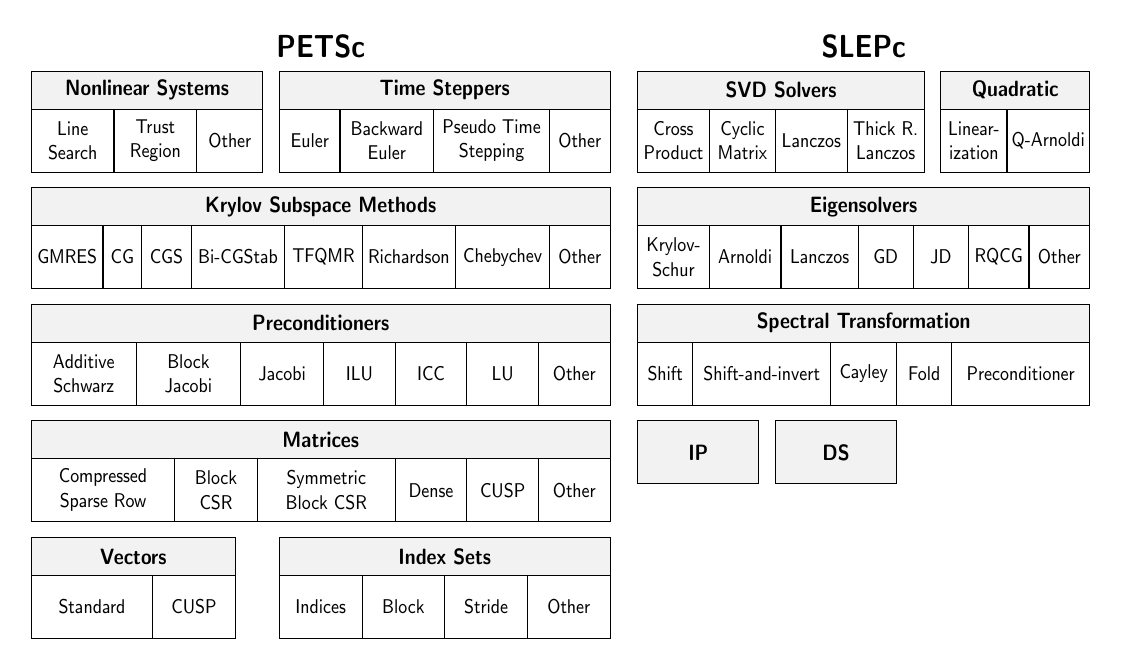
\begin{tikzpicture}[xscale=0.7,yscale=0.8] 
  \tikzstyle{interface}=[fill=black!5,font=\sffamily\bfseries]
  \tikzstyle{implem}=[font=\sffamily\small,text badly centered]
  \tikzstyle{every node}=[transform shape]
  \node[above,text centered,font=\sffamily\bfseries\Large] at (5.25,9.1) {PETSc};
  \draw[interface] (0,1) rectangle node {Vectors} +(3.7,0.6);
  \draw[implem] (0,0) rectangle node {Standard} ++(2.2,1) ++(0,-1)
                      rectangle node {CUSP} ++(1.5,1) ++(0,-1);
  \draw[interface] (4.5,1) rectangle node {Index Sets} +(6,0.6);
  \draw[implem] (4.5,0) rectangle node {Indices} ++(1.5,1) ++(0,-1) 
                rectangle node {Block} ++(1.5,1) ++(0,-1)
                rectangle node {Stride} ++(1.5,1) ++(0,-1)
                rectangle node {Other} ++(1.5,1);
  \draw[interface] (0,2.85) rectangle node {Matrices} +(10.5,0.6);
  \draw[implem] (0,1.85) rectangle node[text width=2.5cm] {Compressed Sparse Row} ++(2.6,1) ++(0,-1) 
                rectangle node[text width=1.3cm] {Block CSR} ++(1.5,1) ++(0,-1) 
                rectangle node[text width=2.3cm] {Symmetric Block CSR} ++(2.5,1) ++(0,-1) 
                rectangle node {Dense} ++(1.3,1) ++(0,-1) 
                rectangle node {CUSP} ++(1.3,1) ++(0,-1) 
                rectangle node {Other} ++(1.3,1);
  \draw[interface] (0,4.7) rectangle node {Preconditioners} +(10.5,0.6);
  \draw[implem] (0,3.7) rectangle node[text width=1.7cm] {Additive Schwarz} ++(1.9,1) ++(0,-1) 
                rectangle node[text width=1.7cm] {Block Jacobi} ++(1.9,1) ++(0,-1) 
                rectangle node {Jacobi} ++(1.5,1) ++(0,-1) 
                rectangle node {ILU} ++(1.3,1) ++(0,-1) 
                rectangle node {ICC} ++(1.3,1) ++(0,-1) 
                rectangle node {LU} ++(1.3,1) ++(0,-1) 
                rectangle node {Other} ++(1.3,1);
  \draw[interface] (0,6.55) rectangle node {Krylov Subspace Methods} +(10.5,0.6);
  \draw[implem] (0,5.55) rectangle node {GMRES} ++(1.3,1) ++(0,-1) 
                rectangle node {CG} ++(0.7,1) ++(0,-1) 
                rectangle node {CGS} ++(0.9,1) ++(0,-1) 
                rectangle node {Bi-CGStab} ++(1.7,1) ++(0,-1) 
                rectangle node {TFQMR} ++(1.4,1) ++(0,-1) 
                rectangle node {Richardson} ++(1.7,1) ++(0,-1) 
                rectangle node {Chebychev} ++(1.7,1) ++(0,-1) 
                rectangle node {Other} ++(1.1,1);
  \draw[interface] (0,8.4) rectangle node {Nonlinear Systems} +(4.2,0.6);
  \draw[implem] (0,7.4) rectangle node[text width=1.2cm] {Line Search} ++(1.5,1) ++(0,-1) 
                rectangle node[text width=1.2cm] {Trust Region} ++(1.5,1) ++(0,-1) 
                rectangle node {Other} ++(1.2,1);
  \draw[interface] (4.5,8.4) rectangle node {Time Steppers} +(6,0.6);
  \draw[implem] (4.5,7.4) rectangle node {Euler} ++(1.1,1) ++(0,-1) 
                rectangle node[text width=1.5cm] {Backward Euler} ++(1.7,1) ++(0,-1) 
                rectangle node[text width=1.8cm] {Pseudo Time Stepping} ++(2.1,1) ++(0,-1) 
                rectangle node {Other} ++(1.1,1);
  \node[above,text centered,font=\sffamily\bfseries\Large] at (15.1,9.1) {SLEPc};
  \draw[interface] (11,8.4) rectangle node {SVD Solvers} +(5.2,0.6);
  \draw[implem] (11,7.4) rectangle node[text width=1.2cm] {Cross Product} ++(1.3,1) ++(0,-1) 
                rectangle node[text width=1.2cm] {Cyclic Matrix} ++(1.2,1) ++(0,-1) 
                rectangle node {Lanczos} ++(1.3,1) ++(0,-1) 
                rectangle node[text width=1.7cm] {Thick R. Lanczos} ++(1.4,1);
  \draw[interface] (16.5,8.4) rectangle node {Quadratic} +(2.7,0.6);
  \draw[implem] (16.5,7.4) rectangle node[text width=1.2cm] {Linear\-ization} ++(1.2,1) ++(0,-1) 
                rectangle node[text width=1.7cm] {Q-Arnoldi} ++(1.5,1);
  \draw[interface] (11,6.55) rectangle node {Eigensolvers} +(8.2,0.6);
  \draw[implem] (11,5.55) rectangle node[text width=1.2cm] {Krylov-Schur} ++(1.3,1) ++(0,-1) 
                rectangle node {Arnoldi} ++(1.3,1) ++(0,-1) 
                rectangle node {Lanczos} ++(1.4,1) ++(0,-1) 
                rectangle node {GD} ++(1.0,1) ++(0,-1)
                rectangle node {JD} ++(1.0,1) ++(0,-1)
                rectangle node {RQCG} ++(1.1,1) ++(0,-1)
                rectangle node {Other} ++(1.1,1);
  \draw[interface] (11,4.7) rectangle node {Spectral Transformation} +(8.2,0.6);
  \draw[implem] (11,3.7) rectangle node {Shift} ++(1,1) ++(0,-1) 
                rectangle node {Shift-and-invert} ++(2.5,1) ++(0,-1) 
                rectangle node {Cayley} ++(1.2,1) ++(0,-1) 
                rectangle node {Fold} ++(1,1) ++(0,-1)
                rectangle node {Preconditioner} ++(2.5,1);
  \draw[interface] (11,2.45) rectangle node {IP} +(2.2,1.0);
  \draw[interface] (13.5,2.45) rectangle node {DS} +(2.2,1.0);
\end{tikzpicture}
\caption{\label{fig:slepc}Numerical components of \petsc and \slepc.}
\end{figure}

	Each of these components consists of an abstract interface (simply a set of calling sequences) and one or more implementations using particular data structures. Both \petsc and \slepc are written in C, which lacks direct support for object-oriented programming. However, it is still possible to take advantage of the three basic principles of object-oriented programming to manage the complexity of such a large package. \petsc uses data \emph{encapsulation} in both vector and matrix data objects. Application code accesses data through function calls. Also, all the operations are supported through \emph{polymorphism}. The user calls a generic interface routine, which then selects the underlying routine that handles the particular data structure. Finally, \petsc also uses \emph{inheritance} in its design. All the objects are derived from an abstract base object. From this fundamental object, an abstract base object is defined for each \petsc\ object (\texttt{Mat}, \texttt{Vec} and so on), which in turn has a variety of instantiations that, for example, implement different matrix storage formats.

	\petsc/\slepc provide clean and effective codes for the various phases of solving PDEs, with a uniform approach for each class of problems.  This design enables easy comparison and use of different algorithms (for example, to experiment with different Krylov subspace methods, preconditioners, or eigensolvers). Hence, \petsc, together with \slepc, provide a rich environment for modeling scientific applications as well as for rapid algorithm design and prototyping.

	Options can be specified by means of calls to subroutines in the source code and also as command-line arguments. Runtime options allow the user to test different tolerances, for example, without having to recompile the program. Also, since \petsc provides a uniform interface to all of its linear solvers ---the Conjugate Gradient, GMRES, etc.--- and a large family of preconditioners ---block Jacobi, overlapping additive Schwarz, etc.---, one can compare several combinations of method and preconditioner by simply specifying them at execution time. \slepc shares this good property.
	
	The components enable easy customization and extension of both algorithms and implementations. This approach promotes code reuse and flexibility, and separates the issues of parallelism from the choice of algorithms.  The \petsc infrastructure creates a foundation for building large-scale applications.

%---------------------------------------------------
\section{Installation}
\label{sec:inst}

	This section describes \slepc's installation procedure.  
	Previously to the installation of \slepc, the system must have an appropriate version of \petsc\ installed. Table \ref{tab:ver} shows a list of \slepc versions and their corresponding \petsc\ versions. \slepc versions marked as major releases are those which incorporate some new functionality. The rest are just adaptations required for a new \petsc\ release and may also include bug fixes.

\begin{table}
\centering
\begin{tabular}{ccccc}
\slepc version &     \petsc versions &  Major  & Release date \\ \hline
         2.1.0 &               2.1.0 & $\star$ & Not released \\
         2.1.1 & 2.1.1, 2.1.2, 2.1.3 &         & Dec 2002     \\ 
         2.1.5 &        2.1.5, 2.1.6 &         & May 2003     \\ 
         2.2.0 &               2.2.0 & $\star$ & Apr 2004     \\
         2.2.1 &               2.2.1 & $\star$ & Aug 2004     \\
         2.3.0 &               2.3.0 & $\star$ & Jun 2005     \\
         2.3.1 &               2.3.1 &         & Mar 2006     \\
         2.3.2 &        2.3.1, 2.3.2 & $\star$ & Oct 2006     \\
         2.3.3 &               2.3.3 & $\star$ & Jun 2007     \\ 
         3.0.0 &               3.0.0 & $\star$ & Feb 2009     \\
         3.1   &               3.1   & $\star$ & Aug 2010     \\
         3.2   &               3.2   & $\star$ & Oct 2011     \\
         3.3   &               3.3   & $\star$ & Aug 2012     \\ \hline
\end{tabular}
\caption{\label{tab:ver} Correspondence between \slepc and \petsc\ releases.}
\end{table}

	The installation process for \slepc is very similar to \petsc, with two stages: configuration and compilation. \slepc's configuration is much simpler because most of the configuration information is taken from \petsc, including compiler options and scalar type (real or complex). See \S\ref{sec:opt-inst} for a discussion of options that are most relevant for \slepc. Several configurations can coexist in the same directory tree, so that for instance one can have \slepc libraries compiled with real scalars as well as with complex scalars. This is explained in \S\ref{sec:mult-inst}. Also, system-based installation is also possible with the \Verb!--prefix! option, as discussed in \S\ref{sec:prefix-inst}.

\subsection{Standard Installation}
\label{sec:std-inst}

	The basic steps for the installation are described next. Note that prior to these steps, optional packages must have been installed. If any of these packages is installed afterwards, reconfiguration and recompilation is necessary. Refer to \S\ref{sec:opt-inst} and \S\ref{sec:wrap} for details about installation of some of these packages.

\begin{enumerate}
	\item Unbundle the distribution file with 
	\begin{Verbatim}[fontsize=\small]
	$ tar xzf slepc-3.3-p0.tar.gz
	\end{Verbatim}
        or an equivalent command. This will create a directory and unpack the software there.
	\item Set the environment variable \ident{SLEPC\_DIR} to the full path of the \slepc home directory. For example, under the \texttt{bash} shell:
	\begin{Verbatim}[fontsize=\small]
	$ export SLEPC_DIR=/home/username/slepc-3.3
	\end{Verbatim}
	In addition to this variable, \ident{PETSC\_DIR} and \ident{PETSC\_ARCH} must also be set appropriately (see \S\ref{sec:prefix-inst} for a case in which \ident{PETSC\_ARCH} is not required), for example
	\begin{Verbatim}[fontsize=\small]
	$ export PETSC_DIR=/home/username/petsc-3.3
	$ export PETSC_ARCH=arch-darwin-c-debug
	\end{Verbatim}
	\item\label{step-config} Change to the \slepc directory and run the configuration script:
	\begin{Verbatim}[fontsize=\small]
	$ cd $SLEPC_DIR
	$ ./configure
	\end{Verbatim}
	\item If the configuration was successful, build the libraries:
	\begin{Verbatim}[fontsize=\small]
	$ make
	\end{Verbatim}
	\item After the compilation, try running some test examples with
	\begin{Verbatim}[fontsize=\small]
	$ make test
	\end{Verbatim}
        Examine the output for any obvious errors or problems.
\end{enumerate}
	
\subsection{Configuration Options}
\label{sec:opt-inst}

Several options are available in \slepc's configuration script. To see all available options, type \Verb!./configure --help!.

In \slepc, configure options have the following purposes:
\begin{itemize}
%\item Build \slepc with Python interfaces, as explained in \S\ref{sec:py-inst}.
\item Specify a directory for prefix-based installation, as explained in \S\ref{sec:prefix-inst}.
\item Enable external eigensolver packages. For example, to use \arpack, specify the following options (with the appropriate paths):
	\begin{Verbatim}[fontsize=\small]
	$ ./configure --with-arpack-dir=/usr/software/ARPACK 
	              --with-arpack-flags=-lparpack,-larpack
	\end{Verbatim}
Section \ref{sec:wrap} provides more details related to use of external libraries.
\end{itemize}

Additionally, \petsc's configuration script provides a very long list of options that are relevant to \slepc. Here is a list of options that may be useful. Note that these are options of \petsc that apply to both \petsc and \slepc, in such a way that it is not possible to, e.g., build \petsc without debugging and \slepc with debugging.
\begin{itemize}
\item Add \Verb!--with-scalar-type=complex! to build complex scalar versions of all libraries. See below a note related to complex scalars.
\item Build single precision versions with \Verb!--with-precision=single!. In most applications, this can achieve a significant reduction of memory requirements, and a moderate reduction of computing time. Also, quadruple precision (128-bit floating-point representation) is also available on systems using the \texttt{gcc-4.6} compiler, using \Verb!--with-precision=__float128!.
\item Enable use from Fortran. By default, \petsc's configure looks for an appropriate Fortran compiler. If not required, this can be disabled with \Verb!--without-fortran!. If required but not correctly detected, the compiler to be used can be specified with a configure option. In the case of Fortran 90, additional options are available for building interfaces and datatypes.
\item If not detected, use \Verb!--with-blas-lapack-lib! to specify the location of \blas and \lapack. If \slepc's configure complains about some missing \lapack subroutines, reconfigure \petsc with option \Verb!--download-f2cblaslapack!.
\item Enable external libraries that provide direct linear solvers or preconditioners, such as MUMPS, hypre, or SuperLU; for example, \Verb!--download-mumps!. These are especially relevant for \slepc in the case that a spectral transformation is used, see chapter \ref{cap:st}.
\item Enable use from C++, \Verb!--with-clanguage=C++!.
\item Add \Verb!--with-64-bit-indices=1! to use 4 byte integers (\texttt{long long}) for indexing in vectors and matrices. This is only needed when working with over roughly 2 billion unknowns.
\item Build shared libraries, \Verb!--with-shared-libraries=1!, for smaller executables whose symbols are resolved at run time.
\item Error-checking code can be disabled with \Verb!--with-debugging=no!, but this is only recommended in production runs of well-tested applications.
\item Enable GPU computing setting \Verb!--with-cuda=1! and other options, see \S\ref{sec:gpu} for details.
\end{itemize}

\medskip
\textbf{Note about complex scalar versions}: \petsc supports the use of complex scalars by defining the data type \ident{PetscScalar} either as a real or complex number. This implies that two different versions of the \petsc libraries can be built separately, one for real numbers and one for complex numbers, but they cannot be used at the same time. \slepc inherits this property. In \slepc it is not possible to completely separate real numbers and complex numbers because the solution of non-symmetric real-valued eigenvalue problems may be complex. \slepc has been designed trying to provide a uniform interface to manage all the possible cases. However, there are slight differences between the interface in each of the two versions. In this manual, differences are clearly identified.

\subsection{Installing Multiple Configurations in a Single Directory Tree}
\label{sec:mult-inst}

Often, it is necessary to build two (or more) versions of the libraries that differ in a few configuration options. For instance, versions for real and complex scalars, or versions for double and single precision, or versions with debugging and optimized. In a standard installation, this is handled by building all versions in the same directory tree, as explained below, so that source code is not replicated unnecessarily. In contrast, in prefix-based installation where source code is not present, the issue of multiple configurations is handled differently, as explained in \S\ref{sec:prefix-inst}.

In a standard installation, the different configurations are identified by a unique name that is assigned to the environment variable \ident{PETSC\_ARCH}. Let us illustrate how to set up \petsc with two configurations. First, set a value of \ident{PETSC\_ARCH} and proceed with the installation of the first one:
	\begin{Verbatim}[fontsize=\small]
	$ cd $PETSC_DIR
	$ export PETSC_ARCH=arch-linux-gnu-c-debug-real
	$ ./configure --with-scalar-type=real
	$ make all test
	\end{Verbatim}
Note that if \ident{PETSC\_ARCH} is not given a value, \petsc suggests one for us. After this, a subdirectory named \texttt{\$PETSC\_ARCH} is created within \texttt{\$PETSC\_DIR}, that stores all information associated to that configuration, including the built libraries, configuration files, automatically generated source files, and log files. For the second configuration, proceed similarly:
	\begin{Verbatim}[fontsize=\small]
	$ cd $PETSC_DIR
	$ export PETSC_ARCH=arch-linux-gnu-c-debug-complex
	$ ./configure --with-scalar-type=complex
	$ make all test
	\end{Verbatim}
The value of \ident{PETSC\_ARCH} in this case must be different than the previous one. It is better to set the value of \ident{PETSC\_ARCH} explicitly, because the name suggested by \texttt{configure} may coincide with an existing value, thus overwriting a previous configuration. After successful installation of the second configuration, two \texttt{\$PETSC\_ARCH} directories exist within \texttt{\$PETSC\_DIR}, and the user can easily choose to build his/her application with either configuration by simply changing the value of \ident{PETSC\_ARCH}.

The configuration of two versions of \slepc in the same directory tree is very similar. The only important restriction is that the value of \ident{PETSC\_ARCH} used in \slepc must exactly match an existing \petsc configuration, that is, a directory \texttt{\$PETSC\_DIR/\$PETSC\_ARCH} must exist.

\subsection{Prefix-based Installation}
\label{sec:prefix-inst}

Both \petsc and \slepc allow for prefix-based installation. This consists in specifying a directory to which the files generated during the building process are to be copied.

In \petsc, if an installation directory has been specified during configuration (with option \Verb!--prefix! in step \ref{step-config} of \S\ref{sec:std-inst}), then after building the libraries the relevant files are copied to that directory by typing
	\begin{Verbatim}[fontsize=\small]
	$ make install
	\end{Verbatim}
	This is useful for building as a regular user and then copying the libraries and include files to the system directories as root.

To be more precise, suppose that the configuration was done with \texttt{-{}-prefix=/opt/petsc-3.3-linux-gnu-c-debug}. Then, \texttt{make install} will create directory \texttt{/opt/petsc-3.3-linux-gnu-c-debug} if it does not exist, and create subdirectories \texttt{lib}, \texttt{conf}, and \texttt{include}, that will store the libraries, the configuration files, and the header files, respectively. Note that the source code files are not copied, nor the documentation, so the size of the installed directory will be much smaller than the original one. For that reason, it is no longer necessary to allow for several configurations to share a directory tree. In other words, in a prefix-based installation, variable \ident{PETSC\_ARCH} loses significance and must be unset. To maintain several configurations, one should specify different prefix directories, typically with a name that informs about the configuration options used.

In order to prepare a prefix-based installation of \slepc that uses a prefix-based installation of \petsc, start by setting the appropriate value of \ident{PETSC\_DIR}. Then, run \slepc's configure with a prefix directory.
	\begin{Verbatim}[fontsize=\small,numbers=none]
	$ export PETSC_DIR=/opt/petsc-3.3-linux-gnu-c-debug
	$ unset PETSC_ARCH
	$ cd $SLEPC_DIR
	$ ./configure --prefix=/opt/slepc-3.3-linux-gnu-c-debug
	$ make PETSC_ARCH=arch-installed-petsc
	$ make PETSC_ARCH=arch-installed-petsc install
	$ export SLEPC_DIR=/opt/slepc-3.3-linux-gnu-c-debug
	\end{Verbatim}
Note that it is important to unset the value of \ident{PETSC\_ARCH} before \slepc's configure. The special value \texttt{arch-installed-petsc} of the \ident{PETSC\_ARCH} variable is required only during \slepc's build, and should not be used afterwards.

%\subsection{Building Python Interfaces}
%\label{sec:py-inst}

%---------------------------------------------------
\section{Running SLEPc Programs}

Before using \slepc, the user must first set the environment variable
\ident{SLEPC\_DIR}, indicating the full path of the directory containing \slepc. For example, under the \texttt{bash} shell, a command of the form
	\begin{Verbatim}[fontsize=\small]
	$ export SLEPC_DIR=/software/slepc-3.3
	\end{Verbatim}
can be placed in the user's \Verb!.bashrc! file.
The \ident{SLEPC\_DIR} directory can be either a standard installation \slepc directory, or a prefix-based installation directory, see \S\ref{sec:prefix-inst}.
In addition, the user must set the environment variables required by \petsc, that is, \ident{PETSC\_DIR}, to indicate the full path of the \petsc directory, and \ident{PETSC\_ARCH} to specify a particular architecture and set of options. Note that \ident{PETSC\_ARCH} should not be set in the case of prefix-based installations.

All \petsc programs use the MPI (Message Passing Interface) standard
for message-passing communication \citep{MPI-Forum:1994:MMI}.  Thus, to execute
\slepc programs, users must know the procedure for launching MPI jobs
on their selected computer system(s).  For instance, when using the
\mpich\ implementation of MPI and many others, the \texttt{mpirun} command can be used to initiate a program as in the following example that uses eight processes:
	\begin{Verbatim}[fontsize=\small]
	$ mpirun -np 8 slepc_program [command-line options]
	\end{Verbatim}
In MPI-2 compliant systems, the command \texttt{mpiexec} can be used instead. Note that MPI may be deactivated during configuration of \petsc, if one wants to run only serial programs in a laptop, for example.

All \petsc-compliant programs support the use of the \Verb!-h!
or \Verb!-help! option as well as the \Verb!-v! or \Verb!-version! option. In the case of \slepc programs, specific information for \slepc is also displayed.

%---------------------------------------------------
\section{Writing SLEPc Programs}

	Most \slepc programs begin with a call to \rutina{SlepcInitialize}
	\begin{Verbatim}[fontsize=\small]
	SlepcInitialize(int *argc,char ***argv,char *file,char *help);
	\end{Verbatim}
which initializes \slepc, \petsc and MPI. This subroutine is very similar to \rutina{PetscInitialize}, and the arguments have the same meaning. In fact, internally \rutina{SlepcInitialize} calls \rutina{PetscInitialize}.

	After this initialization, \slepc programs can use communicators defined by \petsc. In most cases users can employ the communicator \ident{PETSC\_COMM\_WORLD} to indicate all processes in a given run and \ident{PETSC\_COMM\_SELF} to indicate a single process. MPI provides routines for generating new communicators consisting of subsets of processes, though most users rarely need to use these features. \slepc users need not program much message passing directly with MPI, but they must be familiar with the basic concepts of message passing and distributed memory computing.

	All \slepc programs should call \rutina{SlepcFinalize} as their final (or nearly final) statement
	\begin{Verbatim}[fontsize=\small]
	ierr = SlepcFinalize();
	\end{Verbatim}
This routine handles operations to be executed at the conclusion of the program, and calls \rutina{PetscFinalize} if \rutina{SlepcInitialize} began \petsc.

\medskip
\textbf{Note to Fortran Programmers}: In this manual all the examples and calling sequences are given for the C/C++ programming languages. However, Fortran programmers can use most of the functionality of \slepc and \petsc from Fortran, with only minor differences in the user interface. For instance, the two functions mentioned above have their corresponding Fortran equivalent:
	\begin{Verbatim}[fontsize=\small]
	call SlepcInitialize(file,ierr)
	call SlepcFinalize(ierr)
	\end{Verbatim}
Section \ref{sec:fortran} provides a summary of the differences between using \slepc from Fortran and C/C++, as well as a complete Fortran example. 

%---------------------------------------------------
\subsection{Simple SLEPc Example}
\label{sec:simpleex}

	A simple example is listed next that solves an eigenvalue problem associated with the one-dimensional Laplacian operator discretized with finite differences. This example can be found in \Verb!${SLEPC_DIR}/src/eps/examples/tutorials/ex1.c!. Following the code we highlight a few of the most important parts of this example.  

\MyVerbatimInput{ex1.c}

\subsubsection*{Include Files}

The C/C++ include files for \slepc should be used via statements such as
	\begin{Verbatim}[fontsize=\small]
	#include "slepceps.h"
	\end{Verbatim}
where \Verb!slepceps.h! is the include file for the \ident{EPS} component. Each \slepc program must specify an include file that corresponds to the highest level \slepc objects needed within the program; all of the required lower level include files are automatically included within the higher level files. For example, \Verb!slepceps.h! includes \Verb!slepcst.h! (spectral transformations), and \Verb!slepcsys.h! (base \slepc file). Some \petsc header files are included as well, such as \Verb!petscksp.h!. The \slepc include files are located in the directory \Verb!${SLEPC_DIR}/include!.

\subsubsection*{The Options Database}

All the \petsc functionality related to the options database is available in \slepc. This allows the user to input control data at run time very easily. In this example the command \Verb!PetscOptionsGetInt(PETSC_NULL,"-n",&n,PETSC_NULL);! checks whether the user has provided a command line option to set the value of \Verb!n!, the problem dimension.  If so, the variable \Verb!n! is set accordingly; otherwise, \Verb!n! remains unchanged.

\subsubsection*{Vectors and Matrices}

Usage of matrices and vectors in \slepc is exactly the same as in \petsc. The user can create a new parallel or sequential matrix, \texttt{A}, which has \texttt{M} global rows and \texttt{N} global columns, with 
	\begin{Verbatim}[fontsize=\small]
	MatCreate(MPI_Comm comm,Mat *A);
	MatSetSizes(Mat A,PetscInt m,PetscInt n,PetscInt M,PetscInt N);
	MatSetFromOptions(Mat A);
	MatSetUp(Mat A);
	\end{Verbatim}
where the matrix format can be specified at runtime. The example creates a matrix, sets the nonzero values with \rutina{MatSetValues} and then assembles it.

\subsubsection*{Eigensolvers}

Usage of eigensolvers is very similar to other kinds of solvers provided by \petsc. After creating the matrix (or matrices) that define the problem, $Ax = kx$ (or $Ax=kBx$), the user can then use \ident{EPS} to solve the system with the following sequence of commands: 
\findex{EPSCreate} \findex{EPSSetOperators} \findex{EPSSetProblemType}
\findex{EPSSetFromOptions} \findex{EPSSolve} \findex{EPSDestroy}
\findex{EPSGetConverged} \findex{EPSGetEigenpair}
	\begin{Verbatim}[fontsize=\small,numbers=none]
	EPSCreate(MPI_Comm comm,EPS *eps);
	EPSSetOperators(EPS eps,Mat A,Mat B);
        EPSSetProblemType(EPS eps,EPSProblemType type);
	EPSSetFromOptions(EPS eps);
	EPSSolve(EPS eps);
	EPSGetConverged(EPS eps,PetscInt *nconv);
	EPSGetEigenpair(EPS eps,PetscInt i,PetscScalar *kr,PetscScalar *ki,Vec xr,Vec xi);
	EPSDestroy(EPS eps);
	\end{Verbatim} 
The user first creates the \ident{EPS} context and sets the operators associated with the eigensystem as well as the problem type. The user then sets various options for customized solution, solves the problem, retrieves the solution, and finally destroys the \ident{EPS} context. Chapter~\ref{cap:eps} describes in detail the \ident{EPS} package, including
the options database that enables the user to customize the solution process at runtime by selecting the solution algorithm and also specifying the convergence tolerance, the number of eigenvalues, the dimension of the subspace, etc.

\subsubsection*{Spectral Transformation}

In the example program shown above there is no explicit reference to spectral transformations. However, an \ident{ST} object is handled internally so that the user is able to request different transformations such as shift-and-invert. Chapter~\ref{cap:st} describes the \ident{ST} package in detail.

\subsubsection*{Error Checking}

	All \slepc routines return an integer indicating whether an error has occurred during the call. The error code is set to be nonzero if an error has been detected; otherwise, it is zero. The \petsc macro \Verb!CHKERRQ(ierr)! checks the value of \Verb!ierr! and calls the \petsc error handler upon error detection. \Verb!CHKERRQ(ierr)! should be placed after all subroutine calls to enable a complete error traceback. See the \petsc documentation for full details.

\subsection{Writing Application Codes with SLEPc}

Several example programs demonstrate the software usage and can serve as templates for developing custom applications. They are scattered throughout the SLEPc directory tree, in particular in the \Verb!examples/tutorials! directories under each class subdirectory.

To write a new application program using \slepc, we suggest the following procedure:
\begin{enumerate}
\item Install and test \slepc according to the instructions given in the documentation.
\item Copy the \slepc example that corresponds to the class of problem of interest (e.g., singular value decomposition).
\item Copy the makefile within the example directory (or create a new one as explained below); compile and run the example program.
\item Use the example program as a starting point for developing a custom code.
\end{enumerate}

	Application program makefiles can be set up very easily just by including one file from the \slepc makefile system. All the necessary \petsc{} definitions are loaded automatically. The following sample makefile illustrates how to build C and Fortran programs:

	\begin{Verbatim}[fontsize=\small]
default: ex1

include ${SLEPC_DIR}/conf/slepc_common

ex1: ex1.o chkopts
	-${CLINKER} -o ex1 ex1.o ${SLEPC_LIB}
	${RM} ex1.o

ex1f: ex1f.o chkopts
	-${FLINKER} -o ex1f ex1f.o ${SLEPC_LIB}
	${RM} ex1f.o
	\end{Verbatim}



%-------------------------------------------------------
% SLEPc Users Manual
%-------------------------------------------------------
\chapter{\label{cap:eps}EPS: Eigenvalue Problem Solver}
%-------------------------------------------------------

\noindent The Eigenvalue Problem Solver (\ident{EPS}) is the main object provided by \slepc. It is used to specify an eigenvalue problem, either in standard or generalized form, and provides uniform and efficient access to all of the eigensolvers included in the package. Conceptually, the level of abstraction occupied by \ident{EPS} is similar to other solvers in \petsc\ such as \ident{KSP} for solving linear systems of equations.
	
\section{\label{sec:eig}Eigenvalue Problems}

	In this section, we present very briefly some basic concepts about eigenvalue problems as well as general techniques used to solve them. The description is not intended to be exhaustive. The objective is simply to define terms that will be referred to throughout the rest of the manual. Readers who are familiar with the terminology and the solution approach can skip this section. For a more comprehensive description, we refer the reader to monographs such as \citep{Stewart:2001:MAV}, \citep{Bai:2000:TSA}, \citep{Saad:1992:NML} or \citep{Parlett:1980:SEP}. A historical perspective of the topic can be found in \citep{Golub:2000:EC2}. See also the \slepc \hyperlink{str}{technical reports}.

In the standard formulation, the eigenvalue problem consists in the determination of $\lambda\in\mathbb{C}$ for which the equation
\begin{equation}
Ax=\lambda x\;\;\label{eq:eigstd}
\end{equation}
has nontrivial solution, where $A\in\mathbb{C}^{n\times n}$ and $x\in\mathbb{C}^n$. The scalar $\lambda$ and the vector $x$ are called eigenvalue and (right) eigenvector, respectively. Note that they can be complex even when the matrix is real. If $\lambda$ is an eigenvalue of $A$ then $\bar{\lambda}$ is an eigenvalue of its conjugate transpose, $A^*$, or equivalently
\begin{equation}
y^*\!A=\lambda\, y^*\;\;,\label{eq:eigstdleft}
\end{equation}
where $y$ is called the left eigenvector.

	In many applications, the problem is formulated as 
\begin{equation}
Ax=\lambda Bx\;\;,\label{eq:eiggen}
\end{equation}
where $B\in\mathbb{C}^{n\times n}$, which is known as the generalized eigenvalue problem. Usually, this problem is solved by reformulating it in standard form, for example $B^{-1}Ax=\lambda x$ if $B$ is non-singular.

	\slepc focuses on the solution of problems in which the matrices are large and sparse. Hence, only methods that preserve sparsity are considered.
	These methods obtain the solution from the information generated by the application of the operator to various vectors (the operator is a simple function of matrices $A$ and $B$), that is, matrices are only used in matrix-vector products. This not only maintains sparsity but allows the solution of problems in which matrices are not available explicitly.

In practical analyses, from the $n$ possible solutions, typically only a few eigenpairs $(\lambda,x)$ are considered relevant, either in the extremities of the spectrum, in an interval, or in a region of the complex plane.
Depending on the application, either eigenvalues or eigenvectors or both are required. In some cases, left eigenvectors are also of interest.
	
\paragraph{Projection Methods.}

	Most eigensolvers provided by \slepc perform a Rayleigh-Ritz projection for extracting the spectral approximations, that is, they project the problem onto a low-dimensional subspace that is built appropriately. Suppose that an orthogonal basis of this subspace is given by $V_j=[v_1,v_2,\ldots,v_j]$. If the solutions of the projected (reduced) problem $B_js=\theta s$ (i.e., $V_j^TAV_j=B_j$) are assumed to be $(\theta_i,s_i)$, $i=1,2,\ldots,j$, then the approximate eigenpairs $(\tilde{\lambda}_i,\tilde{x}_i)$ of the original problem (Ritz value and Ritz vector) are obtained as
\begin{eqnarray}
\tilde{\lambda}_i=\theta_i\quad,\\
\quad\tilde{x}_i=V_js_i\quad.
\end{eqnarray}
Starting from this general idea, eigensolvers differ from each other in which subspace is used, how it is built and other technicalities aimed at improving convergence, reducing storage requirements, etc.

	The subspace
\begin{equation}
\mathcal{K}_m(A,v)\equiv\mathrm{span}\left\{v,Av,A^2v,\ldots,A^{m-1}v\right\}\;\;,\label{eq:krylov}
\end{equation}
is called the $m$-th Krylov subspace corresponding to $A$ and $v$. Methods that use subspaces of this kind to carry out the projection are called Krylov methods. One example of such methods is the Arnoldi algorithm: starting with $v_1$, $\|v_1\|_2=1$, the Arnoldi basis generation process can be expressed by the recurrence
\begin{equation}
v_{j+1}h_{j+1,j}=w_j=Av_j-\sum_{i=1}^jh_{i,j}v_i\quad,
\end{equation}
where $h_{i,j}$ are the scalar coefficients obtained in the Gram-Schmidt orthogonalization of $Av_j$ with respect to $v_i$, $i=1,2,\ldots,j$, and $h_{j+1,j}=\|w_j\|_2$. Then, the columns of $V_j$ span the Krylov subspace $\mathcal{K}_j(A,v_1)$ and $Ax=\lambda x$ is projected into $H_js=\theta s$, where $H_j$ is an upper Hessenberg matrix with elements $h_{i,j}$, which are 0 for $i\geq j+2$. The related Lanczos algorithms obtain a projected matrix that is tridiagonal.

	A generalization to the above methods are the block Krylov strategies, in which the starting vector $v_1$ is replaced by a full rank $n\times p$ matrix $V_1$, which allows for better convergence properties when there are multiple eigenvalues and can provide better data management on some computer architectures. Block tridiagonal and block Hessenberg matrices are then obtained as projections.

	It is generally assumed (and observed) that the Lanczos and Arnoldi algorithms find solutions at the extremities of the spectrum. Their convergence pattern, however, is strongly related to the eigenvalue distribution. Slow convergence may be experienced in the presence of tightly clustered eigenvalues. The maximum allowable $j$ may be reached without having achieved convergence for all desired solutions. Then, restarting is usually a useful technique and different strategies exist for that purpose. However, convergence can still be very slow and acceleration strategies must be applied. Usually, these techniques consist in computing eigenpairs of a transformed operator and then recovering the solution of the original problem. The aim of these transformations is twofold. On one hand, they make it possible to obtain eigenvalues other than those lying in the boundary of the spectrum. On the other hand, the separation of the eigenvalues of interest is improved in the transformed spectrum thus leading to faster convergence. The most commonly used spectral transformation is called shift-and-invert, which works with operator $(A-\sigma I)^{-1}$. It allows the computation of eigenvalues closest to $\sigma$ with very good separation properties. When using this approach, a linear system of equations, $(A-\sigma I)y=x$, must be solved in each iteration of the eigenvalue process.

\paragraph{Preconditioned Eigensolvers.}
	In many applications, Krylov eigensolvers perform very well because Krylov subspaces are optimal in a certain theoretical sense. However, these methods may not be appropriate in some situations such as the computation of interior eigenvalues. The spectral transformation mentioned above may not be a viable solution or it may be too costly. For these reasons, other types of eigensolvers such as Davidson and Jacobi-Davidson rely on a different way of expanding the subspace. Instead of satisfying the Krylov relation, these methods compute the new basis vector by the so-called correction equation. The resulting subspace may be richer in the direction of the desired eigenvectors. These solvers may be competitive especially for computing interior eigenvalues. From a practical point of view, the correction equation may be seen as a cheap replacement for the shift-and-invert system of equations, $(A-\sigma I)y=x$. By cheap we mean that it may be solved inaccurately without compromising robustness, via a preconditioned iterative linear solver. For this reason, these are known as \emph{preconditioned} eigensolvers.

\paragraph{Related Problems.}

	In many applications such as the analysis of damped vibrating systems the problem to be solved is a \emph{quadratic eigenvalue problem} (QEP). Another linear algebra problem that is very closely related to the eigenvalue problem is the {\em singular value decomposition\/} (SVD). \slepc provides specific packages for both problems. The reader is referred to chapters \ref{cap:svd} and \ref{cap:qep}.

%---------------------------------------------------
\section{Basic Usage}

	The \ident{EPS} module in \slepc is used in a similar way as \petsc modules such as \ident{KSP}. All the information related to an eigenvalue problem is handled via a context variable. The usual object management functions are available (\ident{EPSCreate}, \ident{EPSDestroy}, \ident{EPSView}, \ident{EPSSetFromOptions}). In addition, the \ident{EPS} object provides functions for setting several parameters such as the number of eigenvalues to compute, the dimension of the subspace, the portion of the spectrum of interest, the requested tolerance or the maximum number of iterations allowed.

	The solution of the problem is obtained in several steps. First of all, the matrices associated to the eigenproblem are specified via \ident{EPSSetOperators} and \ident{EPSSetProblemType} is used to specify the type of problem. Then, a call to \ident{EPSSolve} is done that invokes the subroutine for the selected eigensolver. \ident{EPSGetConverged} can be used afterwards to determine how many of the requested eigenpairs have converged to working accuracy. \ident{EPSGetEigenpair} is finally used to retrieve the eigenvalues and eigenvectors.

	In order to illustrate the basic functionality of the \ident{EPS} package, a simple example is shown in Figure \ref{fig:ex-eps}. The example code implements the solution of a simple standard eigenvalue problem. Code for setting up the matrix $A$ is not shown and error-checking code is omitted.

\begin{figure}
\begin{Verbatim}[fontsize=\small,numbers=left,numbersep=6pt,xleftmargin=15mm]
EPS         eps;       /*  eigensolver context  */
Mat         A;         /*  matrix of Ax=kx      */
Vec         xr, xi;    /*  eigenvector, x       */
PetscScalar kr, ki;    /*  eigenvalue, k        */
PetscInt    j, nconv;
PetscReal   error;

EPSCreate( PETSC_COMM_WORLD, &eps );
EPSSetOperators( eps, A, PETSC_NULL );
EPSSetProblemType( eps, EPS_NHEP );
EPSSetFromOptions( eps );
EPSSolve( eps );
EPSGetConverged( eps, &nconv );
for (j=0; j<nconv; j++) {
  EPSGetEigenpair( eps, j, &kr, &ki, xr, xi );
  EPSComputeRelativeError( eps, j, &error );
}
EPSDestroy( eps );
\end{Verbatim}
\caption{\label{fig:ex-eps}Example code for basic solution with \ident{EPS}.}
\end{figure}

	All the operations of the program are done over a single \ident{EPS} object. This solver context is created in line 8 with the command 
	\findex{EPSCreate}
	\begin{Verbatim}[fontsize=\small]
	EPSCreate(MPI_Comm comm,EPS *eps);
	\end{Verbatim}
	Here \texttt{comm} is the MPI communicator, and \texttt{eps} is the newly formed solver context. The communicator indicates which processes are involved in the \ident{EPS} object. Most of the \ident{EPS} operations are collective, meaning that all the processes collaborate to perform the operation in parallel. 

	Before actually solving an eigenvalue problem with \ident{EPS}, the user must specify the matrices associated to the problem, as in line 9, with the following routine
	\findex{EPSSetOperators}
	\begin{Verbatim}[fontsize=\small]
	EPSSetOperators(EPS eps,Mat A,Mat B);
	\end{Verbatim}
	The example specifies a standard eigenproblem. In the case of a generalized problem, it would be necessary also to provide matrix $B$ as the third argument to the call. The matrices specified in this call can be in any \petsc format. In particular, \ident{EPS} allows the user to solve matrix-free problems by specifying matrices created via \ident{MatCreateShell}. A more detailed discussion of this issue is given in \S\ref{sec:supported}.

	After setting the problem matrices, the problem type is set with \ident{EPSSetProblemType}. This is not strictly necessary since if this step is skipped then the problem type is assumed to be non-symmetric. More details are given in \S\ref{sec:defprob}.
	At this point, the value of the different options could optionally be set by means of a function call such as \ident{EPSSetTolerances} (explained later in this chapter). After this, a call to \ident{EPSSetFromOptions} should be made as in line 11, 
	\findex{EPSSetFromOptions}
	\begin{Verbatim}[fontsize=\small]
	EPSSetFromOptions(EPS eps);
	\end{Verbatim}
	The effect of this call is that options specified at runtime in the command line are passed to the \ident{EPS} object appropriately. In this way, the user can easily experiment with different combinations of options without having to recompile. All the available options as well as the associated function calls are described later in this chapter.

	Line 12 launches the solution algorithm, simply with the command
	\findex{EPSSolve}
	\begin{Verbatim}[fontsize=\small]
	EPSSolve(EPS eps);
	\end{Verbatim}
	The subroutine that is actually invoked depends on which solver has been selected by the user. 
        
        After the call to \ident{EPSSolve} has finished, all the data associated to the solution of the eigenproblem is kept internally. This information can be retrieved with different function calls, as in lines 13 to 17. This part is described in detail in \S\ref{sec:retrsol}.

	Once the \ident{EPS} context is no longer needed, it should be destroyed with the command
	\findex{EPSDestroy}
	\begin{Verbatim}[fontsize=\small]
	EPSDestroy(EPS eps);
	\end{Verbatim}

	The above procedure is sufficient for general use of the \ident{EPS} package. As in the case of the \ident{KSP} solver, the user can optionally explicitly call 
	\findex{EPSSetUp}
	\begin{Verbatim}[fontsize=\small]
	EPSSetUp(EPS eps);
	\end{Verbatim}
before calling \ident{EPSSolve} to perform any setup required for the eigensolver.

	Internally, the \ident{EPS} object works with an \ident{ST} object (spectral transformation, described in chapter \ref{cap:st}). To allow application programmers to set any of the spectral transformation options directly within the code, the following routine is provided to extract the \ident{ST} context,
	\findex{EPSGetST}
	\begin{Verbatim}[fontsize=\small]
	EPSGetST(EPS eps,ST *st);
	\end{Verbatim}
	
	With the command
	\findex{EPSView}
	\begin{Verbatim}[fontsize=\small]
	EPSView(EPS eps,PetscViewer viewer);
	\end{Verbatim}
it is possible to examine the actual values of the different settings of the \ident{EPS} object, including also those related to the associated \ident{ST} object. This is useful for making sure that the solver is using the settings that the user wants.

%---------------------------------------------------
\section{Defining the Problem}
\label{sec:defprob}

	\slepc is able to cope with different kinds of problems. Currently supported problem types are listed in Table \ref{tab:ptype}. An eigenproblem is generalized ($Ax=\lambda Bx$) if the user has specified two matrices (see \ident{EPSSetOperators} above), otherwise it is standard ($Ax=\lambda x$). A standard eigenproblem is Hermitian if matrix $A$ is Hermitian (i.e., $A=A^*$) or, equivalently in the case of real matrices, if matrix $A$ is symmetric (i.e., $A=A^T$). A generalized eigenproblem is Hermitian if matrix $A$ is Hermitian (symmetric) and $B$ is Hermitian (symmetric) and positive (semi-)definite.
A special case of generalized non-Hermitian problem is when $A$ is non-Hermitian but $B$ is Hermitian and positive (semi-)definite, see \S\ref{sec:symm} and \S\ref{sec:purif} for discussion.

\begin{table}[t]
\centering
{\small \begin{tabular}{lll}
Problem Type              & \ident{EPSProblemType}    & Command line key\\\hline
Hermitian                 & \texttt{EPS\_HEP}         & \texttt{-eps\_hermitian}\\
Non-Hermitian             & \texttt{EPS\_NHEP}        & \texttt{-eps\_non\_hermitian}\\
Generalized Hermitian     & \texttt{EPS\_GHEP}        & \texttt{-eps\_gen\_hermitian}\\
Generalized Non-Hermitian & \texttt{EPS\_GNHEP}       & \texttt{-eps\_gen\_non\_hermitian}\\
GNHEP with positive (semi-)definite $B$ & \texttt{EPS\_PGNHEP} & \texttt{-eps\_pos\_gen\_non\_hermitian}\\\hline
\end{tabular} }
\caption{\label{tab:ptype}Problem types considered in \ident{EPS}.}
\end{table}

The problem type can be specified at run time with the corresponding command line key or, more usually, within the program with the function
	\findex{EPSSetProblemType}
	\begin{Verbatim}[fontsize=\small]
	EPSSetProblemType(EPS eps,EPSProblemType type);
	\end{Verbatim}

By default, \slepc assumes that the problem is non-Hermitian. Some eigensolvers are able to exploit symmetry, that is, they compute a solution for Hermitian problems with less storage and/or computational cost than other methods that ignore this property. Also, symmetric solvers may be more accurate. On the other hand, some eigensolvers in \slepc only have a symmetric version and will abort if the problem is non-Hermitian. 
In the case of generalized eigenproblems some considerations apply regarding symmetry, especially in the case of singular $B$. This topic is tackled in \S\ref{sec:symm} and \S\ref{sec:purif}.
For all these reasons, the user is strongly recommended to always specify the problem type in the source code. 

	The type of the problem can be determined with the functions
	\findex{EPSIsGeneralized} \findex{EPSIsHermitian}
	\begin{Verbatim}[fontsize=\small]
	EPSIsGeneralized(EPS eps,PetscTruth *gen);
	EPSIsHermitian(EPS eps,PetscTruth *her);
	\end{Verbatim}

	The user can specify how many eigenvalues (and eigenvectors) to compute. The default is to compute only one. The function
	\findex{EPSSetDimensions}
	\begin{Verbatim}[fontsize=\small]
	EPSSetDimensions(EPS eps,PetscInt nev,PetscInt ncv,PetscInt mpd);
	\end{Verbatim}
allows the specification of the number of eigenvalues to compute, \texttt{nev}. The second argument can be set to prescribe the number of column vectors to be used by the solution algorithm, \texttt{ncv}, that is, the largest dimension of the working subspace. The third argument has to do with a more advanced usage, as explained in \S\ref{sec:large-nev}. These parameters can also be set at run time with the options \Verb!-eps_nev!, \Verb!-eps_ncv! and \Verb!-eps_mpd!. For example, the command line
\begin{Verbatim}[fontsize=\small]
	$ ./program -eps_nev 10 -eps_ncv 24
\end{Verbatim}
requests 10 eigenvalues and instructs to use 24 column vectors. Note that \texttt{ncv} must be at least equal to \texttt{nev}, although in general it is recommended (depending on the method) to work with a larger subspace, for instance $\mathtt{ncv}\geq2\cdot\mathtt{nev}$ or even more. The case that the user requests a relatively large number of eigenpairs is discussed in \S\ref{sec:large-nev}.

	By default, only right eigenvectors are computed. To compute also left eigenvectors, the user should call the next function. Note that support for left eigenvectors is limited and will be extended in future versions of SLEPc.
	\findex{EPSSetLeftVectorsWanted}
	\begin{Verbatim}[fontsize=\small]
	EPSSetLeftVectorsWanted(EPS eps,PetscTruth leftvecs);
	\end{Verbatim}

\paragraph{Eigenvalues of Interest.}

	For the selection of the portion of the spectrum of interest, there are several alternatives. In real symmetric problems, one may want to compute the largest or smallest eigenvalues in magnitude, or the leftmost or rightmost ones, or even all eigenvalues in a given interval. In other problems, in which the eigenvalues can be complex, then one can select eigenvalues depending on the magnitude, or the real part or even the imaginary part. Sometimes the eigenvalues of interest are those closest to a given target value, $\tau$, measuring the distance either in the ordinary way or along the real (or imaginary) axis. Table \ref{tab:portion} summarizes all the possibilities available for the function
	\findex{EPSSetWhichEigenpairs}
	\begin{Verbatim}[fontsize=\small]
	EPSSetWhichEigenpairs(EPS eps,EPSWhich which);
	\end{Verbatim}
which can also be specified at the command line. This criterion is used both for configuring how the eigensolver seeks eigenvalues (note that not all these possibilities are available for all the solvers) and also for sorting the computed values. The default is to compute the largest magnitude eigenvalues, except for those solvers in which this option is not available. There is another exception related to the use of some spectral transformations, see chapter \ref{cap:st}.

	For the sorting criteria relative to a target value, the following function must be called in order to specify such value $\tau$:
	\findex{EPSSetTarget}
	\begin{Verbatim}[fontsize=\small]
	EPSSetTarget(EPS eps,PetscScalar target);
	\end{Verbatim}
or, alternatively, with the command-line key \Verb!-eps_target!. Note that, since the target is defined as a \texttt{PetscScalar}, complex values of $\tau$ are allowed only in the case of complex scalar builds of the SLEPc library.

The use of a target value makes sense if the eigenvalues of interest are located in the interior of the spectrum. Since these eigenvalues are usually more difficult to compute, the eigensolver by itself may not be able to obtain them, and additional tools are normally required. 
There are two possibilities for this:
\begin{itemize}
\item To use harmonic extraction (see \S\ref{sec:harmonic}), a variant of some solvers that allows a better approximation of interior eigenvalues without changing the way the subspace is built.
\item To use a spectral transformation such as shift-and-invert (see chapter \ref{cap:st}), where the subspace is built from a transformed problem (usually much more costly).
\end{itemize}

The special case of computing all eigenvalues in an interval is discussed in \S\ref{sec:slice}, since it is related also to spectral transformations. In this case, instead of a target value the user has to specify the computational interval with
	\findex{EPSSetInterval}
	\begin{Verbatim}[fontsize=\small]
	EPSSetInterval(EPS eps,PetscScalar a,PetscScalar b);
	\end{Verbatim}
which is equivalent to \Verb!-eps_interval <a,b>!.

To conclude this section, we mention the possibility of defining an arbitrary sorting criterion by means of \texttt{EPS\_WHICH\_USER} in combination with \ident{EPSSetEigenvalueComparison}.

\begin{table}
\centering
{\small \begin{tabular}{lll}
\texttt{EPSWhich}                  & Command line key                   & Sorting criterion \\\hline
\texttt{EPS\_LARGEST\_MAGNITUDE}   & \texttt{-eps\_largest\_magnitude}  & Largest $|\lambda|$ \\
\texttt{EPS\_SMALLEST\_MAGNITUDE}  & \texttt{-eps\_smallest\_magnitude} & Smallest $|\lambda|$ \\
\texttt{EPS\_LARGEST\_REAL}        & \texttt{-eps\_largest\_real}       & Largest $\mathrm{Re}(\lambda)$ \\
\texttt{EPS\_SMALLEST\_REAL}       & \texttt{-eps\_smallest\_real}      & Smallest $\mathrm{Re}(\lambda)$ \\
\texttt{EPS\_LARGEST\_IMAGINARY}   & \texttt{-eps\_largest\_imaginary}  & Largest $\mathrm{Im}(\lambda)$\footnotemark \\
\texttt{EPS\_SMALLEST\_IMAGINARY}  & \texttt{-eps\_smallest\_imaginary} & Smallest $\mathrm{Im}(\lambda)$\addtocounter{footnote}{-1}\footnotemark \\
\hline
\texttt{EPS\_TARGET\_MAGNITUDE}    & \texttt{-eps\_target\_magnitude}   & Smallest $|\lambda-\tau|$ \\
\texttt{EPS\_TARGET\_REAL}         & \texttt{-eps\_target\_real}        & Smallest $|\mathrm{Re}(\lambda-\tau)|$ \\
\texttt{EPS\_TARGET\_IMAGINARY}    & \texttt{-eps\_target\_imaginary}   & Smallest $|\mathrm{Im}(\lambda-\tau)|$ \\
\texttt{EPS\_ALL}                  & \texttt{-eps\_all}                 & All $\lambda\in[a,b]$ \\
\hline
\texttt{EPS\_WHICH\_USER}          &                                    & \emph{user-defined} \\\hline
\end{tabular} }
\caption{\label{tab:portion}Available possibilities for selection of the eigenvalues of interest.}
\end{table}

\footnotetext{If \slepc is compiled for real scalars, then the absolute value of the imaginary part, $|\mathrm{Im}(\lambda)|$, is used for eigenvalue selection and sorting.}

%---------------------------------------------------
\section{Selecting the Eigensolver}

	The available methods for solving the eigenvalue problems are the following:
\begin{itemize}
\item Power Iteration with deflation. When combined with shift-and-invert (see chapter \ref{cap:st}), it is equivalent to the Inverse Iteration. Also, this solver embeds the Rayleigh Quotient Iteration (RQI) by allowing variable shifts.
\item Subspace Iteration with Rayleigh-Ritz projection and locking.
\item Arnoldi method with explicit restart and deflation.
\item Lanczos with explicit restart and deflation, using different reorthogonalization strategies.
\item Krylov-Schur, a variation of Arnoldi with a very effective restarting technique. In the case of symmetric problems, this is equivalent to the thick-restart Lanczos method.
\item Generalized Davidson, a simple iteration based on the subspace expansion by the preconditioned residual.
\item Jacobi-Davidson, a preconditioned eigensolver with an effective correction equation.
\end{itemize}
The default solver is Krylov-Schur. A detailed description of the implemented algorithms is provided in the \hyperlink{str}{\slepc Technical Reports}. In addition to these methods, \slepc also provides wrappers to external packages such as \arpack, \blzpack, or \trlan. A complete list of these interfaces can be found in \S\ref{sec:wrap}.

\begin{table}
\centering
{\small \begin{tabular}{lllc}
                           &                      & {\footnotesize Options} & \\
Method                     & \ident{EPSType}      & {\footnotesize Database Name} & Default\\\hline
Power / Inverse / RQI      & \texttt{EPSPOWER}    & \texttt{power} \\
Subspace Iteration         & \texttt{EPSSUBSPACE} & \texttt{subspace} \\
Arnoldi                    & \texttt{EPSARNOLDI}  & \texttt{arnoldi} \\
Lanczos                    & \texttt{EPSLANCZOS}  & \texttt{lanczos} \\
Krylov-Schur               & \texttt{EPSKRYLOVSCHUR} & \texttt{krylovschur} & $\star$ \\
Generalized Davidson       & \texttt{EPSGD}       & \texttt{gd} \\
Jacobi-Davidson            & \texttt{EPSJD}       & \texttt{jd} \\
\hline
\lapack solver             & \texttt{EPSLAPACK}   & \texttt{lapack} \\
Wrapper to \arpack         & \texttt{EPSARPACK}   & \texttt{arpack} \\
Wrapper to \primme         & \texttt{EPSPRIMME}   & \texttt{primme} \\
Wrapper to \blzpack        & \texttt{EPSBLZPACK}  & \texttt{blzpack} \\
Wrapper to \trlan          & \texttt{EPSTRLAN}    & \texttt{trlan} \\
Wrapper to \blopex         & \texttt{EPSBLOPEX}   & \texttt{blopex} \\\hline
\end{tabular} }
\caption{\label{tab:solvers}Eigenvalue solvers available in the \ident{EPS} module.}
\end{table}

As an alternative, \slepc provides an interface to some \lapack routines. These routines operate in dense mode with only one processor and therefore are suitable only for moderate size problems. This solver should be used only for debugging purposes.

The solution method can be specified procedurally or via the command line. The application programmer can set it by means of the command
	\findex{EPSSetType}
	\begin{Verbatim}[fontsize=\small]
	EPSSetType(EPS eps,EPSType method);
	\end{Verbatim}
while the user writes the options database command \Verb!-eps_type! followed by the name of the method (see Table \ref{tab:solvers}).

	Not all the methods can be used for all problem types. Table \ref{tab:support} summarizes the scope of each eigensolver by listing which portion of the spectrum can be selected (as defined in Table \ref{tab:portion}), which problem types are supported (as defined in Table \ref{tab:ptype}) and whether they are available or not in the complex version of \slepc. Also, the default value of some parameters differ from one solver to the other, as shown in Table \ref{tab:defaults}. This table also illustrates the different storage requirements. All solvers need memory at least for storing $ncv$ vectors, but in addition some extra work storage such as auxiliary vectors is necessary. The last columns of Table \ref{tab:defaults} indicates the number of auxiliary vectors required in each case.

\begin{table}
\centering
\begin{tabular}{ccccc} \hline
Method   &  Portion of spectrum & Problem type & Complex \\ \hline
\texttt{power}       & Largest $|\lambda|$ & any & yes \\ 
\texttt{subspace}    & Largest $|\lambda|$ & any & yes \\ 
\texttt{arnoldi}     & any\footnotemark    & any & yes \addtocounter{footnote}{-1} \\ 
\texttt{lanczos}     & any\footnotemark    & \Verb!EPS_HEP!, \Verb!EPS_GHEP! & yes \addtocounter{footnote}{-1} \\ 
\texttt{krylovschur} & any                 & any & yes \\ 
\texttt{gd}          & any\footnotemark    & any & yes \addtocounter{footnote}{-1} \\ 
\texttt{jd}          & any\footnotemark    & any & yes \addtocounter{footnote}{-1} \\ 
\hline
\texttt{lapack}      & any                 & any & yes \\ 
\texttt{arpack}      & any\footnotemark    & any & yes \\ 
\texttt{primme}      & Largest and smallest $\mathrm{Re}(\lambda)$ & \Verb!EPS_HEP! & yes \\ 
\texttt{blzpack}     & Smallest $\mathrm{Re}(\lambda)$ & \Verb!EPS_HEP!, \Verb!EPS_GHEP!  & no \\ 
\texttt{trlan}       & Largest and smallest $\mathrm{Re}(\lambda)$ & \Verb!EPS_HEP! & no \\
\texttt{blopex}      & Smallest $\mathrm{Re}(\lambda)$ & \Verb!EPS_HEP!, \Verb!EPS_GHEP! & yes \\ \hline
\end{tabular}
\caption{\label{tab:support}Supported problem types for all eigensolvers available in \slepc.}
\end{table}

\footnotetext{Any of the selection criteria except for \texttt{EPS\_ALL}, which is supported only by Krylov-Schur; see \S\ref{sec:slice}.}

\begin{table}[t!]
\centering
\begin{tabular}{cccc} \hline
Method   & \texttt{ncv} & \texttt{max\_it} & Storage \\ \hline
\texttt{power}    &  $nev$ & $\max(2000,100N)$ & $2$ \\ 
\texttt{subspace} &  $\max(2\cdot nev,nev+15)$ & $\max(100,\lceil 2N/ncv \rceil)$ & $ncv$ \\ 
\texttt{arnoldi}  &  $\max(2\cdot nev,nev+15)$ & $\max(100,\lceil 2N/ncv \rceil)$ & $1$ \\ 
\texttt{lanczos}  &  $\max(2\cdot nev,nev+15)$ & $\max(100,\lceil 2N/ncv \rceil)$ & $1$ \\ 
\texttt{krylovschur} & $\max(2\cdot nev,nev+15)$ & $\max(100,\lceil 2N/ncv \rceil)$ & $1$ \\ 
\texttt{gd}       & $\max(2\cdot nev,nev+15)+1$ & $\max(100,\lceil 2N/ncv \rceil)$ & $4ncv+1$ \\ 
\texttt{jd}       & $\max(2\cdot nev,nev+15)+1$ & $\max(100,\lceil 2N/ncv \rceil)$ & $4ncv+1$ \\ 
\hline
\texttt{lapack}   &  $N$ &         -         & $N$  \\ 
\texttt{arpack}   &  $\max(20,2\!\cdot\!nev\!+\!\!1)$ & $\max(300,\lceil 2N/ncv\rceil)$ & $4$ \\ 
\texttt{primme}   &  $\max(20,2\!\cdot\!nev\!+\!\!1)$ & $\max(1000,N)$ & $3$ \\ 
\texttt{blzpack}  &  $\min(nev\!+\!\!10,2\!\cdot\!nev)$ & $\max(1000,N)$ & $>187$ \\ 
\texttt{trlan}    &  $nev$ & $\max(1000,N)$ & $nev+1$ \\
\texttt{blopex}   &  $nev$ & $\max(100,\lceil 2N/ncv \rceil)$ & $nev$ \\ \hline
\end{tabular}
\caption{\label{tab:defaults}Default parameter values for all eigensolvers available in \slepc.}
\end{table}

%---------------------------------------------------
\section{Retrieving the Solution}
\label{sec:retrsol}

Once the call to \ident{EPSSolve} is complete, all the data associated to the solution of the eigenproblem is kept internally in the \ident{EPS} object. This information can be obtained by the calling program by means of a set of functions described in this section.

	As explained below, the number of computed solutions depends on the convergence and, therefore, it may be different from the number of solutions requested by the user. So the first task is to find out how many solutions are available, with
	\findex{EPSGetConverged}
	\begin{Verbatim}[fontsize=\small]
	EPSGetConverged(EPS eps,PetscInt *nconv);
	\end{Verbatim}
Usually, the number of converged solutions, \texttt{nconv}, will be equal to \texttt{nev}, but in general it will be a number ranging from 0 to \texttt{ncv} (here, \texttt{nev} and \texttt{ncv} are the arguments of function \ident{EPSSetDimensions}).

\subsection{The Computed Solution}

	The user may be interested in the eigenvalues, or the eigenvectors, or both. The function
	\findex{EPSGetEigenpair}
	\begin{Verbatim}[fontsize=\small]
	EPSGetEigenpair(EPS eps,PetscInt j,PetscScalar *kr,PetscScalar *ki,
                        Vec xr,Vec xi);
	\end{Verbatim}
	\label{GetEigenpair}
returns the $j$-th computed eigenvalue/eigenvector pair. Typically, this function is called inside a loop for each value of \texttt{j} from 0 to \texttt{nconv}--1. Note that eigenvalues are ordered according to the same criterion specified with function \ident{EPSSetWhichEigenpairs} for selecting the portion of the spectrum of interest.
	The meaning of the last 4 parameters depends on whether \slepc has been compiled for real or complex scalars, as detailed below. The eigenvectors are normalized so that they have a unit 2-norm, except for problem type \ident{EPS\_GHEP} in which case returned eigenvectors have a unit $B$-norm.

\paragraph{Real \slepc.} In this case, all \texttt{Mat} and \texttt{Vec} objects are real. The computed approximate solution returned by the function \ident{EPSGetEigenpair} is stored in the following way: \texttt{kr} and \texttt{ki} contain the real and imaginary parts of the eigenvalue, respectively, and \texttt{xr} and \texttt{xi} contain the associated eigenvector. Two cases can be distinguished:

\begin{itemize}
\item	When \texttt{ki} is zero, it means that the $j$-th eigenvalue is a real number. In this case, \texttt{kr} is the eigenvalue and \texttt{xr} is the corresponding eigenvector. The vector \texttt{xi} is set to all zeros.

\item	If \texttt{ki} is different from zero, then the $j$-th eigenvalue is a complex number and, therefore, it is part of a complex conjugate pair. Thus, the $j$-th eigenvalue is \texttt{kr}$+\,i\cdot$\texttt{ki}.
With respect to the eigenvector, \texttt{xr} stores the real part of the eigenvector and \texttt{xi} the imaginary part, that is, the $j$-th eigenvector is \texttt{xr}$+\,i\cdot$\texttt{xi}. The $(j+1)$-th eigenvalue (and eigenvector) will be the corresponding complex conjugate and will be returned when function \ident{EPSGetEigenpair} is invoked with index \texttt{j}+1. Note that the sign of the imaginary part is returned correctly in all cases (users need not change signs).
\end{itemize}

\paragraph{Complex \slepc.} In this case, all \texttt{Mat} and \texttt{Vec} objects are complex. The computed solution returned by function \ident{EPSGetEigenpair} is the following: \texttt{kr} contains the (complex) eigenvalue and \texttt{xr} contains the corresponding (complex) eigenvector. In this case, \texttt{ki} and \texttt{xi} are not used (set to all zeros).

\subsection{Reliability of the Computed Solution}
\label{sec:errbnd}

	In this subsection, we discuss how a-posteriori error bounds can be obtained in order to assess the accuracy of the computed solutions. These bounds are based on the so-called residual vector, defined as
\begin{equation}
r=A\tilde{x}-\tilde{\lambda}\tilde{x}\quad,
\end{equation}
or $r=A\tilde{x}-\tilde{\lambda}B\tilde{x}$ in the case of a generalized problem, where $\tilde{\lambda}$ and $\tilde{x}$ represent any of the \texttt{nconv} computed eigenpairs delivered by \texttt{EPSGetEigenpair} (note that this function returns a normalized $\tilde{x}$). 

	In the case of Hermitian problems, it is possible to demonstrate the following property (see for example \citep[ch. 3]{Saad:1992:NML}):
\begin{equation}\label{eq:reserr}
|\lambda-\tilde{\lambda}|\leq \|r\|_2\quad,
\end{equation}
where $\lambda$ is an exact eigenvalue. Therefore, the 2-norm of the residual vector can be used as a bound for the absolute error in the eigenvalue.

	In the case of non-Hermitian problems, the situation is worse because no simple relation such as Eq.\ \ref{eq:reserr} is available. This means that in this case the residual norms may still give an indication of the actual error but the user should be aware that they may sometimes be completely wrong, especially in the case of highly non-normal matrices. A better bound would involve also the residual norm of the left eigenvector.

	With respect to eigenvectors, we have a similar scenario in the sense that bounds for the error may be established in the Hermitian case only, for example the following one:
\begin{equation}
\sin \theta(x,\tilde{x})\leq \frac{\|r\|_2}{\delta}\quad,
\end{equation}
where $\theta(x,\tilde{x})$ is the angle between the computed and exact eigenvectors, and $\delta$ is the distance from $\tilde{\lambda}$ to the rest of the spectrum. This bound is not provided by \slepc because $\delta$ is not available. The above expression is given here simply to warn the user about the fact that accuracy of eigenvectors may be deficient in the case of clustered eigenvalues.

	In the case of non-Hermitian problems, \slepc provides the alternative of retrieving an orthonormal basis of an invariant subspace instead of getting individual eigenvectors. This is done with function
	\findex{EPSGetInvariantSubspace}
	\begin{Verbatim}[fontsize=\small]
	EPSGetInvariantSubspace(EPS eps,Vec *v);
	\end{Verbatim}
This is sufficient in some applications and is safer from the numerical point of view.

\paragraph{Computation of Bounds.}
The following \slepc function 
	\findex{EPSComputeResidualNorm}
	\begin{Verbatim}[fontsize=\small]
	EPSComputeResidualNorm(EPS eps,PetscInt j,PetscReal *norm);
	\end{Verbatim}
computes the 2-norm of $r_j$. Normally, the residual norm is not used directly as a bound in absolute terms, as in Eq.\ \ref{eq:reserr}. Rather, the error is expressed relative to the eigenvalue or to the matrix norms. For this, the following function can be used instead:
	\findex{EPSComputeRelativeError}
	\begin{Verbatim}[fontsize=\small]
	EPSComputeRelativeError(EPS eps,PetscInt j,PetscReal *error);
	\end{Verbatim}
The way in which it is relativized is the same as the one used for convergence checking, as described below.

\subsection{Controlling and Monitoring Convergence}
\label{sec:monitor}

	All the eigensolvers provided by \slepc are iterative in nature, meaning that the solutions are (usually) improved at each iteration until they are sufficiently accurate, that is, until convergence is achieved. The number of iterations required by the process can be obtained with the function%
	\findex{EPSGetIterationNumber}%
	\begin{Verbatim}[fontsize=\small]
        EPSGetIterationNumber(EPS eps,PetscInt *its);
	\end{Verbatim}
which returns in argument \texttt{its} either the iteration number at which convergence was successfully reached, or the iteration at which a problem was detected. 

The user specifies when a solution should be considered sufficiently accurate by means of a tolerance. An approximate eigenvalue is considered to be converged if the error estimate associated to it is below the specified tolerance. The default value of the tolerance is $10^{-7}$ and can be changed at run time with \Verb!-eps_tol <tol>! or inside the program with the function
	\findex{EPSSetTolerances}
	\begin{Verbatim}[fontsize=\small]
	EPSSetTolerances(EPS eps,PetscReal tol,PetscInt max_it);
	\end{Verbatim}
	The third parameter of this function allows the programmer to modify the maximum number of iterations allowed to the solution algorithm, which can also be set via \Verb!-eps_max_it <its>!.

\paragraph{Convergence Check.}

The error estimates used for the convergence test are based on the residual norm, as discussed in \S\ref{sec:errbnd}. Most eigensolvers explicitly compute the residual of the relevant eigenpairs during the iteration, but Krylov solvers use a cheap approximation instead. This approximation is usually very accurate, but in some cases (e.g., when a shift-and-invert spectral transformation is used) it may give too optimistic bounds. In such cases, the users can force the computation of the residual with 
	\findex{EPSSetTrueResidual}
	\begin{Verbatim}[fontsize=\small]
	EPSSetTrueResidual(EPS eps,PetscTruth trueres);
	\end{Verbatim}
or with \Verb!-eps_true_residual!.

\begin{table}
\centering
{\small \begin{tabular}{llll}
Convergence criterion    & \texttt{EPSConv}         & Command line key          & Error bound \\\hline
Absolute                 & \texttt{EPS\_CONV\_ABS}  & \texttt{-eps\_conv\_abs}  & $\|r\|$ \\
Relative to eigenvalue   & \texttt{EPS\_CONV\_EIG}  & \texttt{-eps\_conv\_eig}  & $\|r\|/|\lambda|$ \\
Relative to matrix norms & \texttt{EPS\_CONV\_NORM} & \texttt{-eps\_conv\_norm} & $\|r\|/(\|A\|+|\lambda|\|B\|)$ \\
\hline
\end{tabular} }
\caption{\label{tab:convergence}Available possibilities for the convergence criterion.}
\end{table}

	From the residual norm, the error bound can be computed in different ways, see Table \ref{tab:convergence}. This can be set via the corresponding command-line switch or with
	\findex{EPSSetConvergenceTest}
	\begin{Verbatim}[fontsize=\small]
	EPSSetConvergenceTest(EPS eps,EPSConv conv);
	\end{Verbatim}
The default is to use the criterion relative to the eigenvalue (note: for computing eigenvalues close to the origin this criterion will likely give very poor accuracy, so the user is advised to use \ident{EPS\_CONV\_ABS} in that case). For the criteria that involve matrix norms, they can be provided by means of \ident{EPSSetMatrixNorms}. Finally, a custom convergence criterion may be established by specifying a user function (\ident{EPSSetConvergenceTestFunction}).

	Error estimates used internally by eigensolvers for checking convergence may be different from the error bounds provided by \ident{EPSComputeRelativeError}. At the end of the solution process, error estimates are available via
	\findex{EPSGetErrorEstimate}
	\begin{Verbatim}[fontsize=\small]
	EPSGetErrorEstimate(EPS eps,PetscInt j,PetscReal *errest);
	\end{Verbatim}

\paragraph{Monitors.}

	Error estimates can be displayed during execution of the solution algorithm, as a way of monitoring convergence. There are several such monitors available. The user can activate them via the options database (see examples below), or within the code with \ident{EPSMonitorSet}. By default, the solvers run silently without displaying information about the iteration. Also, application programmers can provide their own routines to perform the monitoring by using the function \ident{EPSMonitorSet}.

	The most basic monitor prints one approximate eigenvalue together with its associated error estimate in each iteration. The shown eigenvalue is the first unconverged one.
\begin{Verbatim}[fontsize=\footnotesize,numbers=none]
   $ ./ex9 -eps_nev 1 -eps_tol 1e-6 -eps_monitor

     1 EPS nconv=0 first unconverged value (error) -0.0695109+2.10989i (2.38956768e-01)
     2 EPS nconv=0 first unconverged value (error) -0.0231046+2.14902i (1.09212525e-01)
     3 EPS nconv=0 first unconverged value (error) -0.000633399+2.14178i (2.67086904e-02)
     4 EPS nconv=0 first unconverged value (error) 9.89074e-05+2.13924i (6.62097793e-03)
     5 EPS nconv=0 first unconverged value (error) -0.000149404+2.13976i (1.53444214e-02)
     6 EPS nconv=0 first unconverged value (error) 0.000183676+2.13939i (2.85521004e-03)
     7 EPS nconv=0 first unconverged value (error) 0.000192479+2.13938i (9.97563492e-04)
     8 EPS nconv=0 first unconverged value (error) 0.000192534+2.13938i (1.77259863e-04)
     9 EPS nconv=0 first unconverged value (error) 0.000192557+2.13938i (2.82539990e-05)
    10 EPS nconv=0 first unconverged value (error) 0.000192559+2.13938i (2.51440008e-06)
    11 EPS nconv=2 first unconverged value (error) -0.671923+2.52712i (8.92724972e-05)
\end{Verbatim}

	Graphical monitoring (in an X display) is also available with \Verb!-eps_monitor_draw!. Figure \ref{fig:plot} (left) shows the result of the following sample command line:
\begin{Verbatim}[fontsize=\footnotesize,numbers=none]
   $ ./ex9 -n 200 -eps_nev 12 -eps_tol 1e-12 -eps_monitor_draw -draw_pause .2
\end{Verbatim}
Again, only the error estimate of one eigenvalue is drawn. The spikes in the last part of the plot indicate convergence of one eigenvalue and switching to the next.

\begin{figure}
  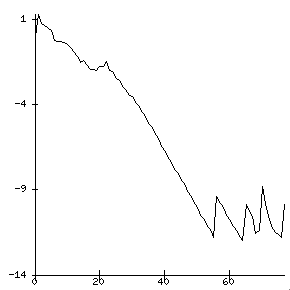
\includegraphics[width=.31\textwidth]{figures/monitor}
  \hfill
  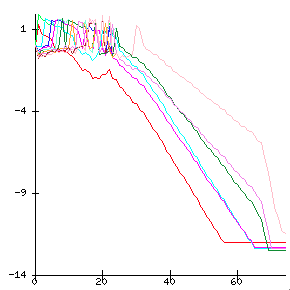
\includegraphics[width=.31\textwidth]{figures/monitorall}
  \hfill
  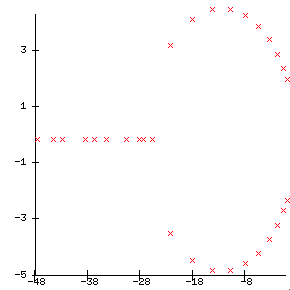
\includegraphics[width=.31\textwidth]{figures/ploteigs}
  \caption{\label{fig:plot}Graphical output in \slepc: default convergence monitor (left), simultaneous convergence monitor for all eigenvalues (middle) and eigenvalue plot (right).}
\end{figure}

	The two previously mentioned monitors have an alternative version (\Verb!*_all!) that processes all eigenvalues instead of just the first one. Figure \ref{fig:plot} (middle) corresponds to the same example but with \Verb!-eps_monitor_draw_all!. Note that these variants have a side effect: they force the computation of all error estimates even if the method would not normally do so. 

	A less verbose textual monitor is \Verb!-eps_monitor_conv!, which simply displays the iteration number at which convergence takes places.
\begin{Verbatim}[fontsize=\footnotesize,numbers=none]
   $ ./ex9 -n 200 -eps_nev 12 -eps_tol 1e-12 -eps_monitor_conv

    56 EPS converged value (error) #0 4.64001e-06+2.13951i (9.82993423e-13)
    56 EPS converged value (error) #1 4.64001e-06-2.13951i (9.82993423e-13)
    65 EPS converged value (error) #2 -0.674926+2.52867i (4.58639033e-13)
    65 EPS converged value (error) #3 -0.674926-2.52867i (4.58639033e-13)
    65 EPS converged value (error) #4 -1.79963+3.03259i (5.24172024e-13)
    65 EPS converged value (error) #5 -1.79963-3.03259i (5.24172024e-13)
    69 EPS converged value (error) #6 -3.37383+3.55626i (3.17374477e-13)
    69 EPS converged value (error) #7 -3.37383-3.55626i (3.17374477e-13)
    70 EPS converged value (error) #8 -5.39714+4.03398i (4.08586434e-13)
    70 EPS converged value (error) #9 -5.39714-4.03398i (4.08586434e-13)
    77 EPS converged value (error) #10 -7.86906+4.41229i (9.08070733e-13)
    77 EPS converged value (error) #11 -7.86906-4.41229i (9.08070733e-13)
\end{Verbatim}

Note that several monitors can be used at the same time.

Finally, the options database key \Verb!-eps_plot_eigs! instructs \slepc to plot the computed approximations of the eigenvalues at the end of the process. See Figure \ref{fig:plot} (right) for an example.

%---------------------------------------------------
\section{Advanced Usage}

	This section includes the description of advanced features of the eigensolver object. Default settings are appropriate for most applications and modification is unnecessary for normal usage.

\subsection{Initial Guesses}

	In this subsection, we consider the possibility of providing initial guesses so that the eigensolver can exploit this information to get the answer faster.

	Most of the algorithms implemented in \ident{EPS} iteratively build and improve a basis of a certain subspace, which will eventually become an eigenspace corresponding to the wanted eigenvalues. In some solvers such as those of Krylov type, this basis is constructed starting from an initial vector, $v_1$, whereas in other solvers such as those of Davidson type, an arbitrary subspace can be used to start the method. By default, \ident{EPS} initializes the starting vector or the initial subspace randomly. This default is a reasonable choice. However, it is also possible to supply an initial subspace with the command
	\findex{EPSSetInitialSpace}
	\begin{Verbatim}[fontsize=\small]
	EPSSetInitialSpace(EPS eps,PetscInt n,Vec *is);
	\end{Verbatim}
In some cases, a suitable initial space can accelerate convergence significantly, for instance when the eigenvalue calculation is one of a sequence of closely related problems, where the eigenspace of one problem is fed as the initial guess for the next problem.

Note that if the eigensolver supports only a single initial vector, but several guesses are provided, then all except the first one will be discarded. One could still build a vector that is rich in the directions of all guesses, by taking a linear combination of them, but this is less effective than using a solver that considers all guesses as a subspace.

In cases where the eigensolver works with two bases, we can think of the second one as containing approximations to the left eigenspace. If initial guesses for the left eigenvectors are available, then one can provide them with
	\findex{EPSSetInitialSpace}
	\begin{Verbatim}[fontsize=\small]
	EPSSetInitialSpaceLeft(EPS eps,PetscInt n,Vec *is);
	\end{Verbatim}

\subsection{Dealing with Deflation Subspaces}

	In some applications, when solving an eigenvalue problem the user wishes to use a priori knowledge about the solution. This is the case when an invariant subspace has already been computed (e.g., in a previous \ident{EPSSolve} call) or when a basis of the null-space is known.

	Consider the following example. Given a graph $G$, with vertex set $V$ and edges $E$, the Laplacian matrix of $G$ is a sparse symmetric positive semidefinite matrix $L$ with elements
$$l_{ij}=\left\{\begin{array}{cl}
         d(v_i) & \mathrm{if}\;i=j\\
         -1 & \mathrm{if}\;e_{ij}\in E\\
         0&\mathrm{otherwise}
\end{array}\right.$$
where $d(v_i)$ is the degree of vertex $v_i$. This matrix is singular since all row sums are equal to zero. The constant vector is an eigenvector with zero eigenvalue, and if the graph is connected then all other eigenvalues are positive. The so-called Fiedler vector is the eigenvector associated to the smallest nonzero eigenvalue and can be used in heuristics for a number of graph manipulations such as partitioning. One possible way of computing this vector with \slepc is to instruct the eigensolver to search for the smallest eigenvalue (with \ident{EPSSetWhichEigenpairs} or by using a spectral transformation as described in next chapter) but preventing it from computing the already known eigenvalue. For this, the user must provide a basis for the invariant subspace (in this case just vector $[1,1,\ldots,1]^T$) so that the eigensolver can \emph{deflate} this subspace. This process is very similar to what eigensolvers normally do with invariant subspaces associated to eigenvalues as they converge. In other words, when a deflation space has been specified, the eigensolver works with the restriction of the problem to the orthogonal complement of this subspace.

	The following function can be used to provide the \ident{EPS} object with some basis vectors corresponding to a subspace that should be deflated during the solution process. 
	\findex{EPSSetDeflationSpace}
	\begin{Verbatim}[fontsize=\small]
	EPSSetDeflationSpace(EPS eps,PetscInt n,Vec *ds)
	\end{Verbatim}
The value \texttt{n} indicates how many vectors are passed in argument \texttt{ds}.

	The deflation space can be any subspace but typically it is most useful in the case of an invariant subspace or a null-space. In any case, \slepc internally checks to see if all (or part of) the provided subspace is a null-space of the associated linear system (see \S\ref{sec:lin}). In this case, this null-space is passed to the linear solver (see \petsc's function \texttt{KSPSetNullSpace}) to enable the solution of singular systems. In practice, this allows the computation of eigenvalues of singular pencils (i.e., when $A$ and $B$ share a common null-space).

\subsection{Orthogonalization}
\label{sec:orthog}

	Internally, eigensolvers in \ident{EPS} often need to orthogonalize a vector against a set of vectors (for instance, when building an orthonormal basis of a Krylov subspace). This operation is carried out typically by a Gram-Schmidt orthogonalization procedure. The user is able to adjust several options related to this algorithm, although the default behavior is good for most cases, and we strongly suggest not to change any of these settings. This topic is covered in detail in \hyperlink{str}{[STR-1]}.

\subsection{Computing a Large Portion of the Spectrum}
\label{sec:large-nev}

We now consider the case when the user requests a relatively large number of eigenpairs (the related case of computing all eigenvalues in a given interval is addressed in \S\ref{sec:slice}). To fix ideas, suppose that the problem size (the dimension of the matrix, denoted as \texttt{n}), is in the order of 100,000's, and the user wants \texttt{nev} to be approximately 5,000 (recall the notation of \ident{EPSSetDimensions} in \S\ref{sec:defprob}).

The first comment is that for such large values of \texttt{nev}, the rule of thumb suggested in \S\ref{sec:defprob} for selecting the value of \texttt{ncv} ($\mathtt{ncv}\geq2\cdot\mathtt{nev}$) may be inappropriate. For small values of \texttt{nev}, this rule of thumb is intended to provide the solver with a sufficiently large subspace. But for large values of \texttt{nev}, it may be enough setting \texttt{ncv} to be slightly larger than \texttt{nev}.

The second thing to take into account has to do with costs, both in terms of storage and in terms of computational effort. This issue is dependent on the particular eigensolver used, but generally speaking the user can simplify to the following points:
\begin{enumerate}
\item It is necessary to store a basis of the subspace, that is, \texttt{ncv} vectors of length \texttt{n}.
\item A considerable part of the computation is devoted to orthogonalization of the basis vectors, whose cost is roughly of order $\mathtt{ncv}^2\cdot\mathtt{n}$.
\item Within the eigensolution process, a projected eigenproblem of order \texttt{ncv} is built. At least one dense matrix of this dimension has to be stored.
\item Solving the projected eigenproblem has a computational cost of order $\mathtt{ncv}^3$. Typically, such problems need to be solved many times within the eigensolver iteration.
\end{enumerate}

It is clear that a large value of \texttt{ncv} implies a high storage requirement (points 1 and 3, especially point 1), and a high computational cost (points 2 and 4, especially point 2). However, in a scenario of such big eigenproblems, it is customary to solve the problem in parallel with many processors. In that case, it turns out that the basis vectors are stored in a distributed way and the associated operations are parallelized, so that points 1 and 2 become benign as long as sufficient processors are used. Then points 3 and 4 become really critical since in the current \slepc version the projected eigenproblem (and its associated operations) are not treated in parallel. In conclusion, the user must be aware that using a large \texttt{ncv} value introduces a serial step in the computation with high cost, that cannot be amortized by increasing the number of processors. 

From \slepc 3.0.0, another parameter \texttt{mpd} has been introduced to alleviate this problem. The name \texttt{mpd} stands for maximum projected dimension. The idea is to bound the size of the projected eigenproblem so that steps 3 and 4 work with a dimension of \texttt{mpd} at most, while steps 1 and 2 still work with a bigger dimension, up to \texttt{ncv}. Suppose we want to compute \texttt{nev}=5000. Setting \texttt{ncv}=10000 or even \texttt{ncv}=6000 would be prohibitively expensive, for the reasons explained above. But if we set e.g. \texttt{mpd}=600 then the overhead of steps 3 and 4 will be considerably diminished. Of course, this reduces the potential of approximation at each outer iteration of the algorithm, but with more iterations the same result should be obtained. The benefits will be specially noticeable in the setting of parallel computation with many processors.

Note that it is not necessary to set both \texttt{ncv} and \texttt{mpd}. For instance, one can do
\begin{Verbatim}[fontsize=\small]
	$ ./program -eps_nev 5000 -eps_mpd 600
\end{Verbatim}

\subsection{Computing Interior Eigenvalues with Harmonic Extraction}
\label{sec:harmonic}

The standard Rayleigh-Ritz projection procedure described in \S\ref{sec:eig} is most appropriate for approximating eigenvalues located at the periphery of the spectrum, especially those of largest magnitude. Most eigensolvers in \slepc are restarted, meaning that the projection is carried out repeatedly with increasingly good subspaces. An effective restarting mechanism, such as that implemented in Krylov-Schur, improves the subspace by realizing a filtering effect that tries to eliminate components in the direction of unwanted eigenvectors. In that way, it is possible to compute eigenvalues located anywhere in the spectrum, even in its interior.

Even though in theory eigensolvers could be able to approximate interior eigenvalues with a standard extraction technique, in practice convergence difficulties may arise that prevent success. The problem comes from the property that Ritz values (the approximate eigenvalues provided by the standard projection procedure) converge from the interior to the periphery of the spectrum. That is, the Ritz values that stabilize first are those in the periphery, so convergence of interior ones requires the previous convergence of all eigenvalues between them and the periphery. Furthermore, this convergence behaviour usually implies that restarting is carried out with bad approximations, so the restart is ineffective and global convergence is severely damaged.

Harmonic projection is a variation that uses a target value, $\tau$, around which the user wants to compute eigenvalues (see, e.g., \citep{Morgan:2006:HRA}). The theory establishes that harmonic Ritz values converge in such a way that eigenvalues closest to the target stabilize first, and also that no unconverged value is ever close to the target, so restarting is safe in this case. As a conclusion, eigensolvers with harmonic extraction may be effective in computing interior eigenvalues. Whether it works or not in practical cases depends on the particular distribution of the spectrum.

In order to use harmonic extraction in \slepc, it is necessary to indicate it explicitly, and provide the target value as described in \S\ref{sec:defprob} (default is $\tau=0$). The type of extraction can be set with:
	\findex{EPSSetExtraction}
	\begin{Verbatim}[fontsize=\small]
	EPSSetExtraction(EPS eps,EPSExtraction extr);
	\end{Verbatim}
Available possibilities are \texttt{EPS\_RITZ} for standard projection and \texttt{EPS\_HARMONIC} for harmonic projection (other alternatives such as refined extraction are still experimental).

A command line example would be:
	\begin{Verbatim}[fontsize=\small]
	$ ./ex5 -m 45 -eps_harmonic -eps_target 0.8 -eps_ncv 60
	\end{Verbatim}
The example computes the eigenvalue closest to $\tau=0.8$ of a real non-symmetric matrix of order 1035. Note that \texttt{ncv} has been set to a larger value than would be necessary for computing the largest magnitude eigenvalues. In general, users should expect a much slower convergence when computing interior eigenvalues compared to extreme eigenvalues. Increasing the value of \texttt{ncv} may help.

Currently, harmonic extraction is available in the default \ident{EPS} solver, that is, Krylov-Schur, and also in Arnoldi, GD, and JD.

\subsection{Balancing for Non-Hermitian Problems}
\label{sec:balancing}

In problems where the matrix has a large norm, $\|A\|_2$, the roundoff errors introduced by the eigensolver may be large. The goal of balancing is to apply a simple similarity transformation, $DAD^{-1}$, that keeps the eigenvalues unaltered but reduces the matrix norm, thus enhancing the accuracy of the computed eigenpairs. Obviously, this makes sense only in the non-Hermitian case. The matrix $D$ is chosen to be diagonal, so balancing amounts to scaling the matrix rows and columns appropriately.

In \slepc, the matrix $DAD^{-1}$ is not formed explicitly. Instead, the operators of Table \ref{tab:op} are preceded by a multiplication by $D^{-1}$ and followed by a multiplication by $D$. This allows for balancing in the case of problems with an implicit matrix.

A simple and effective Krylov balancing technique, described in \citep{Chen:2000:BSM}, is implemented in \slepc. The user calls the following subroutine to activate it.
	\findex{EPSSetBalance}
	\begin{Verbatim}[fontsize=\small]
	EPSSetBalance(EPS eps,EPSBalance bal,PetscInt its,PetscReal cutoff);
	\end{Verbatim}
Two variants are available, one-sided and two-sided, and there is also the possibility for the user to provide a pre-computed $D$ matrix.

%-------------------------------------------------------
% SLEPc Users Manual
%-------------------------------------------------------
\chapter{\label{cap:st}ST: Spectral Transformation}
%-------------------------------------------------------

\noindent The Spectral Transformation (\ident{ST}) is the object that encapsulates the functionality required for acceleration techniques based on the transformation of the spectrum. Most eigensolvers in \ident{EPS} work by applying an operator to a set of vectors and this operator can adopt different forms. The \ident{ST} object handles all the different possibilities in a uniform way, so that the solver can proceed without knowing which transformation has been selected. The spectral transformation can be specified at run time, as well as related options such as which linear solver to use.

	Despite being a rather unrelated concept, \ident{ST} is also used to handle the preconditioners and correction-equation solvers used in preconditioned eigensolvers such as GD and JD.

	The description in this chapter focuses on the use of \ident{ST} in the context of \ident{EPS}. For usage within other solver classes, we will provide further details, e.g., shift-and-invert for polynomial eigenproblems in \S\ref{sec:qst}.

%---------------------------------------------------
\section{General Description}

	Spectral transformations are powerful tools for adjusting the way in which eigensolvers behave when coping with a problem. The general strategy consists in transforming the original problem into a new one in which eigenvalues are mapped to a new position while eigenvectors remain unchanged. These transformations can be used with several goals in mind:
\begin{itemize}
\setlength{\itemsep}{-2pt}
\item Compute internal eigenvalues. In some applications, the eigenpairs of interest are not the extreme ones (largest magnitude, smallest magnitude, rightmost, leftmost), but those contained in a certain interval or those closest to a certain value of the complex plane.
\item Accelerate convergence. Convergence properties typically depend on how close the eigenvalues are from each other. With some spectral transformations, difficult eigenvalue distributions can be remapped in a more favorable way in terms of convergence.
\item Handle some special situations. For instance, in generalized problems when matrix $B$ is singular, it may be necessary to use a spectral transformation.
\end{itemize}
	
	\slepc separates spectral transformations from solution methods so that any combination of them can be specified by the user. To achieve this, most eigensolvers contained in \ident{EPS} are implemented in such a way that they are independent of which transformation has been selected by the user (the exception are preconditioned solvers, see below). That is, the solver algorithm has to work with a generic operator, whose actual form depends on the transformation used. After convergence, eigenvalues are transformed back appropriately.

	For technical details of the transformations described in this chapter, the interested user is referred to \citep{Ericsson:1980:STL}, \citep{Scott:1982:AIO}, \citep{Nour-Omid:1987:HIS}, and \citep{Meerbergen:1994:SCT}.

\paragraph{Preconditioners.}

As explained in the previous chapter, \ident{EPS} contains preconditioned eigensolvers such as GD or JD. These solvers either apply a preconditioner at a certain step of the computation, or need to solve a correction equation with a preconditioned linear solver. One of the main goals of these solvers is to achieve a similar effect as an inverse-based spectral transformation such as shift-and-invert, but with less computational cost. For this reason, a ``preconditioner'' spectral transformation has been included in the \ident{ST} object. However, this is just a convenient way of organizing the functionality, since this fake spectral transform cannot be used with non-preconditioned eigensolvers, and conversely preconditioned eigensolvers cannot be used with conventional spectral transformations.

%---------------------------------------------------
\section{Basic Usage}

	The \ident{ST} module is the analog of some \petsc modules such as \texttt{PC}. The user does not usually need to create a stand-alone \ident{ST} object explicitly. Instead, every \ident{EPS} object internally sets up an associated \ident{ST}. Therefore, the usual object management methods such as \ident{STCreate}, \ident{STDestroy}, \ident{STView}, \ident{STSetFromOptions}, are not usually called by the user.

	Although the \ident{ST} context is hidden inside the \ident{EPS} object, the user still has control over all the options, by means of the command line, or also inside the program. To allow application programmers to set any of the spectral transformation options directly within the code, the following routine is provided to extract the \ident{ST} context from the \ident{EPS} object,
	\findex{EPSGetST}
	\begin{Verbatim}[fontsize=\small]
	EPSGetST(EPS eps,ST *st);
	\end{Verbatim}
	
	After this, one is able to set any options associated with the \ident{ST} object. For example, to set the value of the shift, the following function is available
	\findex{STSetShift}
	\begin{Verbatim}[fontsize=\small]
	STSetShift(ST st,PetscScalar shift);
	\end{Verbatim}
	This can also be done with the command line option \Verb!-st_shift <shift>!. Note that the argument \texttt{shift} is defined as a \texttt{PetscScalar}, and this means that complex shifts are not allowed unless the complex version of \slepc is used.

	Other object operations are available, which are not usually called by the user. The most important of such functions are \ident{STApply}, which applies the operator to a vector, and \ident{STSetUp}, which prepares all the necessary data structures before the solution process starts. The term ``operator'' refers to one of $A$, $B^{-1}\!A$, $A-\sigma I$, ...\ depending on which kind of spectral transformation is being used.

%---------------------------------------------------
\section{Available Transformations}

	This section describes the spectral transformations that are provided in \slepc. As in the case of eigensolvers, the spectral transformation to be used can be specified procedurally or via the command line. The application programmer can set it by means of the command
	\findex{STSetType}
	\begin{Verbatim}[fontsize=\small]
	STSetType(ST st,STType type);
	\end{Verbatim}
where \texttt{type} can be one of
\texttt{STSHIFT},
\texttt{STSINVERT}, \texttt{STCAYLEY},
\texttt{STPRECOND}, or \texttt{STSHELL}.
The \ident{ST} type can also be set with the command-line option \Verb!-st_type! followed by the name of the method (see Table \ref{tab:transforms}). The first four spectral transformations are described in detail in the rest of this section. The last possibility, \texttt{STSHELL}, uses a specific, application-provided spectral transformation. Section \ref{sec:shell} describes how to implement one of these transformations.

\begin{table}
\centering
{\small \begin{tabular}{lllc}
                        &                   & {\footnotesize Options} &\\
Spectral Transformation & \ident{STType}    & {\footnotesize Name}    & Operator\\\hline
Shift of Origin         & \texttt{STSHIFT}  & \texttt{shift}   & $B^{-1}A-\sigma I$\\
Shift-and-invert        & \texttt{STSINVERT}& \texttt{sinvert} & $(A-\sigma B)^{-1}B$\\
Generalized Cayley      & \texttt{STCAYLEY} & \texttt{cayley}  & $(A-\sigma B)^{-1}(A+\nu B)$\\
Preconditioner          & \texttt{STPRECOND}& \texttt{precond} & $K^{-1}\approx(A-\sigma B)^{-1}$\\\hline
Shell Transformation    & \texttt{STSHELL}  & \texttt{shell}   & \emph{user-defined}\\\hline
\end{tabular} }
\caption{\label{tab:transforms}Spectral transformations available in the  \ident{ST} package.}
\end{table}

	The last column of Table \ref{tab:transforms} shows a general form of the operator used in each case. This generic operator can adopt different particular forms depending on whether the eigenproblem is standard or generalized, or whether the value of the shift ($\sigma$) and anti-shift ($\nu$) is zero or not. All the possible combinations are listed in Table \ref{tab:op}.
	\begin{table}
	\centering
	{\small \begin{tabular}{llcc}
	\ident{ST}     & Choice of $\sigma,\nu$ & Standard problem & Generalized problem \\\hline
	\texttt{shift}
        & $\sigma=0$     & $A$           & $B^{-1}A$          \\
	& $\sigma\not=0$ & $A-\sigma I$  & $B^{-1}A-\sigma I$ \\ \hline
	\texttt{sinvert}
        & $\sigma=0$     & $A^{-1}$      & $A^{-1}B$          \\
	& $\sigma\not=0$ & $(A-\sigma I)^{-1}$  & $(A-\sigma B)^{-1}B$ \\ \hline
	\texttt{cayley}
	& $\sigma\not=0,\nu=0$ & $(A-\sigma I)^{-1}A$  & $(A-\sigma B)^{-1}A$ \\
        & $\sigma=0,\nu\not=0$     & $I+\nu A^{-1}$      & $I+\nu A^{-1}B$ \\
	& $\sigma\not=0,\nu\not=0$ & $(A-\sigma I)^{-1}(A+\nu I)$  & $(A-\sigma B)^{-1}(A+\nu B)$ \\ \hline
	\texttt{precond}
        & $\sigma=0$     & $K^{-1}\approx A^{-1}$ & $K^{-1}\approx A^{-1}$          \\
	& $\sigma\not=0$ & $K^{-1}\approx(A-\sigma I)^{-1}$ & $K^{-1}\approx(A-\sigma B)^{-1}$ \\ \hline
	\end{tabular} }
	\caption{\label{tab:op}Operators used in each spectral transformation mode.}
	\end{table}

	The expressions shown in Table \ref{tab:op} are not built explicitly. Instead, the appropriate operations are carried out when applying the operator to a certain vector. The inverses imply the solution of a linear system of equations that is managed by setting up an associated \ident{KSP} object. The user can control the behavior of this object by adjusting the appropriate options, as will be illustrated with examples in \S\ref{sec:lin}.

\paragraph{Relation between Target and Shift.}

	In all transformations except \ident{STSHIFT}, there is a direct connection between the target $\tau$ (described in \S\ref{sec:defprob}) and the shift $\sigma$, as will be discussed below. The normal usage is that the user sets the target and then $\sigma$ is set to $\tau$ automatically (though it is still possible for the user to set a different value of the shift).

\subsection{Shift of Origin}

	By default, no spectral transformation is performed. This is equivalent to a shift of origin (\texttt{STSHIFT}) with $\sigma=0$, that is, the first line of Table \ref{tab:op}. The solver works with the original expressions of the eigenvalue problems,
\begin{equation}Ax=\lambda x,\end{equation}
for standard problems, and $Ax=\lambda Bx$ for generalized ones. Note that this last equation is actually treated internally as
\begin{equation}B^{-1}Ax=\lambda x.\end{equation}
When the eigensolver in \ident{EPS} requests the application of the operator to a vector, a matrix-vector multiplication by matrix $A$ is carried out (in the standard case) or a matrix-vector multiplication by matrix $A$ followed by a linear system solve with coefficient matrix $B$ (in the generalized case). Note that in the last case, the operation will fail if matrix $B$ is singular.

When the shift, $\sigma$, is given a value different from the default, 0, the effect is to move the whole spectrum by that exact quantity, $\sigma$, which is called \emph{shift of origin}. To achieve this, the solver works with the shifted matrix, that is, the expressions it has to cope with are
\begin{equation}(A-\sigma I)x=\theta x,\end{equation}
for standard problems, and
\begin{equation}(B^{-1}A-\sigma I) x=\theta x,\end{equation}
for generalized ones. The important property that is used is that shifting does not alter the eigenvectors and that it does change the eigenvalues in a simple known way, it shifts them by $\sigma$. In both the standard and the generalized problems, the following relation holds
\begin{equation}\theta=\lambda-\sigma.\end{equation}
This means that after the solution process, the value $\sigma$ has to be added\footnote{Note that the sign changed in \slepc 3.5 with respect to previous versions.} to the computed eigenvalues, $\theta$, in order to retrieve the solution of the original problem, $\lambda$. This is done by means of the function \ident{STBackTransform}, which does not need to be called directly by the user.

\subsection{Shift-and-invert}

  \begin{figure}[t]
    \centering
    \begin{tikzpicture}
      \draw[->] (-1.5,0) -- (5.5,0) node[right] {$\lambda$};
      \draw[->] (0,-4) -- (0,4) node[above] {$\theta$};
      \draw[dashed,color=gray] (2,-4) -- (2,4);
      %\draw[color=blue] plot[id=sinv1,domain=-1.3:1.75] function{1/(x-2)};
      \draw[color=blue]
        (-1.30000,-0.30303) -- (-1.17292,-0.31517) -- (-1.04583,-0.32832) --
        (-0.91875,-0.34261) -- (-0.79167,-0.35821) -- (-0.66458,-0.37529) --
        (-0.53750,-0.39409) -- (-0.41042,-0.41487) -- (-0.28333,-0.43796) --
        (-0.15625,-0.46377) -- (-0.02917,-0.49281) -- ( 0.09792,-0.52574) --
        ( 0.22500,-0.56338) -- ( 0.35208,-0.60683) -- ( 0.47917,-0.65753) --
        ( 0.60625,-0.71749) -- ( 0.73333,-0.78947) -- ( 0.86042,-0.87751) --
        ( 0.98750,-0.98765) -- ( 1.11458,-1.12941) -- ( 1.24167,-1.31868) --
        ( 1.36875,-1.58416) -- ( 1.49583,-1.98347) -- ( 1.62292,-2.65193) --
        ( 1.75000,-4.00000);
      %\draw[color=blue] plot[id=sinv2,domain=2.25:5.3] function{1/(x-2)};
      \draw[color=blue]
        (2.25000,4.00000) -- (2.37708,2.65193) -- (2.50417,1.98347) --
        (2.63125,1.58416) -- (2.75833,1.31868) -- (2.88542,1.12941) --
        (3.01250,0.98765) -- (3.13958,0.87751) -- (3.26667,0.78947) --
        (3.39375,0.71749) -- (3.52083,0.65753) -- (3.64792,0.60683) --
        (3.77500,0.56338) -- (3.90208,0.52574) -- (4.02917,0.49281) --
        (4.15625,0.46377) -- (4.28333,0.43796) -- (4.41042,0.41487) --
        (4.53750,0.39409) -- (4.66458,0.37529) -- (4.79167,0.35821) --
        (4.91875,0.34261) -- (5.04583,0.32832) -- (5.17292,0.31517) --
        (5.30000,0.30303);
      \node[below right] at (0,0) {$0$};
      \draw (2,0.1) -- (2,-0.1) node[below left] at (2,0) {$\sigma$};
      \node at (4,3.2) {$\theta = \frac{1}{\lambda-\sigma}$};
      \draw[very thin,color=gray] (2.5,0) |- (0,2);
      \draw[very thin,color=gray] (3.9,0) |- (0,0.5263);
      \foreach \pos/\label in {2/$\theta_1$,0.5263/$\theta_2$}
      \draw (-0.1,\pos) -- (0.1,\pos) (-0.8mm,\pos cm) node[anchor=east,font=\footnotesize] {\label};
      \foreach \pos/\label in {2.5/$\lambda_1$,3.9/$\lambda_2$}
      \draw (\pos,0.1) -- (\pos,-0.1) (\pos cm,-2.5ex) node[anchor=base,font=\footnotesize] {\label};
    \end{tikzpicture}
    \caption{\label{fig:sinvert}The shift-and-invert spectral transformation.}
  \end{figure}

	The shift-and-invert spectral transformation (\texttt{STSINVERT}) is used to enhance convergence of eigenvalues in the neighborhood of a given value. In this case, the solver deals with the expressions
\begin{eqnarray}
(A-\sigma I)^{-1}x=\theta x,\\
(A-\sigma B)^{-1}B x=\theta x,
\end{eqnarray}
for standard and generalized problems, respectively.
This transformation is effective for finding eigenvalues near $\sigma$ since the eigenvalues $\theta$ of the operator that are largest in magnitude correspond to the eigenvalues $\lambda$ of the original problem that are closest to the shift $\sigma$ in absolute value, as illustrated in Figure \ref{fig:sinvert} for an example with real eigenvalues. Once the wanted eigenvalues have been found, they may be transformed back to eigenvalues of the original problem. Again, the eigenvectors remain unchanged.
In this case, the relation between the eigenvalues of both problems is
\begin{equation}\theta=1/(\lambda-\sigma).\end{equation}
Therefore, after the solution process, the operation to be performed in function \ident{STBackTransform} is $\lambda=\sigma+1/\theta$ for each of the computed eigenvalues.

This spectral transformation is used in the spectrum slicing technique, see \S\ref{sec:slice}.

\subsection{Cayley}
\label{sec:cayley}

	The generalized Cayley transform (\texttt{STCAYLEY}) is defined from the expressions
\begin{eqnarray}
(A-\sigma I)^{-1}(A+\nu I)x=\theta x,\\
(A-\sigma B)^{-1}(A+\nu B)x=\theta x,
\end{eqnarray}
for standard and generalized problems, respectively. Sometimes, the term Cayley transform is applied for the particular case in which $\nu=\sigma$. This is the default if $\nu$ is not given a value explicitly. The value of $\nu$ (the anti-shift) can be set with the following function
	\findex{STCayleySetAntishift}
	\begin{Verbatim}[fontsize=\small]
	STCayleySetAntishift(ST st,PetscScalar nu);
	\end{Verbatim}
or in the command line with \Verb!-st_cayley_antishift!.

This transformation is mathematically equivalent to shift-and-invert and, therefore, it is effective for finding eigenvalues near $\sigma$ as well. However, in some situations it is numerically advantageous with respect to shift-and-invert (see \citep[\S 11.2]{Bai:2000:TSA}, \citep{Lehoucq:2001:LEC}).

In this case, the relation between the eigenvalues of both problems is
\begin{equation}\theta=(\lambda+\nu)/(\lambda-\sigma).\end{equation}
Therefore, after the solution process, the operation to be performed in function \ident{STBackTransform} is $\lambda=(\theta\sigma+\nu)/(\theta-1)$ for each of the computed eigenvalues.

\subsection{Preconditioner}
\label{sec:precond}

	As mentioned in the introduction of this chapter, the special type \ident{STPRECOND} is used for handling preconditioners or preconditioned iterative linear solvers, which are used in the context of preconditioned eigensolvers for expanding the subspace. For instance, in the GD solver the so-called correction vector $d_i$ to be added to the subspace in each iteration is computed as
\begin{equation}
d_i=K^{-1}P_i(A-\theta_i B)x_i,
\end{equation}
where $(\theta_i,x_i)$ is the current approximation of the sought-after eigenpair, and $P_i$ is a projector involving $x_i$ and $K^{-1}x_i$. In the above expressions, $K$ is a preconditioner matrix that is built from $A-\theta_i B$. However, since $\theta_i$ changes at each iteration, which would force recomputation of the preconditioner, we opt for using
\begin{equation}
\label{eq:precon}
K^{-1}\approx (A-\sigma B)^{-1}.
\end{equation}

	Similarly, in the JD eigensolver the expansion of the subspace is carried out by solving a correction equation similar to
\begin{equation}
(I-x_ix_i^*)(A-\theta_i B)(I-x_ix_i^*)d_i=-(A-\theta_i B)x_i,
\end{equation}
where the system is solved approximately with a preconditioned iterative linear solver. For building the preconditioner of this linear system, the projectors $I-x_ix_i^*$ are ignored, and again it is not recomputed in each iteration. Therefore, the preconditioner is built as in expression \ref{eq:precon} as well.

	It should be clear from the previous discussion, that \ident{STPRECOND} does not work in the same way as the rest of spectral transformations. In particular, it is not intended to be used on the basis of operator applications with \ident{STApply}, and it does not rely on \ident{STBackTransform} either. It is rather a convenient mechanism for handling the preconditioner and linear solver (see examples in \S\ref{sec:lin}). The expressions shown in Tables \ref{tab:transforms} and \ref{tab:op} are just a reference to indicate from which matrix the preconditioner is built by default.

	There is the possibility that the user overrides the default behaviour, that is, to explicitly supply a matrix from which the preconditioner is to be built, with
	\findex{STPrecondSetMatForPC}
	\begin{Verbatim}[fontsize=\small]
	STPrecondSetMatForPC(ST st,Mat mat);
	\end{Verbatim}

	Note that preconditioned eigensolvers in \ident{EPS} select \ident{STPRECOND} by default, so the user does not need to specify it explicitly.

%---------------------------------------------------
\section{Advanced Usage}

Using the \ident{ST} object is very straightforward. However, when using spectral transformations many things are happening behind the scenes, mainly the solution of linear systems of equations. The user must be aware of what is going on in each case, so that it is possible to guide the solution process in the most beneficial way. This section describes several advanced aspects that can have a considerable impact on efficiency.

\subsection{Solution of Linear Systems}
\label{sec:lin}

	In many of the cases shown in Table \ref{tab:op}, the operator contains an inverted matrix, which means that a linear system of equations must be solved whenever the application of the operator to a vector is required. These cases are handled internally by means of a \ident{KSP} object.

	In the simplest case, a generalized problem is to be solved with a zero shift. Suppose you run a program that solves a generalized eigenproblem, with default options:
\begin{Verbatim}[fontsize=\small]
	$ ./program
\end{Verbatim}
In this case, the \ident{ST} object associated with the \ident{EPS} solver creates a \ident{KSP} object whose coefficient matrix is $B$. By default, this \ident{KSP} object is set to use a direct solver\footnote{This is the default since \slepc 3.0.0.}, in particular an LU factorization. However, default settings can be changed, as illustrated below.

	The following command-line is equivalent to the previous one:
\begin{Verbatim}[fontsize=\small]
	$ ./program -st_ksp_type preonly -st_pc_type lu
\end{Verbatim}
The two options specify the type of the linear solver and preconditioner to be used. The \Verb!-st_! prefix indicates that the option corresponds to the linear solver within \ident{ST}. The combination \texttt{preonly}$+$\texttt{lu} instructs to use a direct solver (LU factorization, see \petsc's documentation for details), so this is the same as the default. Adding a new option changes the default behaviour, for instance
\begin{Verbatim}[fontsize=\small]
	$ ./program -st_ksp_type preonly -st_pc_type lu
                    -st_pc_factor_mat_solver_package mumps
\end{Verbatim}
In this case, an external linear solver package is used (MUMPS, see \petsc's documentation for other available packages). Note that an external package is required for computing a matrix factorization in parallel, since \petsc itself only provides sequential direct linear solvers.

	Instead of a direct linear solver, it is possible to use an iterative solver. This may be necessary in some cases, specially for very large problems. However, the user is warned that using an iterative linear solver makes the overall solution process less robust (see also the discussion of preconditioned eigensolvers below). As an example, the command-line
\begin{Verbatim}[fontsize=\small]
	$ ./program -st_ksp_type gmres -st_pc_type bjacobi -st_ksp_rtol 1e-9
\end{Verbatim}
selects the GMRES solver with block Jacobi preconditioning. In the case of iterative solvers, it is important to use an appropriate tolerance, usually slightly more stringent for the linear solves relative to the desired accuracy of the eigenvalue calculation ($10^{-9}$ in the example, compared to $10^{-8}$ for the eigensolver).

	Although the direct solver approach may seem too costly, note that the factorization is only carried out at the beginning of the eigenvalue calculation and this cost is amortized in each subsequent application of the operator. This is also the case for iterative methods with preconditioners with high-cost set-up such as ILU.

	The application programmer is able to set the desired linear systems solver options also from within the code. In order to do this, first the context of the \ident{KSP} object must be retrieved with the following function
	\findex{STGetKSP}
	\begin{Verbatim}[fontsize=\small]
	STGetKSP(ST st,KSP *ksp);
	\end{Verbatim}
	
	The above functionality is also applicable to the other spectral transformations. For instance, for the shift-and-invert technique with $\tau=10$ using BiCGStab+Jacobi:
\begin{Verbatim}[fontsize=\small]
	$ ./program -st_type sinvert -eps_target 10 -st_ksp_type bcgs -st_pc_type jacobi
\end{Verbatim}
	In shift-and-invert and Cayley, unless $\sigma=0$, the coefficient matrix is not a simple matrix but an expression that can be explicitly constructed or not, depending on the user's choice. This issue is examined in detail in \S\ref{sec:explicit} below.

In many cases, especially if a shift-and-invert or Cayley transformation is being used, iterative methods may not be well suited for solving linear systems (because of the properties of the coefficient matrix that can be indefinite and ill-conditioned). When using an iterative linear solver, it may be helpful to run with the option \Verb!-st_ksp_converged_reason!, which will display the number of iterations required in each operator application.
In extreme cases, the iterative solver fails, so \ident{EPSSolve} aborts with an error
\begin{Verbatim}[fontsize=\small]
	[0]PETSC ERROR: KSP did not converge (reason=DIVERGED_ITS)!
\end{Verbatim}
If this happens, it is necessary to use a direct method for solving the linear systems, as explained above.

\paragraph{The Case of Preconditioned Eigensolvers.}

	The \texttt{KSP} object contained internally in \ident{ST} is also used for applying the preconditioner or solving the correction equation in preconditioned eigensolvers.

	The GD eigensolver employs just a preconditioner. Therefore, by default it sets the \texttt{KSP} type to \texttt{preonly} (no other \texttt{KSP} is allowed) and the \texttt{PC} type to \texttt{jacobi}. The user may change the preconditioner, for example as
\begin{Verbatim}[fontsize=\small]
	$ ./ex5 -eps_type gd -st_pc_type asm
\end{Verbatim}

	The JD eigensolver uses both an iterative linear solver and a preconditioner, so both \texttt{KSP} and \texttt{PC} are meaningful in this case. The default is \texttt{gmres}+\texttt{bjacobi}. It is important to note that, contrary to the ordinary spectral transformations where a direct linear solver is recommended, in JD using an iterative linear solver is usually better than a direct solver. Indeed, the best performance may be achieved with a few iterations of the linear solver (or a large tolerance). For instance, the next example uses JD with GMRES+Jacobi limiting to 10 the number of allowed iterations for the linear solver:
\begin{Verbatim}[fontsize=\small]
	$ ./ex5 -eps_type jd -st_ksp_type gmres -st_pc_type jacobi -st_ksp_max_it 10
\end{Verbatim}
A discussion on the different options available for the Davidson solvers can be found in \citep{Romero:2014:PID}.

\subsection{Explicit Computation of Coefficient Matrix}
\label{sec:explicit}

	Three possibilities can be distinguished regarding the form of the coefficient matrix of the linear systems of equations associated with the different spectral transformations. The possible coefficient matrices are:
	\begin{itemize}
	\item Simple: $B$.
	\item Shifted: $A-\sigma I$.
	\item Axpy: $A-\sigma B$.
	\end{itemize}
	The first case has already been described and presents no difficulty. In the other two cases, there are three possible approaches:
	\begin{description}
	\item[``\Verb!shell!''] To work with the corresponding expression without forming the matrix explicitly. This is achieved by internally setting a matrix-free matrix with \ident{MatCreateShell}.
	\item[``\Verb!inplace!''] To build the coefficient matrix explicitly. This is done by means of a \ident{MatShift} or a \ident{MatAXPY} operation, which overwrites matrix $A$ with the corresponding expression. This alteration of matrix $A$ is reversed after the eigensolution process has finished.
	\item[``\Verb!copy!''] To build the matrix explicitly, as in the previous option, but using a working copy of the matrix, that is, without modifying the original matrix $A$.
	\end{description}
	The default behavior is to build the coefficient matrix explicitly in a copy of $A$ (option ``\Verb!copy!''). The user can change this as in the following example
\begin{Verbatim}[fontsize=\small]
	$ ./program -st_type sinvert -eps_target 10 -st_ksp_type cg
                    -st_pc_type jacobi -st_matmode shell
\end{Verbatim}
	As always, the procedural equivalent is also available for specifying this option in the code of the program:
	\findex{STSetMatMode}
	\begin{Verbatim}[fontsize=\small]
	STSetMatMode(ST st,STMatMode mode);
	\end{Verbatim}

	The user must consider which approach is the most appropriate for the particular application. The different options have advantages and drawbacks. The first approach is the simplest one but severely restricts the number of possibilities available for solving the system, in particular most of the \petsc{} preconditioners would not be available, including direct methods. The only preconditioners that can be used in this case are Jacobi (only if matrices $A$ and $B$ have the operation \ident{MATOP\_GET\_DIAGONAL}) or a user-defined one.
	
	The second approach (``\Verb!inplace!'') can be much faster, specially in the generalized case. A more important advantage of this approach is that, in this case, the linear system solver can be combined with any of the preconditioners available in \petsc, including those which need to access internal matrix data-structures such as ILU. The main drawback is that, in the generalized problem, this approach probably makes sense only in the case that $A$ and $B$ have the same sparse pattern, because otherwise the function \ident{MatAXPY} might be inefficient.
If the user knows that the pattern is the same (or a subset), then this can be specified with the function
	\findex{STSetMatStructure}
	\begin{Verbatim}[fontsize=\small]
	STSetMatStructure(ST st,MatStructure str);
	\end{Verbatim}
	
	Note that when the value of the shift $\sigma$ is very close to an eigenvalue, then the linear system will be ill-conditioned and using iterative methods may be problematic. On the other hand, in symmetric definite problems, the coefficient matrix will be indefinite whenever $\sigma$ is a point in the interior of the spectrum.

	The third approach (``\Verb!copy!'') uses more memory but avoids a potential problem that could appear in the ``\Verb!inplace!'' approach: the recovered matrix might be slightly different from the original one (due to roundoff).

\subsection{Preserving the Symmetry in Generalized Eigenproblems}
\label{sec:symm}

	As mentioned in \S\ref{sec:defprob}, some eigensolvers can exploit symmetry and compute a solution for Hermitian problems with less storage and/or computational cost than other methods. Also, symmetric solvers can be more accurate in some cases. However, in the case of generalized eigenvalue problems in which both $A$ and $B$ are symmetric, it happens that, due to the spectral transformation, symmetry is lost since none of the transformed operators $B^{-1}\!A-\sigma I$, $(A-\sigma B)^{-1}B$, etc.\ is symmetric (the same applies in the Hermitian case for complex matrices).

	The solution proposed in \slepc is based on selecting different kinds of inner products. Currently, we have the following choice of inner products:
  \begin{itemize}\setlength{\itemsep}{0pt}
    \item Standard Hermitian inner product: $\langle x,y\rangle=x^*y$.
    \item $B$-inner product: $\langle x,y\rangle_B=x^*\!B\,y$.
  \end{itemize}

	The second one can be used for preserving the symmetry in symmetric definite generalized problems, as described below. Note that $\langle x,y\rangle_B$ is a genuine inner product only if $B$ is symmetric positive definite (for the case of symmetric positive semi-definite $B$ see \S\ref{sec:purif}).

	It can be shown that $\mathbb{R}^n$ with the $\langle x,y\rangle_B$ inner product is isomorphic to the Euclidean $n$-space $\mathbb{R}^n$ with the standard Hermitian inner product. This means that if we use $\langle x,y\rangle_B$ instead of the standard inner product, we are just changing the way lengths and angles are measured, but otherwise all the algebraic properties are maintained and therefore algorithms remain correct. What is interesting to observe is that the transformed operators such as $B^{-1}\!A$ or $(A-\sigma B)^{-1}B$ are self-adjoint with respect to $\langle x,y\rangle_B$.

\begin{figure}
\centering
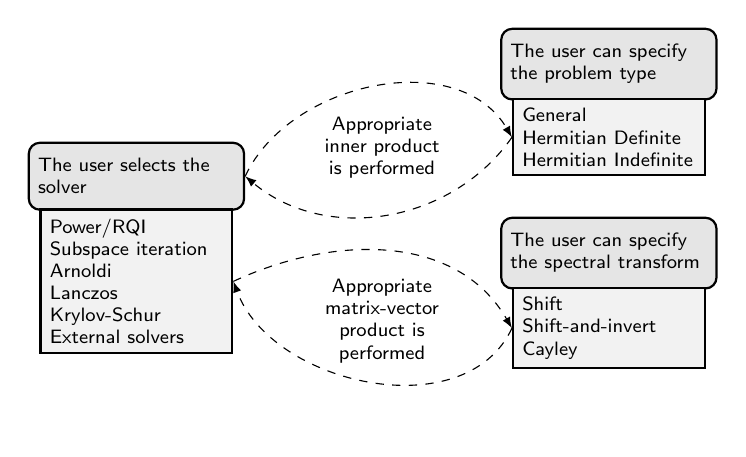
\begin{tikzpicture}
  \begin{scope}[every node/.style={draw,thick,text ragged,font=\sffamily\scriptsize},every to/.style={draw,-stealth,very thick,dashed}]
  \node[above right,rounded corners,fill=black!10,text width=2.5cm,inner ysep=2mm] (n1c) at (0,0)
       {The user selects the solver};
  \node[below right,fill=black!5,text width=2.2cm] (n1) at (0.15,0.03)
       {\begin{minipage}{\textwidth}Power/RQI\\Subspace iteration\\Arnoldi\\Lanczos\\
       Krylov-Schur\\External solvers\end{minipage}};
  \node[above right,rounded corners,fill=black!10,text width=2.5cm,inner ysep=2mm] (n2c) at (6,1.4)
       {The user can specify the problem type};
  \node[below right,fill=black!5,text width=2.2cm] (n2) at (6.15,1.43)
       {\begin{minipage}{\textwidth}General\\Hermitian Definite\\Hermitian Indefinite
       \end{minipage}};
  \node[above right,rounded corners,fill=black!10,text width=2.5cm,inner ysep=2mm] (n3c) at (6,-1.0)
       {The user can specify the spectral transform};
  \node[below right,fill=black!5,text width=2.2cm] (n3) at (6.15,-0.97)
       {\begin{minipage}{\textwidth}Shift\\Shift-and-invert\\Cayley
       \end{minipage}};
  \draw[dashed,-latex] (n1c.east) to[out=65,in=120] (n2.west);
  \draw[dashed,-latex] (n2.west) to[out=-125,in=-40] (n1c.east);
  \draw[dashed,-latex] (n1.east) to[out=25,in=120] (n3.west);
  \draw[dashed,-latex] (n3.west) to[out=-115,in=-70] (n1.east);
  \end{scope}
  \begin{scope}[every node/.style={text centered,text width=2cm,font=\sffamily\scriptsize}]
  \node at (4.5,.8) {Appropriate inner product is performed};
  \node at (4.5,-1.4) {Appropriate matrix-vector product is performed};
  \end{scope}
\end{tikzpicture}
\caption{\label{fig:abstr}Abstraction used by \slepc solvers.}
\end{figure}

	Internally, \slepc operates with the abstraction illustrated in Figure \ref{fig:abstr}. The operations indicated by dashed arrows are implemented as virtual functions. From the user point of view, all the above explanation is transparent. The only thing he/she has to care about is to set the problem type appropriately with \ident{EPSSetProblemType} (see \S\ref{sec:defprob}).
	In the case of the Cayley transform, \slepc is using $\langle x,y\rangle_{A+\nu B}$ as the inner product for preserving symmetry.

	Using the $B$-inner product may be attractive also in the non-symmetric case ($A$ non-symmetric) as described in the next subsection.

	Note that the above discussion is not directly applicable to \ident{STPRECOND} and the preconditioned eigensolvers, in the sense that the goal is not to recover the symmetry of the operator. Still, the $B$-inner product is also used in generalized symmetric-definite problems.

\subsection{Purification of Eigenvectors}
\label{sec:purif}

In generalized eigenproblems, the case of singular $B$ deserves especial consideration. In this case the default spectral transformation (\texttt{STSHIFT}) cannot be used since $B^{-1}$ does not exist.

In shift-and-invert with operator matrix $T=(A-\sigma B)^{-1}B$, when $B$ is singular all the eigenvectors that belong to finite eigenvalues are also eigenvectors of $T$ and belong to the range of $T$, $\mathcal{R}(T)$. In this case, the bilinear form $\langle x,y\rangle_B$ introduced in \S\ref{sec:symm} is a semi-inner product and $\|x\|_B=\sqrt{\langle x,x\rangle_B}$ is a semi-norm. As before, $T$ is self-adjoint with respect to this inner product since $B\,T=T^*B$. Also, $\langle x,y\rangle_B$ is a true inner product on $\mathcal{R}(T)$.

The implication of all this is that, for singular $B$, if the $B$-inner product is used throughout the eigensolver then, assuming that the initial vector has been forced to lie in $\mathcal{R}(T)$, the computed eigenvectors should be correct, i.e., they should belong to $\mathcal{R}(T)$ as well. Nevertheless, finite precision arithmetic spoils this nice picture, and computed eigenvectors are easily corrupted by components of vectors in the null-space of $B$. Additional computation is required for achieving the desired property. This is usually referred to as \emph{eigenvector purification}.

Although more elaborate purification strategies have been proposed (usually trying to reduce the computational effort, see \citep{Nour-Omid:1987:HIS} and \citep{Meerbergen:1997:IRA}), the approach in \slepc is simply to explicitly force the initial vector in the range of $T$, with $v_0\leftarrow Tv_0$, as well as the computed eigenvectors at the end, $x_i\leftarrow Tx_i$. Since this computation can be costly, it can be deactivated if the user knows that $B$ is non-singular, with
	\findex{EPSSetPurify}
	\begin{Verbatim}[fontsize=\small]
	EPSSetPurify(EPS eps,PetscBool purify);
	\end{Verbatim}

A final comment is that eigenvector corruption happens also in the non-symmetric case. If $A$ is non-symmetric but $B$ is symmetric positive semi-definite, then the scheme presented above ($B$-inner product together with purification) can still be applied and is generally more successful than the straightforward approach with the standard inner product. For using this scheme in \slepc, the user has to specify the special problem type \ident{EPS\_PGNHEP}, see Table \ref{tab:ptype}.

\subsection{Spectrum Slicing}
\label{sec:slice}

In the context of symmetric-definite generalized eigenvalue problems (\ident{EPS\_GHEP}) it is often required to compute all eigenvalues contained in a given interval $[a,b]$. This poses some difficulties, such as:
\begin{itemize}
\setlength{\itemsep}{0pt}
\item The number of eigenvalues in the interval is not known a priori.
\item There might be many eigenvalues, in some applications a significant percentage of the spectrum (20\%, say).
\item We must make certain that no eigenvalues are missed, and in particular all eigenvalues must be computed with their correct multiplicity.
\item In some applications, the interval is open in one end, i.e., either $a$ or $b$ can be infinite.
\end{itemize}
One possible strategy to solve this problem is to sweep the interval from one end to the other, computing chunks of eigenvalues with a spectral transformation that updates the shift dynamically. This is generally referred to as \emph{spectrum slicing}. The method implemented in \slepc is similar to that proposed by \cite{Grimes:1994:SBL}, where inertia information is used to validate sub-intervals. Given a symmetric-indefinite triangular factorization
\begin{equation}
A-\sigma B=LDL^T,
\end{equation}
by Sylvester's law of inertia we know that the number of eigenvalues on the left of $\sigma$ is equal to the number of negative eigenvalues of $D$,
\begin{equation}
\nu(A-\sigma B)=\nu(D).
\end{equation}
A detailed description of the method available in \slepc can be found in \citep{Campos:2012:SSS}.
The \slepc interface hides all the complications of the algorithm. However, the user must be aware of all the restrictions for this technique to be employed:
\begin{itemize}
\setlength{\itemsep}{0pt}
\item This is currently implemented only in Krylov-Schur.
\item The method is based on shift-and-invert, so \ident{STSINVERT} must be used. Furthermore, direct linear solvers are required.
\item The direct linear solver must provide the matrix inertia (see \petsc's \ident{MatGetInertia}). In particular, a symmetric factorization must be used (\texttt{cholesky}).
\end{itemize}

An example command-line that sets up all the required options is:
\begin{Verbatim}[fontsize=\small]
	$ ./ex2 -n 50 -eps_interval 0.4,0.8 -st_type sinvert
                -st_ksp_type preonly -st_pc_type cholesky
\end{Verbatim}

Note that \petsc's Cholesky factorization is not parallel, so for doing spectrum slicing in parallel it is required to use an external solver that supports inertia, e.g., MUMPS (see \S\ref{sec:lin} on how to use external linear solvers):
\begin{Verbatim}[fontsize=\small]
	$ ./ex2 -n 50 -eps_interval 0.4,0.8 -st_type sinvert
                -st_ksp_type preonly -st_pc_type cholesky
                -st_pc_factor_mat_solver_package mumps -mat_mumps_icntl_13 1
\end{Verbatim}
The last option is required by MUMPS to compute the inertia.

Apart from the above recommendations, the following must be taken into account:
\begin{itemize}
\setlength{\itemsep}{0pt}
\item The parameters \texttt{nev} and \texttt{ncv} from \ident{EPSSetDimensions} are determined internally (user-provided values are ignored, and set to the number of eigenvalues in the interval). It is possible for the user to specify the ``local'' \texttt{nev} and \texttt{ncv} parameters that will be used when computing eigenvalues around each shift, with \ident{EPSKrylovSchurSetDimensions}.
\item The user can also tune the computation by setting the value of \texttt{max\_it}.
\end{itemize}

\paragraph{Usage with Complex Scalars.}
Currently, external packages that provide inertia information (MUMPS, Pardiso) do so only in real scalars, but not in the case of complex scalars. Hence, with complex scalars spectrum slicing is available only sequentially (with PETSc's Cholesky factorization). An alternative to spectrum slicing is to use the CISS solver with a region enclosing an interval on the real axis, see \hyperlink{str}{[STR-11]} for details.

\paragraph{Use of Multiple Communicators.}
Since spectrum slicing requires direct linear solves, parallel runs may suffer from bad scalability in the sense that increasing the number of MPI processes does not imply a performance gain. For this reason, \slepc provides the option of using multiple communicators, that is, splitting the initial MPI communicator in several groups, each of them in charge of processing part of the interval.

The multi-communicator setting is activated with a value of \texttt{npart}>1 in
	\findex{EPSKrylovSchurSetPartitions}
	\begin{Verbatim}[fontsize=\small]
	EPSKrylovSchurSetPartitions(EPS eps,PetscInt npart);
	\end{Verbatim}
The interval $[a,b]$ is then divided in \texttt{npart} subintervals of equal size, and the problem of computing all eigenvalues in $[a,b]$ is divided in \texttt{npart} independent subproblems. Each subproblem is solved using only a subset of the initial $p$ processes, with $\lceil p/\texttt{npart}\rceil$ processes at most. A final step will gather all computed solutions so that they are available in the whole \ident{EPS} communicator.

The division of the interval in subintervals is done blindly, and this may result in load imbalance if some subintervals contain much more eigenvalues than others. This can be prevented by passing a list of subinterval boundaries, provided that the user has a priori information to roughly determine the eigenvalue distribution:
	\findex{EPSKrylovSchurSetSubintervals}
	\begin{Verbatim}[fontsize=\small]
	EPSKrylovSchurSetSubintervals(EPS eps,PetscReal *subint);
	\end{Verbatim}

An additional benefit of multi-communicator support is that it enables parallel spectrum slicing runs without the need to install a parallel direct solver (MUMPS). The following command-line example uses sequential linear solves in 4 partitions, one process each:
\begin{Verbatim}[fontsize=\small]
	$ mpiexec -n 4 ./ex25 -eps_interval 0.4,0.8 -eps_krylovschur_partitions 4
                  -st_type sinvert -st_ksp_type preonly -st_pc_type cholesky
\end{Verbatim}

The analogue example using MUMPS with 5 processes in each partition:
\begin{Verbatim}[fontsize=\small]
	$ mpiexec -n 20 ./ex25 -eps_interval 0.4,0.8 -eps_krylovschur_partitions 4
                  -st_type sinvert -st_ksp_type preonly -st_pc_type cholesky
                  -st_pc_factor_mat_solver_package mumps -mat_mumps_icntl_13 1
\end{Verbatim}

\subsection{Spectrum Folding}

In \slepc versions prior to 3.5, \texttt{ST} had another type intended to perform the spectrum folding technique described below. It it no longer available with \texttt{ST}, but it can be implemented directly in application code as illustrated in example \texttt{ex24.c}.

Spectrum folding involves squaring in addition to shifting. This makes sense for standard Hermitian eigenvalue problems, where the transformed problem to be addressed is
\begin{equation}(A-\sigma I)^2x=\theta x.\end{equation}
The following relation holds
\begin{equation}\theta=(\lambda-\sigma)^2.\end{equation}
Note that the mapping between $\lambda$ and $\theta$ is not injective, and hence this cannot be considered a true spectral transformation.

The effect is that the spectrum is folded around the value of $\sigma$. Thus, eigenvalues that are closest to the shift become the smallest eigenvalues in the folded spectrum, as illustrated in Figure \ref{fig:fold}. For this reason, spectrum folding is commonly used in combination with eigensolvers that compute the smallest eigenvalues, for instance in the context of electronic structure calculations, \citep{Canning:2000:PEP}. This transformation can be an effective, low-cost alternative to shift-and-invert.

  \begin{figure}
    \centering
    \begin{tikzpicture}[domain=-2:2]
      \draw[->] (-2.5,0) -- (2.5,0) node[right] {$\lambda$};
      \draw[->] (0,0) node[below] {$\sigma$} -- (0,4.2) node[above] {$\theta$};
      \draw[color=blue]
          %plot[id=fold] function{x*x}
          (-2.00000,4.00000) -- (-1.83333,3.36111) -- (-1.66667,2.77778) --
          (-1.50000,2.25000) -- (-1.33333,1.77778) -- (-1.16667,1.36111) --
          (-1.00000,1.00000) -- (-0.83333,0.69444) -- (-0.66667,0.44444) --
          (-0.50000,0.25000) -- (-0.33333,0.11111) -- (-0.16667,0.02778) --
          ( 0.00000,0.00000) -- ( 0.16667,0.02778) -- ( 0.33333,0.11111) --
          ( 0.50000,0.25000) -- ( 0.66667,0.44444) -- ( 0.83333,0.69444) --
          ( 1.00000,1.00000) -- ( 1.16667,1.36111) -- ( 1.33333,1.77778) --
          ( 1.50000,2.25000) -- ( 1.66667,2.77778) -- ( 1.83333,3.36111) --
          ( 2.00000,4.00000)
          node[right] {$\theta = (\lambda-\sigma)^2$};
      \draw[very thin,color=gray] (-1.3,0) |- (0,1.69);
      \draw[very thin,color=gray] (-0.5,0) |- (0,0.25);
      \draw[very thin,color=gray] (1.1,0) |- (0,1.21);
      \foreach \pos/\label in {1.69/$\theta_1$,0.25/$\theta_2$,1.21/$\theta_3$}
      \draw (-0.1,\pos) -- (0.1,\pos) (1mm,\pos cm) node[anchor=west,font=\footnotesize] {\label};
      \foreach \pos/\label in {-1.3/$\lambda_1$,-0.5/$\lambda_2$,1.1/$\lambda_3$}
      \draw (\pos,0.1) -- (\pos,-0.1) (\pos cm,-2.5ex) node[anchor=base,font=\footnotesize] {\label};
    \end{tikzpicture}
    \caption{\label{fig:fold}Illustration of the effect of spectrum folding.}
  \end{figure}



%-------------------------------------------------------
% SLEPc Users Manual
%-------------------------------------------------------
\chapter{\label{cap:svd}SVD: Singular Value Decomposition}
%-------------------------------------------------------

\noindent The Singular Value Decomposition (\ident{SVD}) solver object can be used for computing a partial SVD of a rectangular matrix, and other related problems. It provides uniform and efficient access to several specific SVD solvers included in \slepc, and also gives the possibility to compute the decomposition via the eigensolvers provided in the \ident{EPS} package.

In many aspects, the user interface of \ident{SVD} resembles that of \ident{EPS}. For this reason, this chapter and chapter \ref{cap:eps} have a very similar structure.
	
\section{Mathematical Background}

This section provides some basic concepts about the singular value decomposition and other related problems. The objective is to set up the notation and also to justify some of the solution approaches, particularly those based on the \ident{EPS} object. As in the case of eigensolvers, some of the implemented methods are described in detail in the \slepc \hyperlink{str}{technical reports}.

For background material about the SVD, see for instance \citep[ch.~6]{Bai:2000:TSA}. Many other books such as \citep{Bjorck:1996:NML} or \citep{Hansen:1998:RDI} present the SVD from the perspective of its application to the solution of least squares problems and other related linear algebra problems.

\subsection{\label{sec:svd}The (Standard) Singular Value Decomposition (SVD)}

The singular value decomposition (SVD) of an $m\times n$ matrix $A$ can be written as
\begin{equation}
\label{eq:svd}
A=U\Sigma V^*,
\end{equation}
where $U=[u_1,\ldots,u_m]$ is an $m\times m$ unitary matrix ($U^*U=I$), $V=[v_1,\ldots,v_n]$ is an $n\times n$ unitary matrix ($V^*V=I$), and $\Sigma$ is an $m\times n$ diagonal matrix with real diagonal entries $\Sigma_{ii}=\sigma_i$ for $i=1,\ldots,\min\{m,n\}$. If $A$ is real, $U$ and $V$ are real and orthogonal. The vectors $u_i$ are called the left singular vectors, the $v_i$ are the right singular vectors, and the $\sigma_i$ are the singular values.

\begin{figure}
\centering
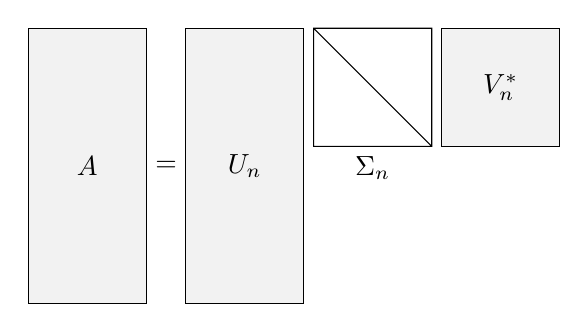
\begin{tikzpicture}[scale=0.5]
  \draw[fill=black!5] (0,0) rectangle node {$A$} +(3,7);
  \node at (3.5,3.5) {=};
  \draw[fill=black!5] (4,0) rectangle node {$U_n$} +(3,7);
  \draw (7.25,4) rectangle +(3,3) (7.25,7) -- +(3,-3);
  \node[below] at (8.75,4) {$\Sigma_n$};
  \draw[fill=black!5] (10.5,4) rectangle node {$V_n^*$} +(3,3);
\end{tikzpicture}
\caption{\label{fig:svd}Scheme of the thin SVD of a rectangular matrix $A$.}
\end{figure}

In the following, we will assume that $m\geq n$. If $m<n$ then $A$ should be replaced by $A^*$ (note that in \slepc this is done transparently as described later in this chapter and the user need not worry about this). In the case that $m\geq n$, the top $n$ rows of $\Sigma$ contain $\mathrm{diag}(\sigma_1,\ldots,\sigma_n)$ and its bottom $m-n$ rows are zero. The relation \eqref{eq:svd} may also be written as $AV=U\Sigma$, or
\begin{equation}
\label{eq:svdleft}
Av_i=u_i\sigma_i\;,\quad i=1,\ldots,n,
\end{equation}
and also as $A^*U=V\Sigma^*$, or
\begin{align}
\label{eq:svdright}
A^*u_i&=v_i\sigma_i\;,\quad i=1,\ldots,n,\\
\label{eq:svdright2}
A^*u_i&=0\;,\quad i=n+1,\ldots,m.
\end{align}
The last left singular vectors corresponding to \eqref{eq:svdright2} are often not computed, especially if $m\gg n$. In that case, the resulting factorization is sometimes called the \emph{thin} SVD, $A=U_n\Sigma_n V_n^*$, and is depicted in Figure \ref{fig:svd}. This factorization can also be written as
\begin{equation}
\label{eq:svdouter}
A=\sum_{i=1}^{n}\sigma_iu_iv_i^*.
\end{equation}
Each $(\sigma_i,u_i,v_i)$ is called a singular triplet.

The singular values are real and nonnegative, $\sigma_1\geq\sigma_2\geq\ldots\geq\sigma_r>\sigma_{r+1}=\ldots=\sigma_n=0$, where $r=\mathrm{rank}(A)$. It can be shown that $\{u_1,\ldots,u_r\}$ span the range of $A$, $\mathcal{R}(A)$, whereas $\{v_{r+1},\ldots,v_n\}$ span the null space of $A$, $\mathcal{N}(A)$.

If the zero singular values are dropped from the sum in \eqref{eq:svdouter}, the resulting factorization, $A=\sum_{i=1}^{r}\sigma_iu_iv_i^*$, is called the \emph{compact} SVD, $A=U_r\Sigma_r V_r^*$.

In the case of a very large and sparse $A$, it is usual to compute only a subset of $k\leq r$ singular triplets. We will refer to this decomposition as the \emph{truncated} SVD of $A$. It can be shown that the matrix $A_k=U_k\Sigma_k V_k^*$ is the best rank-$k$ approximation to matrix $A$, in the least squares sense.

In general, one can take an arbitrary subset of the summands in \eqref{eq:svdouter}, and the resulting factorization is called the \emph{partial} SVD of $A$. As described later in this chapter, \slepc allows the computation of a partial SVD corresponding to either the $k$ largest or smallest singular triplets.

\paragraph{Equivalent Eigenvalue Problems.}

It is possible to formulate the problem of computing the singular triplets of a matrix $A$ as an eigenvalue problem involving a Hermitian matrix related to $A$. There are two possible ways of achieving this:
\begin{enumerate}
\item With the \emph{cross product} matrix, either $A^*A$ or $AA^*$.
\item With the \emph{cyclic} matrix, $H(A)=\left[\begin{smallmatrix}0&A\\A^*&0\end{smallmatrix}\right]$.
\end{enumerate}
In \slepc, the computation of the SVD is usually based on one of these two alternatives, either by passing one of these matrices to an \ident{EPS} object or by performing the computation implicitly.

By pre-multiplying \eqref{eq:svdleft} by $A^*$ and then using \eqref{eq:svdright}, the following relation results
\begin{equation}
\label{eq:eigleft}
A^*Av_i=\sigma_i^2v_i,
\end{equation}
that is, the $v_i$ are the eigenvectors of matrix $A^*A$ with corresponding eigenvalues equal to $\sigma_i^2$. Note that after computing $v_i$ the corresponding left singular vector, $u_i$, is readily available through \eqref{eq:svdleft} with just a matrix-vector product, $u_i=\frac{1}{\sigma_i}Av_i$.

Alternatively, one could first compute the left vectors and then the right ones. For this, pre-multiply \eqref{eq:svdright} by $A$ and then use \eqref{eq:svdleft} to get
\begin{equation}
\label{eq:eigright}
AA^*u_i=\sigma_i^2u_i.
\end{equation}
In this case, the right singular vectors are obtained as $v_i=\frac{1}{\sigma_i}A^*u_i$.

The two approaches represented in \eqref{eq:eigleft} and \eqref{eq:eigright} are very similar. Note however that $A^*A$ is a square matrix of order $n$ whereas $AA^*$ is of order $m$. In cases where $m\gg n$, the computational effort will favor the $A^*A$ approach. On the other hand, the eigenproblem \eqref{eq:eigleft} has $n-r$ zero eigenvalues and the eigenproblem \eqref{eq:eigright} has $m-r$ zero eigenvalues. Therefore, continuing with the assumption that $m\geq n$, even in the full rank case the $AA^*$ approach may have a large null space resulting in difficulties if the smallest singular values are sought. In \slepc, this will be referred to as the cross product approach and will use whichever matrix is smaller, either $A^*A$ or $AA^*$.

Computing the SVD via the cross product approach may be adequate for determining the largest singular triplets of $A$, but the loss of accuracy can be severe for the smallest singular triplets. The cyclic matrix approach is an alternative that avoids this problem, but at the expense of significantly increasing the cost of the computation. Consider the eigendecomposition of
\begin{equation}
\label{eq:cyclic}
H(A)=\begin{bmatrix}0&A\\A^*&0\end{bmatrix},
\end{equation}
which is a Hermitian matrix of order $(m+n)$. It can be shown that $\pm\sigma_i$ is a pair of eigenvalues of $H(A)$ for $i=1,\ldots,r$ and the other $m+n-2r$ eigenvalues are zero. The unit eigenvectors associated with $\pm\sigma_i$ are $\frac{1}{\sqrt{2}}\left[\begin{smallmatrix}\pm u_i\\v_i\end{smallmatrix}\right]$. Thus it is possible to extract the singular values and the left and right singular vectors of $A$ directly from the eigenvalues and eigenvectors of $H(A)$. Note that in this case the singular values are not squared, and therefore the computed values will be more accurate (especially the small ones). The drawback in this case is that small eigenvalues are located in the interior of the spectrum.

\subsection{\label{sec:gsvd}The Generalized Singular Value Decomposition (GSVD)}

An extension of the SVD to the case of two matrices is the generalized singular value decomposition (GSVD), which can be applied in constrained least squares problems, among others. An overview of the problem can be found in~\citep[\S 8.7.3]{Golub:1996:MC}.

Consider two matrices, $A\in\mathbb{C}^{m\times n}$ with $m\geq n$ and $B\in\mathbb{C}^{p\times n}$. Note that both matrices must have the same column dimension. Then there exist two unitary matrices $U\in\mathbb{C}^{m\times m}$ and $V\in\mathbb{C}^{p\times p}$ and an invertible matrix $X\in\mathbb{C}^{n\times n}$ such that
\begin{equation}
\label{eq:gsvd}
U^*AX=C,\qquad V^*BX=S,
\end{equation}
where $C=\mathrm{diag}(c_1,\dots,c_n)$ and $S=\mathrm{diag}(s_{n-q+1},\dots,s_n)$ with $q=\min(p,n)$. The values $c_i$ and $s_i$ are real and nonnegative, and the ratios define the generalized singular values,
\begin{equation}
\label{eq:gsvd-values}
\sigma(A,B)\equiv\{c_1/s_1,\dots,c_q/s_q\},
\end{equation}
and if $p<n$ we can consider that the first $n-p$ generalized singular values are infinite, as if $s_1=\dots=s_{n-p}=0$. Note that if $B$ is the identity matrix, $X$ can be taken to be unitary and then we recover the standard SVD, $\sigma(A,I)=\sigma(A)$, that is why \eqref{eq:gsvd} is considered a generalization of the SVD.

The diagonal matrices $C$ and $S$ satisfy $C^*C+S^*S=I$, and are related to the CS decomposition~\citep[\S 2.6.4]{Golub:1996:MC} associated with the orthogonal factor of the QR factorization of matrices $A$ and $B$ stacked, that is, if
\begin{equation}
\label{eq:cs}
Z:=\begin{bmatrix}A\\B\end{bmatrix}=\begin{bmatrix}Q_1\\Q_2\end{bmatrix}R,
\end{equation}
then $C$ and $S$ can be obtained from the singular values of $Q_1$ and $Q_2$, respectively. The matrix $Z$ is relevant for algorithms and is often built explicitly.

\begin{figure}
\centering
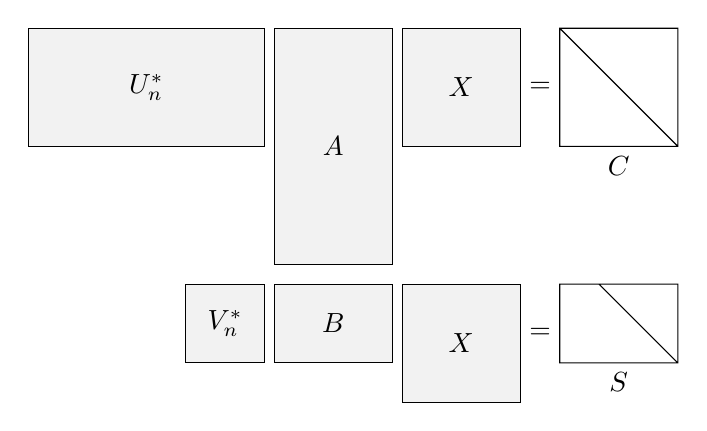
\begin{tikzpicture}[scale=0.5]
  \draw[fill=black!5] (-6.25,3) rectangle node {$U_n^*$} +(6,3);
  \draw[fill=black!5] (0,0) rectangle node {$A$} +(3,6);
  \draw[fill=black!5] (3.25,3) rectangle node {$X$} +(3,3);
  \node at (6.75,4.5) {=};
  \draw (7.25,3) rectangle +(3,3) (7.25,6) -- +(3,-3);
  \node[below] at (8.75,3) {$C$};
  \begin{scope}[yshift=-3.5cm]
  \draw[fill=black!5] (-2.25,1) rectangle node {$V_n^*$} +(2,2);
  \draw[fill=black!5] (0,1) rectangle node {$B$} +(3,2);
  \draw[fill=black!5] (3.25,0) rectangle node {$X$} +(3,3);
  \node at (6.75,1.75) {=};
  \draw (7.25,1) rectangle +(3,2) ++(3,0) -- +(-2,2);
  \node[below] at (8.75,1) {$S$};
  \end{scope}
\end{tikzpicture}
\caption{\label{fig:gsvd}Scheme of the thin GSVD of two matrices $A$ and $B$, for the case $p<n$.}
\end{figure}

The above description assumes that matrix $Z$ has full column rank, and the rank of $B$ is also $q$. In the general case where these assumptions do not hold, the structure of matrices $C$ and $S$ is a bit more complicated. This includes also the case where $m<n$. A detailed description of those cases can be found in~\citep[\S 2.3.5.3]{Anderson:1999:LUG}.

As in the case of the SVD, one can consider thin, compact, truncated, and partial versions of the GSVD. A pictorial representation of the thin GSVD is shown in Figure \ref{fig:gsvd}.

The columns of $X$, $x_i$, are called the (right) generalized singular vectors. The left vectors in this case would correspond to the columns of $U$ and $V$. In SLEPc, the user interface will provide these vectors stacked on top of each other, as a single $(m+p)$-vector $\begin{bmatrix}u_i\\v_i\end{bmatrix}$.

\paragraph{Equivalent Eigenvalue Problems.}
In the GSVD it is also possible to formulate the problem as an eigenvalue problem, which opens the door to approach its solution via \ident{EPS}. The columns of $X$ satisfy
\begin{equation}
\label{eq:gsvdeigcross}
s_i^2A^*Ax_i=c_i^2B^*Bx_i,
\end{equation}
and so if $s_i\neq 0$ then $A^*Ax_i=\sigma_i^2B^*Bx_i$, a generalized eigenvalue problem for the matrix pair $(A^*A,B^*B)$. This is the analog of the cross product matrix eigenproblem of~\eqref{eq:eigleft}.

The formulation that is analog to the eigenproblem associated with the cyclic matrix~\eqref{eq:cyclic} is to solve the generalized eigenvalue problem defined by any of the matrix pairs
\begin{equation}
\label{eq:gsvdeigcyclic}
\left(
\begin{bmatrix}0&A\\A^*&0\end{bmatrix},
\begin{bmatrix}I&0\\0&B^*B\end{bmatrix}
\right),
\qquad\text{or}\qquad
\left(
\begin{bmatrix}0&B\\B^*&0\end{bmatrix},
\begin{bmatrix}I&0\\0&A^*A\end{bmatrix}
\right).
\end{equation}

%---------------------------------------------------
\section{Basic Usage}

From the perspective of the user interface, the \ident{SVD} package is very similar to \ident{EPS}, with some differences that will be highlighted shortly.

\begin{figure}
\begin{Verbatim}[fontsize=\small,numbers=left,numbersep=6pt,xleftmargin=15mm]
SVD       svd;       /*  SVD solver context  */
Mat       A;         /*  problem matrix      */
Vec       u, v;      /*  singular vectors    */
PetscReal sigma;     /*  singular value      */
PetscInt  j, nconv;
PetscReal error;

SVDCreate( PETSC_COMM_WORLD, &svd );
SVDSetOperators( svd, A, NULL );
SVDSetProblemType( svd, SVD_STANDARD );
SVDSetFromOptions( svd );
SVDSolve( svd );
SVDGetConverged( svd, &nconv );
for (j=0; j<nconv; j++) {
  SVDGetSingularTriplet( svd, j, &sigma, u, v );
  SVDComputeError( svd, j, SVD_ERROR_RELATIVE, &error );
}
SVDDestroy( &svd );
\end{Verbatim}
\caption{\label{fig:ex-svd}Example code for basic solution with \ident{SVD}.}
\end{figure}

The basic steps for computing a partial SVD with \slepc are illustrated in Figure \ref{fig:ex-svd}. The steps are more or less the same as those described in chapter \ref{cap:eps} for the eigenvalue problem. First, the solver context is created with \ident{SVDCreate}. Then the problem matrices have to be specified with \ident{SVDSetOperators} and the type of problem can be selected via \ident{SVDSetProblemType}. Then, a call to \ident{SVDSolve} invokes the actual solver. After that, \ident{SVDGetConverged} is used to determine how many solutions have been computed, which are retrieved with \ident{SVDGetSingularTriplet}. Finally, \ident{SVDDestroy} gets rid of the object.

If one compares this example code with the \ident{EPS} example in Figure \ref{fig:ex-eps}, the most outstanding differences are the following:
\begin{itemize}
\item The singular value is a \texttt{PetscReal}, not a \texttt{PetscScalar}.
\item Each singular vector is defined with a single \texttt{Vec} object, not two as was the case for eigenvectors.
\end{itemize}

%---------------------------------------------------
\section{Defining the Problem}

Defining the problem consists in specifying the problem matrix $A$ (and also a second matrix $B$ in case of the GSVD), the problem type, and the portion of the spectrum to be computed.

The problem matrices are provided with the following function
	\findex{SVDSetOperators}
	\begin{Verbatim}[fontsize=\small]
	SVDSetOperators(SVD svd,Mat A,Mat B);
	\end{Verbatim}
where \texttt{A} can be any matrix, not necessarily square, stored in any allowed \petsc format including the matrix-free mechanism (see \S\ref{sec:supported} for a detailed discussion), and \texttt{B} is generally set to \texttt{NULL} except in the case of computing the GSVD.

The problem type can be specified with the function
	\findex{SVDSetProblemType}
	\begin{Verbatim}[fontsize=\small]
	SVDSetProblemType(SVD svd,SVDProblemType type);
	\end{Verbatim}
Note that in \ident{SVD} calling it is currently not strictly required, since if only one matrix is passed to \ident{SVDSetOperators} the problem type will default to a standard SVD, while if two matrices are passed then it defaults to GSVD. Table~\ref{tab:ptypesvd} lists the supported problem types.

\begin{table}[t]
\centering
{\small \begin{tabular}{lll}
Problem Type              & \ident{SVDProblemType}    & Command line key\\\hline
Standard SVD              & \texttt{SVD\_STANDARD}    & \texttt{-svd\_standard}\\
Generalized SVD (GSVD)    & \texttt{SVD\_GENERALIZED} & \texttt{-svd\_generalized}\\\hline
\end{tabular} }
\caption{\label{tab:ptypesvd}Problem types considered in \ident{SVD}.}
\end{table}

It is important to note that all SVD solvers in \slepc make use of both $A$ and $A^*$, as suggested by the description in \S\ref{sec:svd}. $A^*$ is not explicitly passed as an argument to \ident{SVDSetOperators}, therefore it will have to stem from $A$. There are two possibilities for this: either $A$ is transposed explicitly and $A^*$ is created as a distinct matrix, or $A^*$ is handled implicitly via \ident{MatMultTranspose} (or \ident{MatMultHermitianTranspose} in the complex case) operations whenever a matrix-vector product is required in the algorithm. The default is to build $A^*$ explicitly, but this behavior can be changed with
	\findex{SVDSetImplicitTranspose}
	\begin{Verbatim}[fontsize=\small]
	SVDSetImplicitTranspose(SVD svd,PetscBool impl);
	\end{Verbatim}

In \S\ref{sec:svd}, it was mentioned that in \slepc the cross product approach chooses the smallest of the two possible cases $A^*A$ or $AA^*$, that is, $A^*A$ is used if $A$ is a tall, thin matrix ($m\geq n$), and $AA^*$ is used if $A$ is a fat, short matrix ($m<n$). In fact, what \slepc does internally is that if $m<n$ the roles of $A$ and $A^*$ are reversed. This is equivalent to transposing all the SVD factorization, so left singular vectors become right singular vectors and vice versa. This is actually done in all singular value solvers, not only the cross product approach. The objective is to simplify the number of cases to be treated internally by \slepc, as well as to reduce the computational cost in some situations. Note that this is done transparently and the user need not worry about transposing the matrix, only to indicate how the transpose has to be handled, as explained above.

The user can specify how many singular values and vectors to compute. The default is to compute only one singular triplet. The function
	\findex{SVDSetDimensions}
	\begin{Verbatim}[fontsize=\small]
	SVDSetDimensions(SVD svd,PetscInt nsv,PetscInt ncv,PetscInt mpd);
	\end{Verbatim}
allows the specification of the number of singular values to compute, \texttt{nsv}. The next argument can be set to prescribe the number of column vectors to be used by the solution algorithm, \texttt{ncv}, that is, the largest dimension of the working subspace. These two parameters can also be set at run time with the options \Verb!-svd_nsv! and \Verb!-svd_ncv!. For example, the command line
\begin{Verbatim}[fontsize=\small]
	$ ./program -svd_nsv 10 -svd_ncv 24
\end{Verbatim}
requests 10 singular values and instructs to use 24 column vectors. Note that \texttt{ncv} must be at least equal to \texttt{nsv}, although in general it is recommended (depending on the method) to work with a larger subspace, for instance $\mathtt{ncv}\geq2\cdot\mathtt{nsv}$ or even more.
As in the case of the \ident{EPS} object, the last argument, \texttt{mpd}, can be used to limit the maximum dimension of the projected problem, as discussed in \S\ref{sec:large-nev}. Using this parameter is especially important in the case that a large number of singular values are requested.

\begin{table}
\centering
{\small \begin{tabular}{lll}
\texttt{SVDWhich}                  & Command line key                   & Sorting criterion \\\hline
\texttt{SVD\_LARGEST}   & \texttt{-svd\_largest}  & Largest $\sigma$ \\
\texttt{SVD\_SMALLEST}  & \texttt{-svd\_smallest} & Smallest $\sigma$ \\\hline
\end{tabular} }
\caption{\label{tab:whichsvd}Available possibilities for selection of the singular values of interest.}
\end{table}

	For the selection of the portion of the spectrum of interest, there are only two possibilities in the case of SVD: largest and smallest singular values, see Table \ref{tab:whichsvd}. The default is to compute the largest ones, but this can be changed with
	\findex{SVDSetWhichSingularTriplets}
	\begin{Verbatim}[fontsize=\small]
	SVDSetWhichSingularTriplets(SVD svd,SVDWhich which);
	\end{Verbatim}
which can also be specified at the command line. This criterion is used both for configuring how the algorithm seeks singular values and also for sorting the computed values. In contrast to the case of \ident{EPS}, computing singular values located in the interior part of the spectrum is difficult, the only possibility is to use an \ident{EPS} object combined with a spectral transformation (this possibility is explained in detail in the next section). Note that in this case, the value of \Verb!which! applies to the transformed spectrum.

%---------------------------------------------------
\section{Selecting the SVD Solver}

The available methods for computing the partial SVD are shown in Table \ref{tab:svdsolvers}. These methods can be classified in the following three groups:
\begin{itemize}
\item Solvers based on \ident{EPS}. These solvers set up an \ident{EPS} object internally, thus using the available eigensolvers for solving the SVD problem. The two possible approaches in this case are the cross product matrix and the cyclic matrix, as described in \S\ref{sec:svd}.
\item Specific SVD solvers. These are typically eigensolvers that have been adapted algorithmically to exploit the structure of the SVD problem. There are currently two solvers in this category: Lanczos and thick-restart Lanczos. A detailed description of these methods can be found in \hyperlink{str}{[STR-8]}.
\item The \lapack solver. This is an interface to some LAPACK routines, analog of those in the case of eigenproblems. These routines operate in dense mode with only one processor and therefore are suitable only for moderate size problems. This solver should be used only for debugging purposes.
\item External packages: \scalapack and \elemental are dense packages and compute the complete SVD, while \primme offers Davidson-type methods to compute only a few singular triplets.
\end{itemize}
The default solver is the one that uses the cross product matrix (\texttt{cross}), usually the fastest and most memory-efficient approach. See a more detailed explanation below.

\begin{table}
\centering
{\small \begin{tabular}{lllll}
                           &                        & {\footnotesize Options} & Supports & \\
Method                     & \ident{SVDType}        & {\footnotesize Database Name}& GSVD &Default \\\hline
Cross Product              & \texttt{SVDCROSS}      & \texttt{cross}        & yes & $\star$ \\
Cyclic Matrix              & \texttt{SVDCYCLIC}     & \texttt{cyclic}       & yes & \\
Lanczos                    & \texttt{SVDLANCZOS}    & \texttt{lanczos}      & & \\
Thick-restart Lanczos      & \texttt{SVDTRLANCZOS}  & \texttt{trlanczos}    & yes & \\
Randomized SVD (RSVD)      & \texttt{SVDRANDOMIZED} & \texttt{randomized}   & & \\\hline
\lapack solver             & \texttt{SVDLAPACK}     & \texttt{lapack}       & yes & \\
Wrapper to \scalapack      & \texttt{SVDSCALAPACK}  & \texttt{scalapack}    & & \\
Wrapper to \elemental      & \texttt{SVDELEMENTAL}  & \texttt{elemental}    & & \\
Wrapper to \primme         & \texttt{SVDPRIMME}     & \texttt{primme}       & & \\\hline
\end{tabular} }
\caption{\label{tab:svdsolvers}List of solvers available in the \ident{SVD} module.}
\end{table}

The solution method can be specified procedurally or via the command line. The application programmer can set it by means of the command
	\findex{SVDSetType}
	\begin{Verbatim}[fontsize=\small]
	SVDSetType(SVD svd,SVDType method);
	\end{Verbatim}
while the user writes the options database command \Verb!-svd_type! followed by the name of the method (see Table \ref{tab:svdsolvers}).

Note that not all solvers in the \ident{SVD} module support the GSVD problem of \S\ref{sec:gsvd}. Table \ref{tab:svdsolvers} indicates which solvers can be used for this.

The \ident{EPS}-based solvers deserve some additional comments. These SVD solvers work by creating an \ident{EPS} object internally and setting up an eigenproblem of type \ident{EPS\_HEP}. These solvers implement the cross product matrix approach \eqref{eq:eigleft}, and the cyclic matrix approach \eqref{eq:cyclic}. Therefore, the operator matrix associated with the \ident{EPS} object will be $A^*A$ in the case of the \texttt{cross} solver and $H(A)$ in the case of the \texttt{cyclic} solver.

In the case of the \texttt{cross} solver, the matrix $A^*A$ is not built explicitly by default, since the resulting matrix may be much less sparse than the original matrix. By default, a shell matrix is created internally in the \ident{SVD} object and passed to the \ident{EPS} object. Still, the user may choose to force the computation of $A^*A$ explicitly, by means of \petsc's sparse matrix-matrix product subroutines. This is set with
	\findex{SVDCrossSetExplicitMatrix}
	\begin{Verbatim}[fontsize=\small]
	SVDCrossSetExplicitMatrix(SVD svd,PetscBool explicit);
	\end{Verbatim}
In the \texttt{cyclic} solver the user can also choose between handling $H(A)$ implicitly as a shell matrix (the default), or forming it explicitly, that is, storing its elements in a distinct matrix. The function for setting this option is
	\findex{SVDCyclicSetExplicitMatrix}
	\begin{Verbatim}[fontsize=\small]
	SVDCyclicSetExplicitMatrix(SVD svd,PetscBool explicit);
	\end{Verbatim}

The \ident{EPS} object associated with the \texttt{cross} and \texttt{cyclic} SVD solvers is created with a set of reasonable default parameters. However, it may sometimes be necessary to change some of the \ident{EPS} options such as the eigensolver. To allow application programmers to set any of the \ident{EPS} options directly within the code, the following routines are provided to extract the \ident{EPS} context from the \ident{SVD} object,
	\findex{SVDCrossGetEPS}
	\findex{SVDCyclicGetEPS}
	\begin{Verbatim}[fontsize=\small]
	SVDCrossGetEPS(SVD svd,EPS *eps);
	SVDCyclicGetEPS(SVD svd,EPS *eps);
	\end{Verbatim}
A more convenient way of changing \ident{EPS} options is through the command-line. This is achieved simply by prefixing the \ident{EPS} options with \texttt{-svd\_cross\_} or \texttt{-svd\_cyclic\_} as in the following example:
\begin{Verbatim}[fontsize=\small]
	$ ./program -svd_type cross -svd_cross_eps_type gd
\end{Verbatim}

At this point, one may consider changing also the options of the \ident{ST} object associated with the \ident{EPS} object in \texttt{cross} and \texttt{cyclic} SVD solvers, for example to compute singular values located at the interior of the spectrum via a shift-and-invert transformation. This is indeed possible, but some considerations have to be taken into account. When $A^*A$ or $H(A)$ are managed as shell matrices, then the potential of the spectral transformation is limited seriously, because some of the required operations will not be defined if working with implicit matrices (this is discussed briefly in \S\ref{sec:supported} and \S\ref{sec:explicit}). The following example illustrates the computation of interior singular values with the \texttt{cyclic} solver with explicit $H(A)$ matrix:
\begin{Verbatim}[fontsize=\small]
	$ ./program -svd_type cyclic -svd_cyclic_explicitmatrix
                    -svd_cyclic_st_type sinvert -svd_cyclic_eps_target 12.0
                    -svd_cyclic_st_ksp_type preonly -svd_cyclic_st_pc_type lu
\end{Verbatim}

%---------------------------------------------------
\section{Retrieving the Solution}

Once the call to \ident{SVDSolve} is complete, all the data associated with the computed partial SVD is kept internally in the \ident{SVD} object. This information can be obtained by the calling program by means of a set of functions described below.

As in the case of eigenproblems, the number of computed singular triplets depends on the convergence and, therefore, it may be different from the number of solutions requested by the user. So the first task is to find out how many solutions are available, with
	\findex{SVDGetConverged}
	\begin{Verbatim}[fontsize=\small]
	SVDGetConverged(SVD svd,PetscInt *nconv);
	\end{Verbatim}
Usually, the number of converged solutions, \texttt{nconv}, will be equal to \texttt{nsv}, but in general it can be a number ranging from 0 to \texttt{ncv} (here, \texttt{nsv} and \texttt{ncv} are the arguments of function \ident{SVDSetDimensions}).

Normally, the user is interested in the singular values only, or the complete singular triplets. The function
	\findex{SVDGetSingularTriplet}
	\begin{Verbatim}[fontsize=\small]
	SVDGetSingularTriplet(SVD svd,PetscInt j,PetscReal *sigma,Vec u,Vec v);
	\end{Verbatim}
returns the $j$-th computed singular triplet, $(\sigma_j,u_j,v_j)$, where both $u_j$ and $v_j$ are normalized to have unit norm. Typically, this function is called inside a loop for each value of \texttt{j} from 0 to \texttt{nconv}--1. Note that singular values are ordered according to the same criterion specified with function \ident{SVDSetWhichSingularTriplets} for selecting the portion of the spectrum of interest.

In some applications, it may be enough to compute only the right singular vectors. This is especially important in cases in which memory requirements are critical (remember that both $U_k$ and $V_k$ are dense matrices, and $U_k$ may require much more storage than $V_k$, see Figure \ref{fig:svd}). In \slepc, there is no general option for specifying this, but the default behavior of some solvers is to compute only right vectors and allocate/compute left vectors only in the case that the user requests them. This is done in the \texttt{cross} solver and in some special variants of other solvers such as one-sided Lanczos (consult the \hyperlink{str}{[STR-8]} technical report for specific solver options).

In the case of the GSVD, the \texttt{sigma} argument of \ident{SVDGetSingularTriplet} contains $\sigma_i=c_i/s_i$ and the second \texttt{Vec} argument (\texttt{v}) contains the right singular vectors ($x_i$), while the first \texttt{Vec} argument (\texttt{u}) contains the other vectors of the decomposition stacked on top of each other, as a single $(m+p)$-vector: $\begin{bmatrix}u_i\\v_i\end{bmatrix}$.

\paragraph{Reliability of the Computed Solution.}

In SVD computations, a-posteriori error bounds are much the same as in the case of Hermitian eigenproblems, due to the equivalence discussed in \S\ref{sec:svd}. The residual vector is defined in terms of the cyclic matrix, $H(A)$, so its norm is
\begin{equation}
\|r_\mathrm{SVD}\|_2=\left(\|A\tilde{v}-\tilde{\sigma}\tilde{u}\|_2^2+\|A^*\tilde{u}-\tilde{\sigma}\tilde{v}\|_2^2\right)^{\frac{1}{2}},
\end{equation}
where $\tilde{\sigma}$, $\tilde{u}$ and $\tilde{v}$ represent any of the \texttt{nconv} computed singular triplets delivered by \texttt{SVDGetSingularTriplet}.

Given the above definition, the following relation holds
\begin{equation}
|\sigma-\tilde{\sigma}|\leq \|r\|_2,
\end{equation}
where $\sigma$ is an exact singular value. The associated error can be obtained in terms of $\|r\|_2$ with the following function:
	\findex{SVDComputeError}
	\begin{Verbatim}[fontsize=\small]
	SVDComputeError(SVD svd,PetscInt j,SVDErrorType type,PetscReal *error);
	\end{Verbatim}

In the case of the GSVD, the function \ident{SVDComputeError} will compute a residual norm based on the two relations~\eqref{eq:gsvd},
\begin{equation}
\|r_\mathrm{GSVD}\|_2=\left(\|\tilde{s}^2A^*\tilde{u}-\tilde{c}B^*B\tilde{x}\|_2^2+\|\tilde{c}^2B^*\tilde{v}-\tilde{s}A^*A\tilde{x}\|_2^2\right)^{\frac{1}{2}},
\end{equation}
where $\tilde{x}$, $\tilde{u}$, $\tilde{v}$ are the computed singular vectors corresponding to $\tilde{\sigma}$, and $\tilde{c}$, $\tilde{s}$ are obtained from $\tilde{\sigma}$ as $\tilde{s}=1/\sqrt{1+\tilde{\sigma}^2}$ and $\tilde{c}=\tilde{\sigma}\tilde{s}$. See~\citep{Alvarruiz:2022:TRL} for details.

\paragraph{Controlling and Monitoring Convergence.}

Similarly to the case of eigensolvers, in \ident{SVD} the number of iterations carried out by the solver can be determined with \ident{SVDGetIterationNumber}, and the tolerance and maximum number of iterations can be set with \ident{SVDSetTolerances}. Also, convergence can be monitored with command-line keys \Verb!-svd_monitor!, \Verb!-svd_monitor_all!, \Verb!-svd_monitor_conv!, or graphically with \Verb!-svd_monitor draw::draw_lg!, or alternatively with \Verb!-svd_monitor_all draw::draw_lg!. See \S\ref{sec:monitor} for additional details.

\begin{table}
\centering
{\small \begin{tabular}{llll}
Convergence criterion      & \texttt{SVDConv}          & Command line key           & Error bound \\\hline
Absolute                   & \texttt{SVD\_CONV\_ABS}   & \texttt{-svd\_conv\_abs}   & $\|r\|$ \\
Relative to eigenvalue     & \texttt{SVD\_CONV\_REL}   & \texttt{-svd\_conv\_rel}   & $\|r\|/|\lambda|$ \\
Relative to matrix norms   & \texttt{SVD\_CONV\_NORM}  & \texttt{-svd\_conv\_norm}  & $\|r\|/\|A\|$ \\
Fixed number of iterations & \texttt{SVD\_CONV\_MAXIT} & \texttt{-svd\_conv\_maxit} & $\infty$ \\
User-defined               & \texttt{SVD\_CONV\_USER}  & \texttt{-svd\_conv\_user}  & user function \\
\hline
\end{tabular} }
\caption{\label{tab:svdconvergence}Available possibilities for the convergence criterion.}
\end{table}

As in the case of eigensolvers, the user can choose different convergence tests, based on an error bound obtained from the computed residual norm, $\|r\|$. Table \ref{tab:svdconvergence} lists the available options. It is worth mentioning the \texttt{SVD\_CONV\_MAXIT} convergence criterion, which is a bit special. With this criterion, the solver will not compute any residual norms and will stop with a successful status when the maximum number of iterations is reached. This is intended for the \texttt{SVDRANDOMIZED} solver in cases when a low-rank approximation of a matrix needs to be computed instead of accurate singular vectors.

\paragraph{Viewing the Solution.}

There is support for different kinds of viewers for the solution, as in the case of eigensolvers. One can for instance use \Verb!-svd_view_values!, \Verb!-svd_view_vectors!, \Verb!-svd_error_relative!, or \Verb!-svd_converged_reason!. See description in \S\ref{sec:epsviewers}.


%-------------------------------------------------------
% SLEPc Users Manual
%-------------------------------------------------------
\chapter{\label{cap:pep}PEP: Polynomial Eigenvalue Problems}
%-------------------------------------------------------

\begin{center}
  {\setlength{\fboxsep}{4mm}
  \framebox{%
   \begin{minipage}{.8\textwidth}
   \textbf{Note:} Previous \slepc versions provided specific functionality for quadratic eigenvalue problems (the \texttt{QEP} module). This has been made more general by covering polynomials of arbitrary degree (the \texttt{PEP} module described in this chapter), which of course includes quadratic problems as a particular case. See \S\ref{sec:qeppep} for how to upgrade application code that used \texttt{QEP}.
   \end{minipage}
  }}
\end{center}

\noindent The Polynomial Eigenvalue Problem (\ident{PEP}) solver object is intended for addressing polynomial eigenproblems of arbitrary degree, $P(\lambda)x=0$. A particular instance is the quadratic eigenvalue problem (degree 2), which is the case more often encountered in practice. For this reason, part of the description of this chapter focuses specifically on quadratic eigenproblems.

Currently, all \ident{PEP} solvers are based on linearization, either implicit or explicit. The case of explicit linearization allows the use of eigensolvers from \ident{EPS} to solve the linearized problem.

\section{\label{sec:pep}Overview of Polynomial Eigenproblems}

In this section, we review some basic properties of the polynomial eigenvalue problem. The main goal is to set up the notation as well as to describe the linearization approaches that will be employed for solving via an \ident{EPS} object.
To simplify the description, we initially restrict to the case of quadratic eigenproblems, and then extend to the general case of arbitrary degree.
For additional background material, the reader is referred to \citep{Tisseur:2001:QEP}. As always, some details of the implemented methods can be found in the \slepc \hyperlink{str}{technical reports}.

\subsection{\label{sec:qep}Quadratic Eigenvalue Problems}

In many applications, e.g., problems arising from second-order differential equations such as the analysis of damped vibrating systems, the eigenproblem to be solved is quadratic,
\begin{equation}
(K+\lambda C+\lambda^2M)x=0,\label{eq:eigquad}
\end{equation}
where $K,C,M\in\mathbb{C}^{n\times n}$ are the coefficients of a matrix polynomial of degree 2, $\lambda\in\mathbb{C}$ is the eigenvalue and $x\in\mathbb{C}^n$ is the eigenvector. As in the case of linear eigenproblems, the eigenvalues and eigenvectors can be complex even in the case that all three matrices are real.

It is important to point out some outstanding differences with respect to the linear eigenproblem. In the quadratic eigenproblem, the number of eigenvalues is $2n$, and the corresponding eigenvectors do not form a linearly independent set. If $M$ is singular, some eigenvalues are infinite. Even when the three matrices are symmetric and positive definite, there is no guarantee that the eigenvalues are real, but still methods can exploit symmetry to some extent. Furthermore, numerical difficulties are more likely than in the linear case, so the computed solution can sometimes be untrustworthy.

If Eq.\ \ref{eq:eigquad} is written as $P(\lambda)x=0$, where $P$ is the matrix polynomial, then multiplication by $\lambda^{-2}$ results in $R(\lambda^{-1})x=0$, where $R$ is a matrix polynomial with the coefficients in the reverse order. In other words, if a method is available for computing the largest eigenvalues, then reversing the roles of $M$ and $K$ results in the computation of the smallest eigenvalues. In general, it is also possible to formulate different spectral transformations for computing eigenvalues closest to a given target.

\paragraph{Problem Types.}

As in the case of linear eigenproblems, there are some particular properties of the coefficient matrices that confer a certain structure to the quadratic eigenproblem, e.g., symmetry of the spectrum with respect to the real or imaginary axes. These structures are important as long as the solvers are able to exploit them.

\begin{itemize}
\item Hermitian (symmetric) problems, when $M$, $C$, $K$ are all Hermitian (symmetric). Eigenvalues are real or come in complex conjugate pairs. Furthermore, if $M>0$ and $C,K\geq 0$ then the system is stable, i.e., $\text{Re}(\lambda)\leq 0$.
\item Hyperbolic problems, a particular class of Hermitian problems where $M>0$ and $(x^*Cx)^2>4(x^*Mx)(x^*Kx)$ for all nonzero $x\in\mathbb{C}^n$. All eigenvalues are real, and form two separate groups of $n$ eigenvalues, each of them having linearly independent eigenvectors.
\item Overdamped problems, a specialized type of hyperbolic problems, where $C>0$ and $K\geq 0$. The eigenvalues are non-positive.
\item Gyroscopic problems, when $M$, $K$ are Hermitian, $M>0$, and $C$ is skew-Hermitian, $C=-C^*$. The spectrum is symmetric with respect to the imaginary axis, and in the real case, it has a Hamiltonian structure, i.e., eigenvalues come in quadruples $(\lambda,\bar{\lambda},-\lambda,-\bar{\lambda})$.
\end{itemize}

Currently, the problem type is not exploited by \ident{PEP} solvers, but this may change in the future.

\paragraph{Linearization.}

It is possible to transform the quadratic eigenvalue problem to a linear generalized eigenproblem $L_0y=\lambda L_1y$ by doubling the order of the system, i.e., $L_0,L_1\in\mathbb{C}^{2n\times 2n}$. There are many ways of doing this. 
Below, we show some of the most common linearizations,
which are based on defining the eigenvector of the linear problem as 
\begin{equation}
\label{eq:linevec}
y=\left[\begin{array}{c}x\\x\lambda\end{array}\right].
\end{equation}

\begin{itemize}
\item Non-symmetric linearizations. The resulting matrix pencil has no particular structure.
\begin{equation}
\label{eq:n1}
\mbox{N1:}\qquad
\left[\begin{array}{cc}0 & I\\-K & -C\end{array}\right]-\lambda\left[\begin{array}{cc}I & 0\\0 & M\end{array}\right]
\end{equation}
\begin{equation}
\label{eq:n2}
\mbox{N2:}\qquad
\left[\begin{array}{cc}-K & 0\\0 & I\end{array}\right]-\lambda\left[\begin{array}{cc}C & M\\I & 0\end{array}\right]
\end{equation}

\medskip
\item Symmetric linearizations. If $M$, $C$, and $K$ are all symmetric (Hermitian), the resulting matrix pencil is symmetric (Hermitian), although indefinite.
\begin{equation}
\label{eq:s1}
\mbox{S1:}\qquad
\left[\begin{array}{cc}0 & -K\\-K & -C\end{array}\right]-\lambda\left[\begin{array}{cc}-K & 0\\0 & M\end{array}\right]
\end{equation}
\begin{equation}
\label{eq:s2}
\mbox{S2:}\qquad
\left[\begin{array}{cc}-K & 0\\0 & M\end{array}\right]-\lambda\left[\begin{array}{cc}C & M\\ M & 0\end{array}\right]
\end{equation}

\medskip
\item Hamiltonian linearizations. If the quadratic eigenproblem is gyroscopic, one of the matrices is Hamiltonian and the other is skew-Hamiltonian. The first form (H1) is recommended when $M$ is singular, whereas the second form (H2) is recommended when $K$ is singular.
\begin{equation}
\label{eq:h1}
\mbox{H1:}\qquad
\left[\begin{array}{cc}K & 0\\C & K\end{array}\right]-\lambda\left[\begin{array}{cc} 0 & K\\-M & 0\end{array}\right]
\end{equation}
\begin{equation}
\label{eq:h2}
\mbox{H2:}\qquad
\left[\begin{array}{cc}0 & -K\\M & 0\end{array}\right]-\lambda\left[\begin{array}{cc}M & C\\ 0 & M\end{array}\right]
\end{equation}
\end{itemize}

In \slepc, the \ident{PEPLINEAR} solver is based on using one of the above linearizations for solving the quadratic eigenproblem. This solver makes use of linear eigensolvers from the \ident{EPS} package.

We could also consider the \emph{reversed} forms, e.g., the reversed form of N2 is
\begin{equation}
\label{eq:n2r}
\mbox{N2-R:}\qquad
\left[\begin{array}{cc}-C & -M\\I & 0\end{array}\right]-\frac{1}{\lambda}\left[\begin{array}{cc}K & 0\\0 & I\end{array}\right],
\end{equation}
which is equivalent to the form N1 for the problem $R(\lambda^{-1})x=0$. These reversed forms are not implemented in \slepc, but the user can use them simply by reversing the roles of $M$ and $K$, and considering the reciprocals of the computed eigenvalues. Alternatively, this is can be viewed as a particular case of the spectral transformation (with $\sigma=0$), see \S\ref{sec:qst}.

\subsection{\label{sec:pep1}Polynomials of Arbitrary Degree}

In general, the polynomial eigenvalue problem can be formulated as
\begin{equation}
\label{eq:pep}
P(\lambda)x=0,
\end{equation}
where $P$ is an $n\times n$ matrix polynomial of degree $d$. An $n$-vector $x\neq 0$ satisfying this equation is called an eigenvector associated with the corresponding eigenvalue $\lambda$.

We start by considering the case where $P$ is expressed in terms of the monomial basis,
\begin{equation}
\label{eq:pepmon}
P(\lambda)=A_0+A_1 \lambda+A_2\lambda^2 +  \dotsb + A_d \lambda^d,
\end{equation}
where $A_0,\ldots,A_d$ are the $n\times n$ coefficient matrices. As before, the problem can be solved via some kind of linearization. One of the most commonly used one is the first companion form 
\begin{equation}
\label{eq:firstcomp}
L(\lambda)=L_0 -\lambda L_1,
\end{equation}
where the related linear eigenproblem is $L(\lambda)y=0$, with
\begin{equation}
\label{eq:firstcompfull}
	L_0 =
	\begin{bmatrix}
		  & I \\
		 &   & \ddots \\
		 & &    & I \\
		-A_0 & -A_1 & \cdots  & -A_{d-1}
	\end{bmatrix},
	\quad
	L_1 =
	\begin{bmatrix}
		I \\
		 & \ddots \\
		 & & I \\
		 & & & A_d
	\end{bmatrix},
        \quad y=
	\begin{bmatrix}
        x \\ x\lambda\\ \vdots \\ x\lambda^{d-1}
	\end{bmatrix}.
\end{equation}
This is the generalization of Eq.\ \ref{eq:n1}.

The definition of vector $y$ above contains the successive powers of $\lambda$. For large polynomial degree, these values may produce overflow in finite precision computations, or at least lead to numerical instability of the algorithms due to the wide difference in magnitude of the eigenvector entries. For this reason, it is generally recommended to work with non-monomial polynomial bases whenever the degree is not small, e.g., for $d>5$.

In the most general formulation of the polynomial eigenvalue problem, $P$ is expressed as
\begin{equation}
\label{eq:pepnonmon}
P(\lambda)=A_0\phi_0(\lambda)+A_1\phi_1(\lambda)+\dots+A_d\phi_d(\lambda),
\end{equation}
where $\phi_i$ are the members of a given polynomial basis, for instance, some kind of orthogonal polynomials such as Chebyshev polynomials of the first kind. In that case, the expression of $y$ in Eq.\ \ref{eq:firstcompfull} contains $\phi_0(\lambda),\dots,\phi_d(\lambda)$ instead of the powers of $\lambda$. Correspondingly, the form of $L_0$ and $L_1$ is different for each type of polynomial basis.

%---------------------------------------------------
\section{Basic Usage}

The user interface of the \ident{PEP} package is very similar to \ident{EPS}. For basic usage, the most noteworthy difference is that all coefficient matrices $A_i$ have to be supplied in the form of an array of \ident{Mat}.

A basic example code for solving a polynomial eigenproblem with \ident{PEP} is shown in Figure \ref{fig:ex-pep}, where the code for building matrices \texttt{A[0]}, \texttt{A[1]}, \ldots\ is omitted. The required steps are the same as those described in chapter \ref{cap:eps} for the linear eigenproblem. As always, the solver context is created with \ident{PEPCreate}. The coefficient matrices are provided with \ident{PEPSetOperators}, and the problem type is specified with \ident{PEPSetProblemType}. Calling \ident{PEPSetFromOptions} allows the user to set up various options through the command line. The call to \ident{PEPSolve} invokes the actual solver. Then, the solution is retrieved with \ident{PEPGetConverged} and \ident{PEPGetEigenpair}. Finally, \ident{PEPDestroy} destroys the object.

\begin{figure}
\begin{Verbatim}[fontsize=\small,numbers=left,numbersep=6pt,xleftmargin=15mm]
#define NMAT 5

PEP         pep;       /*  eigensolver context  */
Mat         A[NMAT];   /*  coefficient matrices */
Vec         xr, xi;    /*  eigenvector, x       */
PetscScalar kr, ki;    /*  eigenvalue, k        */
PetscInt    j, nconv;
PetscReal   error;

PEPCreate( PETSC_COMM_WORLD, &pep );
PEPSetOperators( pep, NMAT, A );
PEPSetProblemType( pep, PEP_GENERAL );  /* optional */
PEPSetFromOptions( pep );
PEPSolve( pep );
PEPGetConverged( pep, &nconv );
for (j=0; j<nconv; j++) {
  PEPGetEigenpair( pep, j, &kr, &ki, xr, xi );
  PEPComputeRelativeError( pep, j, &error );
}
PEPDestroy( &pep );
\end{Verbatim}
\caption{\label{fig:ex-pep}Example code for basic solution with \ident{PEP}.}
\end{figure}


%---------------------------------------------------
\section{Defining the Problem}

\begin{table}[t]
\centering
{\small \begin{tabular}{lll}
                   &                      & {\footnotesize Options} \\
Polynomial Basis     & \ident{PEPBasis}                & {\footnotesize Database Name}\\\hline
Monomial             & \texttt{PEP\_BASIS\_MONOMIAL}   & \texttt{monomial}\\
Chebyshev (1st kind) & \texttt{PEP\_BASIS\_CHEBYSHEV1} & \texttt{chebyshev1}\\
Chebyshev (2nd kind) & \texttt{PEP\_BASIS\_CHEBYSHEV2} & \texttt{chebyshev2}\\
Legendre             & \texttt{PEP\_BASIS\_LEGENDRE}   & \texttt{legendre}\\
Laguerre             & \texttt{PEP\_BASIS\_LAGUERRE}   & \texttt{laguerre}\\
Hermite              & \texttt{PEP\_BASIS\_HERMITE}    & \texttt{hermite}\\\hline
\end{tabular} }
\caption{\label{tab:pepbasis}Polynomial bases available to represent the matrix polynomial in \ident{PEP}.}
\end{table}

As explained in \S\ref{sec:pep1}, the matrix polynomial $P(\lambda)$ can be expressed in term of the monomials $1$, $\lambda$, $\lambda^2,\ldots$, or in a non-monomial basis as in Eq.\ \ref{eq:pepnonmon}. Hence, when defining the problem we must indicate which is the polynomial basis to be used (note that the coefficient matrices $A_i$ are different for different basis representations). By default, a monomial basis is used. Other possible bases are listed in Table \ref{tab:pepbasis}, and can be set with
	\findex{PEPSetBasis}
	\begin{Verbatim}[fontsize=\small]
	PEPSetBasis(PEP pep,PEPBasis basis);
	\end{Verbatim}
or with the command-line key \Verb!-pep_basis <name>!.

\begin{table}[b]
\centering
{\small \begin{tabular}{lll}
Problem Type  & \ident{PEPProblemType}    & Command line key\\\hline
General       & \texttt{PEP\_GENERAL}     & \texttt{-pep\_general}\\
Hermitian     & \texttt{PEP\_HERMITIAN}   & \texttt{-pep\_hermitian}\\
Gyroscopic    & \texttt{PEP\_GYROSCOPIC}  & \texttt{-pep\_gyroscopic}\\\hline
\end{tabular} }
\caption{\label{tab:ptypeq}Problem types considered in \ident{PEP}.}
\end{table}

As mentioned in \S\ref{sec:qep}, it is possible to distinguish among different problem types. The problem types currently supported for \ident{PEP} are listed in Table \ref{tab:ptypeq}. The goal when choosing an appropriate problem type is to let the solver exploit the underlying structure, in order to possibly compute the solution more accurately with less floating-point operations. When in doubt, use the default problem type (\texttt{PEP\_GENERAL}).

The problem type can be specified at run time with the corresponding command line key or, more usually, within the program with the function
	\findex{PEPSetProblemType}
	\begin{Verbatim}[fontsize=\small]
	EPSSetProblemType(PEP eps,PEPProblemType type);
	\end{Verbatim}
Currently, the problem type is ignored in most solvers and it is taken into account only in some cases for the quadratic eigenproblem only.

Apart from the polynomial basis and the problem type, the definition of the problem is completed with the number and location of the eigenvalues to compute. This is done very much like in \ident{EPS}, but with minor differences.

	The number of eigenvalues (and eigenvectors) to compute, \texttt{nev}, is specified with the function%
	\findex{PEPSetDimensions}
	\begin{Verbatim}[fontsize=\small]
	PEPSetDimensions(PEP pep,PetscInt nev,PetscInt ncv,PetscInt mpd);
	\end{Verbatim}
The default is to compute only one. This function also allows control over the dimension of the subspaces used internally. The second argument, \texttt{ncv}, is the number of column vectors to be used by the solution algorithm, that is, the largest dimension of the working subspace. The third argument, \texttt{mpd}, is the maximum projected dimension. These parameters can also be set from the command line with \Verb!-pep_nev!, \Verb!-pep_ncv! and \Verb!-pep_mpd!.

	For the selection of the portion of the spectrum of interest, there are several alternatives listed in Table~\ref{tab:portionq}, to be selected with the function
	\findex{PEPSetWhichEigenpairs}
	\begin{Verbatim}[fontsize=\small]
	PEPSetWhichEigenpairs(PEP pep,PEPWhich which);
	\end{Verbatim}
The default is to compute the largest magnitude eigenvalues.
For the sorting criteria relative to a target value, the scalar $\tau$ must be specified with:
	\findex{PEPSetTarget}
	\begin{Verbatim}[fontsize=\small]
	PEPSetTarget(PEP pep,PetscScalar target);
	\end{Verbatim}
or in the command-line with \Verb!-pep_target!. As in \ident{EPS}, complex values of $\tau$ are allowed only in complex scalar SLEPc builds. The criteria relative to a target must be used in combination with a spectral transformation as explained in \S\ref{sec:qst}.

\begin{table}
\centering
{\small \begin{tabular}{lll}
\texttt{PEPWhich}                  & Command line key                   & Sorting criterion \\\hline
\texttt{PEP\_LARGEST\_MAGNITUDE}   & \texttt{-pep\_largest\_magnitude}  & Largest $|\lambda|$ \\
\texttt{PEP\_SMALLEST\_MAGNITUDE}  & \texttt{-pep\_smallest\_magnitude} & Smallest $|\lambda|$ \\
\texttt{PEP\_LARGEST\_REAL}        & \texttt{-pep\_largest\_real}       & Largest $\mathrm{Re}(\lambda)$ \\
\texttt{PEP\_SMALLEST\_REAL}       & \texttt{-pep\_smallest\_real}      & Smallest $\mathrm{Re}(\lambda)$ \\
\texttt{PEP\_LARGEST\_IMAGINARY}   & \texttt{-pep\_largest\_imaginary}  & Largest $\mathrm{Im}(\lambda)$\footnotemark \\
\texttt{PEP\_SMALLEST\_IMAGINARY}  & \texttt{-pep\_smallest\_imaginary} & Smallest $\mathrm{Im}(\lambda)$\addtocounter{footnote}{-1}\footnotemark \\\hline
\texttt{PEP\_TARGET\_MAGNITUDE}    & \texttt{-pep\_target\_magnitude}   & Smallest $|\lambda-\tau|$ \\
\texttt{PEP\_TARGET\_REAL}         & \texttt{-pep\_target\_real}        & Smallest $|\mathrm{Re}(\lambda-\tau)|$ \\
\texttt{PEP\_TARGET\_IMAGINARY}    & \texttt{-pep\_target\_imaginary}   & Smallest $|\mathrm{Im}(\lambda-\tau)|$ \\\hline
\end{tabular} }
\caption{\label{tab:portionq}Available possibilities for selection of the eigenvalues of interest in \ident{PEP}.}
\end{table}

\footnotetext{If \slepc is compiled for real scalars, then the absolute value of the imaginary part, $|\mathrm{Im}(\lambda)|$, is used for eigenvalue selection and sorting.}

%---------------------------------------------------
\section{Selecting the Solver}

The solution method can be specified procedurally with
	\findex{PEPSetType}
	\begin{Verbatim}[fontsize=\small]
	PEPSetType(PEP pep,PEPType method);
	\end{Verbatim}
or via the options database command \Verb!-pep_type! followed by the name of the method. The methods currently available in \ident{PEP} are listed in Table~\ref{tab:solversp}.

The default solver is \texttt{PEPTOAR}, currently the only solver supporting polynomials of arbitrary degree. TOAR is a stable algorithm for building an Arnoldi factorization of the linearization (\ref{eq:firstcomp}) without explicitly creating matrices $L_0$ and $L_1$. For quadratic polynomials there are other solvers available. Q-Arnoldi and STOAR are related to TOAR, with a similar approach.

\begin{table}
\centering
{\small \begin{tabular}{lllll}
                   &                      & {\footnotesize Options} & {\footnotesize Polynomial} & {\footnotesize Polynomial} \\
Method             & \ident{PEPType}      & {\footnotesize Database Name} & {\footnotesize Degree} & {\footnotesize Basis} \\\hline
Two-level Orthogonal Arnoldi (TOAR) & \texttt{PEPTOAR}     & \texttt{toar} & Arbitrary & Any \\
Explicit Linearization & \texttt{PEPLINEAR}   & \texttt{linear} & Quadratic & Monomial \\
Quadratic Arnoldi (Q-Arnoldi) & \texttt{PEPQARNOLDI} & \texttt{qarnoldi} & Quadratic & Monomial \\
Symmetric TOAR     & \texttt{PEPSTOAR}    & \texttt{stoar} & Quadratic & Monomial \\\hline
\end{tabular} }
\caption{\label{tab:solversp}Polynomial eigenvalue solvers available in the \ident{PEP} module.}
\end{table}

The \texttt{PEPLINEAR} method carries out a explicit linearization of the quadratic eigenproblem, as described in \S\ref{sec:qep}, resulting in a generalized eigenvalue problem that is handled by an \ident{EPS} object created internally. If required, this \ident{EPS} object can be extracted with the operation
	\findex{PEPLinearGetEPS}
	\begin{Verbatim}[fontsize=\small]
	PEPLinearGetEPS(PEP pep,EPS *eps);
	\end{Verbatim}
This allows the application programmer to set any of the \ident{EPS} options directly within the code. Also, it is possible to change the \ident{EPS} options through the command-line, simply by prefixing the \ident{EPS} options with \texttt{-pep\_}.

The expression used in the linearization is specified by two parameters:
\begin{enumerate}
\item The problem type set with \ident{PEPProblemType}, which chooses from non-symmetric, symmetric, and Hamiltonian linearizations.
\item The companion form, 1 or 2, that can be chosen with
	\findex{PEPLinearSetCompanionForm}
	\begin{Verbatim}[fontsize=\small]
   PEPLinearSetCompanionForm(PEP pep,PetscInt cform);
	\end{Verbatim}
\end{enumerate}

Another option of the \texttt{PEPLINEAR} solver is whether the matrices of the linearized problem are created explicitly or not. This is set with the function
	\findex{PEPLinearSetExplicitMatrix}
	\begin{Verbatim}[fontsize=\small]
	PEPLinearSetExplicitMatrix(PEP pep,PetscBool exp);
	\end{Verbatim}
In the case of explicit creation (the default), matrices $L_0$ and $L_1$ are created as true \texttt{Mat}'s, with explicit storage, whereas the implicit option works with \emph{shell} \texttt{Mat}'s that operate only with the constituent blocks $M$, $C$ and $K$. The explicit case requires more memory but gives more flexibility, e.g., for choosing a preconditioner.

As a complete example of how to solve a quadratic eigenproblem via linearization, consider the following command line:
\begin{Verbatim}[fontsize=\small]
	$ ./program -pep_type linear -pep_hermitian -pep_linear_cform 1
                    -pep_linear_explicitmatrix 0 -pep_eps_type krylovschur
                    -pep_st_ksp_type gmres -pep_st_pc_type jacobi
\end{Verbatim}
The S1 linearization (Eq.\ \ref{eq:s1}) will be used, with shell matrices and a preconditioned iterative method for solving linear systems with matrix $L_1$.

%---------------------------------------------------
\section{\label{sec:qst}Spectral Transformation}

For computing eigenvalues in the interior of the spectrum (closest to a target $\tau$), it is necessary to use a spectral transformation. Currently, only shift-and-invert is supported in \ident{PEP} solvers, and the way to handle it is via an \ident{ST} object as in the case of linear eigensolvers. Every \ident{PEP} object has an \ident{ST} object internally.
%Note that it would also be possible to select a spectral transformation in the \ident{ST} contained in the \ident{EPS} solver for the \texttt{PEPLINEAR} case. However, we do not recommend this approach.

Given the quadratic eigenproblem in Eq.\ \ref{eq:eigquad}, it is possible to define the transformed problem
\begin{equation}
\label{eq:sinvquad}
(K_\sigma+\theta C_\sigma+\theta^2M_\sigma)x=0,
\end{equation}
where the coefficient matrices are
\begin{eqnarray}
K_\sigma&\!\!=\!\!&M,\\
C_\sigma&\!\!=\!\!&C+2\sigma M,\\
M_\sigma&\!\!=\!\!&\sigma^2 M+\sigma C+K,
\end{eqnarray}
and the relation between the eigenvalue of the original eigenproblem, $\lambda$, and the transformed one, $\theta$, is $\theta=(\lambda-\sigma)^{-1}$ as in the case of the linear eigenvalue problem. See chapter \ref{cap:st} for additional details.

The polynomial eigenvalue problem of Eq.\ \ref{eq:sinvquad} corresponds to the reversed form of the shifted polynomial, $R(\theta)$. The extension to matrix polynomials of arbitrary degree is also possible, where the coefficients of $R(\theta)$ have the general form
\begin{equation}
\label{eq:sinvpep}
T_k=\sum_{j=0}^{d-k}\binom{j+k}{k}\sigma^{j}A_{j+k},\qquad k=0,\ldots,d.
\end{equation}
The way this is implemented in \slepc is that the \ident{ST} object is in charge of computing the $T_k$ matrices, so that the \ident{PEP} solver operates with these matrices as it would with the original $A_i$ matrices, without changing its behaviour. We say that \ident{ST} performs the transformation.

An alternative would be to apply the shift-and-invert spectral trasformation to the linearization (Eq.\ \ref{eq:firstcomp}) in a smart way, making the polynomial eigensolver aware of this fact so that it can exploit the block structure of the linearization. 
Let $S_\sigma:=(L_0-\sigma L_1)^{-1}L_1$, then when the solver needs to extend the Arnoldi basis with an operation such as $z=S_\sigma w$, a linear solve is required with the form
\begin{equation}
\label{eq:sinvpeplin}
	\begin{bmatrix}
	-\sigma I  & I \\
		 & -\sigma I & \ddots \\
		 & & \ddots   & I  \\
		 & &    & -\sigma I & I \\
		-A_0 & -A_1 & \cdots  & -\tilde{A}_{d-2} & -\tilde{A}_{d-1}
	\end{bmatrix}
	\begin{bmatrix}
          z^0\\z^1\\\vdots\\z^{d-2}\\z^{d-1}
	\end{bmatrix}
        =
	\begin{bmatrix}
          w^0\\w^1\\\vdots\\w^{d-2}\\A_dw^{d-1}
	\end{bmatrix},
\end{equation}
with $\tilde{A}_{d-2}=A_{d-2}+\sigma I$ and $\tilde{A}_{d-1}=A_{d-1}+\sigma A_d$.
From the block LU factorization, it is possible to derive a simple recurrence to compute $z^i$, with one of the steps involving a linear solve with $P(\sigma)$.

Implementing the latter approach is more difficult (especially if different polynomial bases must be supported), and requires an intimate relation with the \ident{PEP} solver. That is why, it is only available currently in the default solver (TOAR). In order to choose between the two approaches, the user can set a flag with
	\findex{STSetTransform}
	\begin{Verbatim}[fontsize=\small]
	STSetTransform(ST st,PetscBool flg);
	\end{Verbatim}
(or in the command line \Verb!-st_transform!) to activate the first one (\ident{ST} performs the transformation). Note that this flag belongs to \ident{ST}, not \ident{PEP} (use \ident{PEPGetST} to extract it).

In terms of overall computational cost, both approaches are roughly equivalent, but the advantage of the second one is not having to store the $T_k$ matrices explicitly. It may also be slightly more accurate. Hence, the \ident{STSetTransform} flag is turned off by default. Please note that using shift-and-invert with solvers other than TOAR may require turning it on explicitly.

A command line example would be:
	\begin{Verbatim}[fontsize=\small]
	$ ./ex16 -pep_nev 12 -pep_type toar -pep_target 0 -st_type sinvert
	\end{Verbatim}
The example computes 12 eigenpairs closest to the origin with TOAR and shift-and-invert. The \Verb!-st_transform! could be added optionally to switch to \ident{ST} being in charge of the transformation. The same example with Q-Arnoldi would be
	\begin{Verbatim}[fontsize=\small]
	$ ./ex16 -pep_nev 12 -pep_type qarnoldi -pep_target 0 -st_type sinvert
                 -st_transform
	\end{Verbatim}
where in this case \Verb!-st_transform! is required.

%---------------------------------------------------
\section{Retrieving the Solution}

After the call to \ident{PEPSolve} has finished, the computed results are stored internally. The procedure for retrieving the computed solution is exactly the same as in the case of \ident{EPS}. The user has to call \ident{PEPGetConverged} first, to obtain the number of converged solutions, then call \ident{PEPGetEigenpair} repeatedly within a loop, once per each eigenvalue-eigenvector pair. The same considerations relative to complex eigenvalues apply, see \S\ref{sec:retrsol} for additional details.

\paragraph{Reliability of the Computed Solution.}

\begin{table}
\centering
{\small \begin{tabular}{llll}
Convergence criterion    & \texttt{PEPConv}         & Command line key          & Error bound \\\hline
Absolute                 & \texttt{PEP\_CONV\_ABS}  & \texttt{-pep\_conv\_abs}  & $\|r\|$ \\
Relative to eigenvalue   & \texttt{PEP\_CONV\_EIG}  & \texttt{-pep\_conv\_eig}  & $\|r\|/|\lambda|$ \\
Relative to matrix norms & \texttt{PEP\_CONV\_NORM} & \texttt{-pep\_conv\_norm} & $\|r\|/(\sum_j\|A_j\||\lambda_i|^j)$ \\
\hline
\end{tabular} }
\caption{\label{tab:pepconv}Available possibilities for the convergence criterion.}
\end{table}

As in the case of linear problems, the function
	\findex{PEPComputeRelativeError}
	\begin{Verbatim}[fontsize=\small]
	PEPComputeRelativeError(PEP pep,PetscInt j,PetscReal *error);
	\end{Verbatim}
is available to assess the accuracy of the computed solutions. This error is based on the computation of the 2-norm of the residual vector, defined as
\begin{equation}
r=P(\tilde{\lambda})\tilde{x},\label{eq:respol}
\end{equation}
where $\tilde{\lambda}$ and $\tilde{x}$ represent any of the \texttt{nconv} computed eigenpairs delivered by \ident{PEPGetEigenpair}.
From the residual norm, the error bound can be computed in different ways, see Table \ref{tab:pepconv}. This can be set via the corresponding command-line switch or with
	\findex{PEPSetConvergenceTest}
	\begin{Verbatim}[fontsize=\small]
	PEPSetConvergenceTest(PEP pep,PEPConv conv);
	\end{Verbatim}
The default is to use the criterion relative to the matrix norms.

\paragraph{Scaling.}

When solving a quadratic eigenproblem via linearization, an accurate solution of the generalized eigenproblem does not necessarily imply a similar level of accuracy for the quadratic problem. \cite{Tisseur:2000:BEC} shows that in the case of the N1 linearization (Eq.\ \ref{eq:n1}), a small backward error in the generalized eigenproblem guarantees a small backward error in the quadratic eigenproblem. However, this holds only if $M$, $C$ and $K$ have a similar norm.

When the norm of $M$, $C$ and $K$ vary widely, \cite{Tisseur:2000:BEC} recommends to solve the scaled problem, defined as 
\begin{equation}
(\mu^2M_\alpha+\mu C_\alpha+K)x=0,\label{eq:scaled}
\end{equation}
with $\mu=\lambda/\alpha$, $M_\alpha=\alpha^2M$ and $C_\alpha=\alpha C$, where $\alpha$ is a scaling factor. Ideally, $\alpha$ should be chosen in such a way that the norms of $M_\alpha$, $C_\alpha$ and $K$ have similar magnitude. A tentative value would be $\alpha=\sqrt{\frac{\|K\|_\infty}{\|M\|_\infty}}$.

In the general case of polynomials of arbitrary degree, a similar scheme is also possible, but it is not clear how to choose $\alpha$ to achieve the same goal. \cite{Betcke:2008:OSG} proposes such a scaling scheme as well as more general diagonal scalings $D_1P(\lambda)D_2$. In \slepc, we provide these types of scalings, whose settings can be tuned with
	\findex{PEPSetScale}
	\begin{Verbatim}[fontsize=\small]
	PEPSetScale(PEP pep,PEPScale scale,PetscReal alpha,PetscInt its,PetscReal w);
	\end{Verbatim}
See the manual page for details.

\paragraph{Controlling and Monitoring Convergence.}

As in the case of \ident{EPS}, in \ident{PEP} the number of iterations carried out by the solver can be determined with \ident{PEPGetIterationNumber}, and the tolerance and maximum number of iterations can be set with \ident{PEPSetTolerances}. Also, convergence can be monitored with command-line keys \Verb!-pep_monitor!, \Verb!-pep_monitor_all!, \Verb!-pep_monitor_conv!, \Verb!-pep_monitor_lg!, or \Verb!-pep_monitor_lg_all!. See \S\ref{sec:monitor} for additional details.

\subsection{\label{sec:refine}Iterative Refinement}

\citep{Betcke:2011:PER}

\section{\label{sec:qeppep}Upgrading from \ident{PEP} to \ident{PEP}}

%-------------------------------------------------------
% SLEPc Users Manual
%-------------------------------------------------------
\chapter{\label{cap:nep}NEP: Nonlinear Eigenvalue Problems}
%-------------------------------------------------------

\begin{center}
  {\setlength{\fboxsep}{4mm}
  \framebox{%
   \begin{minipage}{.8\textwidth}
   \textbf{Note:} The contents of this chapter should be considered work in progress.
   The user interface will likely undergo changes in future versions, as new methods are
   added. Also, the functionality is currently quite limited.
   Users interested in this functionality are encouraged to contact the authors.
   \end{minipage}
  }}
\end{center}

\noindent The Nonlinear Eigenvalue Problem (\ident{NEP}) solver object covers the general case where the eigenproblem is nonlinear with respect to the eigenvalue, but it cannot be expressed in terms of a polynomial. We will write the problem as $T(\lambda)x=0$, where $T$ is a matrix-valued function of the eigenvalue $\lambda$. Note that \ident{NEP} does not cover the even more general case of having a nonlinear dependence on the eigenvector $x$.

In terms of the user interface, \ident{NEP} is quite similar to previously discussed solvers. The main difference is how to represent the function $T$. We will show different alternatives for this.

\section{\label{sec:nep}General Nonlinear Eigenproblems}

As in previous chapters, we first set up the notation and briefly review basic properties of the eigenvalue problems to be addressed. In this case, we focus on general nonlinear eigenproblems, that is, those that cannot be expressed in a simpler form such as a polynomial eigenproblem. These problems arise in many applications, such as the discretization of delay differential equations. Some of the methods designed to solve such problems are based on Newton-type iterations, so in some ways \ident{NEP} has similarities to \petsc's nonlinear solvers \ident{SNES}. For background material on the nonlinear eigenproblem, the reader is referred to \citep{Mehrmann:2004:NEP}.

We consider nonlinear eigenvalue problems of the form
\begin{equation}
T(\lambda)x=0,\qquad x\neq 0,\label{eq:nep}
\end{equation}
where $T:\Omega\rightarrow\mathbb{C}^{n\times n}$ is a matrix-valued function that is analytic on a subdomain of the complex plane $\Omega\subset\mathbb{C}$. Assuming that the problem is regular, that is, $\det T(\lambda)$ does not vanish identically, any pair $(\lambda,x)$ satisfying Eq.\ \ref{eq:nep} is an eigenpair, where $\lambda\in\Omega$ is the eigenvalue and $x\in\mathbb{C}^n$ is the eigenvector. Linear and polynomial eigenproblems are particular cases of Eq.\ \ref{eq:nep}.

An example application is the rational eigenvalue problem
\begin{equation}
-Kx+\lambda Mx+\sum_{j=1}^k\frac{\lambda}{\sigma_j-\lambda}C_jx=0,\label{eq:rep}
\end{equation}
arising in the study of free vibration of plates with elastically attached masses. Here, all matrices are symmetric, $K$ and $M$ are positive-definite and $C_j$ have small rank.
Another example comes from the discretization of parabolic partial differential equations with time delay $\tau$, resulting in
\begin{equation}
(-\lambda I + A + e^{-\tau\lambda}B)x = 0.\label{eq:delay}
\end{equation}

\paragraph{Split Form}
Equation \ref{eq:nep} can always be rewritten as
\begin{equation}
\big(A_0f_0(\lambda)+A_1f_1(\lambda)+\cdots+A_{\ell-1}f_{\ell-1}(\lambda)\big)x=
\left(\sum_{i=0}^{\ell-1}A_if_i(\lambda)\right)x = 0,\label{eq:split}
\end{equation}
where $A_i$ are $n\times n$ matrices and $f_i:\Omega\rightarrow\mathbb{C}$ are analytic functions. We will call Eq.\ \ref{eq:split} the split form of the nonlinear eigenvalue problem. Often, the formulation arising from applications already has this form, as illustrated by the examples above. Also, a polynomial eigenvalue problem fits this form, where in this case the $f_i$ functions are the polynomial bases of degree $i$, either monomial or non-monomial.

%---------------------------------------------------
\section{\label{sec:nepjac}Defining the Problem with Callbacks}

The user interface of the \ident{NEP} package is quite similar to \ident{EPS} and \ident{PEP}. As mentioned above, the main difference is the way in which the eigenproblem is defined. In this section, we focus on the case where the problem is defined as in \petsc's nonlinear solvers \ident{SNES}, that is, providing user-defined callback functions to compute the nonlinear function matrix, $T(\lambda)$, and its derivative, $T'(\lambda)$. We defer the discussion of using the split form of the nonlinear eigenproblem to \S\ref{sec:nepsplit}.

A sample code for solving a nonlinear eigenproblem with \ident{NEP} is shown in Figure \ref{fig:ex-nep}. The usual steps are performed, starting with the creation of the solver context with \ident{NEPCreate}. Then the problem matrices are defined, see discussion below. The call to \ident{NEPSetFromOptions} captures relevant options specified in the command line. The actual solver is invoked with \ident{NEPSolve}. Then, the solution is retrieved with \ident{NEPGetConverged} and \ident{NEPGetEigenpair}. Finally, \ident{NEPDestroy} destroys the object.

\begin{figure}
\begin{Verbatim}[fontsize=\small,numbers=left,numbersep=6pt,xleftmargin=15mm]
NEP         nep;       /*  eigensolver context */
Mat         F, J;      /*  Function and Jacobian matrices  */
Vec         xr, xi;    /*  eigenvector, x       */
PetscScalar kr, ki;    /*  eigenvalue, k        */
ApplCtx     ctx;       /*  user-defined context */
PetscInt    j, nconv;
PetscReal   error;

NEPCreate( PETSC_COMM_WORLD, &nep );
/* create and preallocate F and J matrices */
NEPSetFunction( nep, F, F, FormFunction, &ctx );
NEPSetJacobian( nep, J, FormJacobian, &ctx );
NEPSetFromOptions( nep );
NEPSolve( nep );
NEPGetConverged( nep, &nconv );
for (j=0; j<nconv; j++) {
  NEPGetEigenpair( nep, j, &kr, &ki, xr, xi );
  NEPComputeError( nep, j, NEP_ERROR_RELATIVE, &error );
}
NEPDestroy( &nep );
\end{Verbatim}
\caption{\label{fig:ex-nep}Example code for basic solution with \ident{NEP} using callbacks.}
\end{figure}

In \ident{SNES}, the usual way to define a set of nonlinear equations $F(x)=0$ is to provide two user-defined callback functions, one to compute the residual vector, $r=F(x)$ for a given $x$, and another one to evaluate the Jacobian matrix, $J(x)=F'(x)$.
In the case of \ident{NEP} there are some differences, since the function $T$ depends on the parameter $\lambda$ only. For a given value of $\lambda$ and its associated vector $x$, the residual vector is defined as
\begin{equation}
r=T(\lambda)x.\label{eq:nlres}
\end{equation}
We require the user to provide a callback function to evaluate $T(\lambda)$, rather than computing the residual $r$. Once $T(\lambda)$ has been computed, \ident{NEP} solvers can compute its action on any vector $x$. Regarding the derivative, in \ident{NEP} we use $T'(\lambda)$, which will be referred to as the Jacobian matrix by analogy to \ident{SNES}. This matrix must be computed with another callback function.

Hence, both callback functions must compute a matrix. The nonzero pattern of these matrices does not usually change, so they must be created and preallocated at the beginning of the solution process. Then, these \texttt{Mat} objects are passed to the solver, together with the pointers to the callback functions, with
	\findex{NEPSetFunction}\findex{NEPSetJacobian}
	\begin{Verbatim}[fontsize=\small]
	NEPSetFunction(NEP nep,Mat F,Mat P,PetscErrorCode (*fun)(NEP,PetscScalar,
                       Mat,Mat,void*),void *ctx);
	NEPSetJacobian(NEP nep,Mat J,PetscErrorCode (*jac)(NEP,PetscScalar,
                       Mat,void*),void *ctx)
	\end{Verbatim}

The argument \texttt{ctx} is an optional user-defined context intended to contain application-specific parameters required to build $T(\lambda)$ or $T'(\lambda)$, and it is received as the last argument in the callback functions. The callback routines also get an argument containing the value of $\lambda$ at which $T$ or $T'$ must be evaluated. Note that the \ident{NEPSetFunction} callback takes two \texttt{Mat} arguments instead of one. The rationale for this is that some \ident{NEP} solvers require to perform linear solves with $T(\lambda)$ within the iteration (in \ident{SNES} this is done with the Jacobian), so $T(\lambda)$ will be passed as the coefficient matrix to a \ident{KSP} object. The second \texttt{Mat} argument \texttt{P} is the matrix from which the preconditioner is constructed (which is usually the same as \texttt{F}).

There is the possibility of solving the problem in a matrix-free fashion, that is, just implementing subroutines that compute the action of $T(\lambda)$ or $T'(\lambda)$ on a vector, instead of having to explicitly compute all nonzero entries of these two matrices. The \slepc distribution contains an example illustrating this, using the concept of \emph{shell} matrices (see \S\ref{sec:supported} for details).

\paragraph{Parameters for Problem Definition}

Once $T$ and $T'$ have been set up, the definition of the problem is completed with the number and location of the eigenvalues to compute, in a similar way as eigensolvers discussed in previous chapters.

	The number of requested eigenvalues (and eigenvectors), \texttt{nev}, is established with
	\findex{NEPSetDimensions}
	\begin{Verbatim}[fontsize=\small]
	NEPSetDimensions(NEP nep,PetscInt nev,PetscInt ncv,PetscInt mpd);
	\end{Verbatim}
By default, \texttt{nev}=1 (and some solvers will return only one eigenpair, even if a larger \texttt{nev} is requested). The other two arguments control the dimension of the subspaces used internally (the number of column vectors, \texttt{ncv}, and the maximum projected dimension, \texttt{mpd}), although they are relevant only in eigensolvers based on subspace projection (basic algorithms ignore them). There are command-line keys for these parameters: \Verb!-nep_nev!, \Verb!-nep_ncv! and \Verb!-nep_mpd!.

\begin{table}
\centering
{\small \begin{tabular}{lll}
\texttt{NEPWhich}                  & Command line key                   & Sorting criterion \\\hline
\texttt{NEP\_LARGEST\_MAGNITUDE}   & \texttt{-nep\_largest\_magnitude}  & Largest $|\lambda|$ \\
\texttt{NEP\_SMALLEST\_MAGNITUDE}  & \texttt{-nep\_smallest\_magnitude} & Smallest $|\lambda|$ \\
\texttt{NEP\_LARGEST\_REAL}        & \texttt{-nep\_largest\_real}       & Largest $\mathrm{Re}(\lambda)$ \\
\texttt{NEP\_SMALLEST\_REAL}       & \texttt{-nep\_smallest\_real}      & Smallest $\mathrm{Re}(\lambda)$ \\
\texttt{NEP\_LARGEST\_IMAGINARY}   & \texttt{-nep\_largest\_imaginary}  & Largest $\mathrm{Im}(\lambda)$ \\
\texttt{NEP\_SMALLEST\_IMAGINARY}  & \texttt{-nep\_smallest\_imaginary} & Smallest $\mathrm{Im}(\lambda)$ \\\hline
\texttt{NEP\_TARGET\_MAGNITUDE}    & \texttt{-nep\_target\_magnitude}   & Smallest $|\lambda-\tau|$ \\
\texttt{NEP\_TARGET\_REAL}         & \texttt{-nep\_target\_real}        & Smallest $|\mathrm{Re}(\lambda-\tau)|$ \\
\texttt{NEP\_TARGET\_IMAGINARY}    & \texttt{-nep\_target\_imaginary}   & Smallest $|\mathrm{Im}(\lambda-\tau)|$ \\\hline
\end{tabular} }
\caption{\label{tab:portionn}Available possibilities for selection of the eigenvalues of interest in \ident{NEP}.}
\end{table}

	For the selection of the portion of the spectrum of interest, there are several alternatives listed in Table~\ref{tab:portionn}, to be selected with the function
	\findex{NEPSetWhichEigenpairs}
	\begin{Verbatim}[fontsize=\small]
	NEPSetWhichEigenpairs(NEP nep,NEPWhich which);
	\end{Verbatim}
The default is to compute the largest magnitude eigenvalues.
For the sorting criteria relative to a target value, $\tau$ must be specified with \ident{NEPSetTarget} or in the command-line with \Verb!-nep_target!.

%---------------------------------------------------
\section{\label{sec:nepsplit}Defining the Problem in Split Form}

Instead of implementing callback functions for $T(\lambda)$ and $T'(\lambda)$, a usually simpler alternative is to use the split form of the nonlinear eigenproblem, Eq.\ \ref{eq:split}. Note that in split form, we have $T'(\lambda)=\sum_{i=0}^{\ell-1}A_if'_i(\lambda)$, so the derivatives of $f_i(\lambda)$ are also required. As described below, we will represent each of the analytic functions $f_i$ by means of an auxiliary object \ident{FN} that holds both the function and its derivative.

\begin{figure}
\begin{Verbatim}[fontsize=\small,numbers=left,numbersep=6pt,xleftmargin=15mm]
  FNCreate(PETSC_COMM_WORLD,&f1);  /* f1 = -lambda */
  FNSetType(f1,FNRATIONAL);
  coeffs[0] = -1.0; coeffs[1] = 0.0;
  FNSetParameters(f1,2,coeffs,0,NULL);

  FNCreate(PETSC_COMM_WORLD,&f2);  /* f2 = 1 */
  FNSetType(f2,FNRATIONAL);
  coeffs[0] = 1.0;
  FNSetParameters(f2,1,coeffs,0,NULL);

  FNCreate(PETSC_COMM_WORLD,&f3);  /* f3 = exp(-tau*lambda) */
  FNSetType(f3,FNEXP);
  FNSetScale(f3,-tau,1.0);

  mats[0] = A;  funs[0] = f2;
  mats[1] = Id; funs[1] = f1;
  mats[2] = B;  funs[2] = f3;
  NEPSetSplitOperator(nep,3,mats,funs,SUBSET_NONZERO_PATTERN);
\end{Verbatim}
\caption{\label{fig:ex-split}Example code for defining the \ident{NEP} eigenproblem in the split form.}
\end{figure}

Hence, for the split form representation we must provide $\ell$ matrices $A_i$ and the corresponding functions $f_i(\lambda)$, by means of%
	\findex{NEPSetSplitOperator}
	\begin{Verbatim}[fontsize=\small]
	NEPSetSplitOperator(NEP nep,PetscInt l,Mat A[],FN f[],MatStructure str);
	\end{Verbatim}
Here, the \ident{MatStructure} flag is used to indicate whether all matrices have the same (or subset) nonzero pattern with respect to the first one.
Figure \ref{fig:ex-split} illustrates this usage with the problem of Eq.\ \ref{eq:delay}, where $\ell=3$ and the matrices are $I$, $A$ and $B$ (note that in the code we have changed the order for efficiency reasons, since the nonzero pattern of $I$ and $B$ is a subset of $A$'s in this case). Two of the associated functions are polynomials ($-\lambda$ and $1$) and the other one is the exponential $e^{-\tau\lambda}$.

Note that using the split form is required in order to be able to use some eigensolvers, in particular, those that project the nonlinear eigenproblem onto a low dimensional subspace and then use a dense nonlinear solver for the projected problem.

Details of how to define the $f_i$ functions by using the \ident{FN} class are provided in \S\ref{sec:sys}.

%---------------------------------------------------
\section{Selecting the Solver}

The solution method can be specified procedurally with
	\findex{NEPSetType}
	\begin{Verbatim}[fontsize=\small]
	NEPSetType(NEP nep,NEPType method);
	\end{Verbatim}
or via the options database command \Verb!-nep_type! followed by the name of the method (see Table~\ref{tab:solversn}). The methods currently available in \ident{NEP} are the following:
\begin{itemize}
\item Residual inverse iteration (RII), where in each iteration the eigenvector correction is computed as $T(\sigma)^{-1}$ times the residual $r$.
\item Successive linear problems (SLP), where in each iteration a linear eigenvalue problem $T(\tilde\lambda)\tilde x=\mu T'(\tilde\lambda)\tilde x$ is solved for the eigenvalue correction $\mu$.
\item Nonlinear Arnoldi, which builds an orthogonal basis $V_j$ of a subspace expanded with the vectors generated by RII, then chooses the approximate eigenpair $(\tilde\lambda,\tilde x)$ such that $\tilde x=V_jy$ and $V_j^*T(\tilde\lambda)V_jy=0$.
\item Polynomial interpolation, where a matrix polynomial $P(\lambda)$ is built by evaluating $T(\cdot)$ at a few points, then \ident{PEP} is used to solve the polynomial eigenproblem.
\end{itemize}

\begin{table}
\centering
{\small \begin{tabular}{lll}
                   &                      & {\footnotesize Options} \\
Method             & \ident{NEPType}      & {\footnotesize Database Name}\\\hline
Residual inverse iteration & \texttt{NEPRII}      & \texttt{rii} \\
Successive linear problems & \texttt{NEPSLP}      & \texttt{slp} \\
Nonlinear Arnoldi          & \texttt{NEPNARNOLDI} & \texttt{narnoldi} \\
Polynomial interpolation   & \texttt{NEPINTERPOL} & \texttt{interpol} \\\hline
\end{tabular} }
\caption{\label{tab:solversn}Nonlinear eigenvalue solvers available in the \ident{NEP} module.}
\end{table}

The \texttt{NEPSLP} method performs a linearization that results in a (linear) generalized eigenvalue problem. This is handled by an \ident{EPS} object created internally. If required, this \ident{EPS} object can be extracted with the operation
	\findex{NEPSLPGetEPS}
	\begin{Verbatim}[fontsize=\small]
	NEPSLPGetEPS(NEP nep,EPS *eps);
	\end{Verbatim}
This allows the application programmer to set any of the \ident{EPS} options directly within the code. These options can also be set through the command-line, simply by prefixing the \ident{EPS} options with \texttt{-nep\_}.

Similarly, \texttt{NEPINTERPOL} works with a \ident{PEP} object internally, that can be retrieved by \ident{NEPInterpolGetPEP}. Another relevant option of this solver is the degree of the interpolation polynomial, that can be set with
	\findex{NEPInterpolSetDegree}
	\begin{Verbatim}[fontsize=\small]
	NEPInterpolSetDegree(NEP nep,PetscInt deg);
	\end{Verbatim}
Note that \texttt{NEPINTERPOL} is currently the only \ident{NEP} solver that is able to compute more than one eigenpair.
The polynomial interpolation solver currently uses Chebyshev polynomials of the 1st kind and requires the user to specify an interval of the real line where the eigenvalues must be computed, e.g.
\begin{Verbatim}[fontsize=\small]
	$ ./ex22 -nep_type interpol -rg_interval_endpoints 0.1,14,-.1,.1
                 -nep_nev 2 -nep_interpol_degree 15
\end{Verbatim}
For details about specifying a region, see \S\ref{sec:sys}.

The rest of the \ident{NEP} solvers (\texttt{NEPRII} and \texttt{NEPNARNOLDI}) need a \ident{KSP} object to handle the solution of linear systems of equations. This \ident{KSP} is present in all \ident{NEP} instances, and can be retrieved with
	\findex{NEPGetKSP}
	\begin{Verbatim}[fontsize=\small]
	NEPGetKSP(NEP nep,KSP *ksp);
	\end{Verbatim}

This \ident{KSP} object is typically used to compute the action of $T(\sigma)^{-1}$ on a given vector. In principle, $\sigma$ is an approximation of an eigenvalue, but it is usually more efficient to keep this value constant, otherwise the factorization or preconditioner must be recomputed every time since eigensolvers update eigenvalue approximations in each iteration. This behaviour can be changed with
	\findex{NEPSetLagPreconditioner}
	\begin{Verbatim}[fontsize=\small]
	NEPSetLagPreconditioner(NEP nep,PetscInt lag);
	\end{Verbatim}
Recomputing the preconditioner every 2 iterations, say, will introduce a considerable overhead, but may reduce the number of iterations significantly. Another related comment is that, when using an iterative linear solver, the requested accuracy is adapted as the outer iteration progresses, being the tolerance higher in the first solves. Again, the user can modify this behaviour with \ident{NEPSetConstCorrectionTol}. Both options can also be changed at run time. As an example, consider the following command line:
\begin{Verbatim}[fontsize=\small]
	$ ./program -nep_type narnoldi -nep_lag_preconditioner 2
                    -nep_ksp_type bcgs -nep_pc_type ilu
                    -nep_const_correction_tol 1 -nep_ksp_rtol 1e-3
\end{Verbatim}
The example uses nonlinear Arnoldi with BiCGStab plus ILU, where the preconditioner is updated every two outer iterations and linear systems are solved up to a tolerance of $10^{-3}$.

%---------------------------------------------------
\section{Retrieving the Solution}

The procedure for obtaining the computed eigenpairs is similar to previously discussed eigensolvers. After the call to \ident{NEPSolve}, the computed results are stored internally and a call to \ident{NEPGetConverged} must be issued to obtain the number of converged solutions. Then calling \ident{NEPGetEigenpair} repeatedly will retrieve each eigenvalue-eigenvector pair.

	\findex{NEPGetEigenpair}
	\begin{Verbatim}[fontsize=\small]
	NEPGetEigenpair(NEP nep,PetscInt j,PetscScalar *kr,PetscScalar *ki,
                        Vec xr,Vec xi);
	\end{Verbatim}

\textbf{Note about real/complex scalar versions}: The interface makes provision for returning a complex eigenvalue (or eigenvector) when doing the computation in a \petsc/\slepc version built with real scalars, as is done in other eigensolvers such as \ident{EPS}. However, in some cases this will not be possible. In particular, when callback functions are used and a complex eigenvalue approximation is hit, the solver will fail unless configured with complex scalars. The reason is that the user interface for callback functions only have a single \texttt{PetscScalar lambda} argument and hence cannot handle complex arguments in real arithmetic.

\medskip

The function
	\findex{NEPComputeError}
	\begin{Verbatim}[fontsize=\small]
	NEPComputeError(NEP nep,PetscInt j,NEPErrorType type,PetscReal *error);
	\end{Verbatim}
can be used to assess the accuracy of the computed solutions. The error is based on the 2-norm of the residual vector $r$ defined in Eq.\ \ref{eq:nlres}.

As in the case of \ident{EPS}, in \ident{NEP} the number of iterations carried out by the solver can be determined with \ident{NEPGetIterationNumber}, and the tolerance and maximum number of iterations can be set with \ident{NEPSetTolerances}. Also, convergence can be monitored with either textual monitors \Verb!-nep_monitor!, \Verb!-nep_monitor_all!, \Verb!-nep_monitor_conv!, or graphical monitors \Verb!-nep_monitor_lg!, \Verb!-nep_monitor_lg_all!. See \S\ref{sec:monitor} for additional details. Similarly, there is support for viewing the computed solution as explained in \S\ref{sec:epsviewers}.


The \ident{NEP} class also provides some kind of iterative refinement, similar to the one available in \ident{PEP}, see \S\ref{sec:refine}. The parameters can be set with
	\findex{NEPSetRefine}
	\begin{Verbatim}[fontsize=\small]
	PEPSetRefine(NEP nep,NEPRefine refine, PetscReal tol,PetscInt its);
	\end{Verbatim}



%-------------------------------------------------------
% SLEPc Users Manual
%-------------------------------------------------------
\chapter{\label{cap:mfn}MFN: Matrix Function}
%-------------------------------------------------------

%\begin{center}
%  {\setlength{\fboxsep}{4mm}
%  \framebox{%
%   \begin{minipage}{.8\textwidth}
%   \textbf{Note:} The contents of this chapter should be considered work in progress.
%   Currently, the \ident{MFN} object can be seen as a wrapper to a parallel
%   implementation of the method available in \expokit for matrix exponentials.
%   This will be extended in future versions.
%   Users interested in this functionality are encouraged to contact the authors.
%   \end{minipage}
%  }}
%\end{center}

\noindent The Matrix Function (\ident{MFN}) solver object provides algorithms that compute the action of a matrix function on a given vector, without evaluating the matrix function itself. This is not an eigenvalue problem, but some methods rely on approximating eigenvalues (for instance with Krylov subspaces) and that is why we have this in \slepc.

\section{\label{sec:mfn}The Problem $f(A)v$}

The need to evaluate a function $f(A)\in\mathbb{C}^{n\times n}$ of a matrix $A\in\mathbb{C}^{n\times n}$ arises in many applications. There are many methods to compute matrix functions, see for instance the survey by \cite{Higham:2010:CMF}.
Here, we focus on the case that $A$ is large and sparse, or is available only as a matrix-vector product subroutine. In such cases, it is the action of $f(A)$ on a vector, $f(A)v$, that is required and not $f(A)$. For this, it is possible to adapt some of the methods used to approximate eigenvalues, such as those based on Krylov subspaces or on the concept of contour integral. The description below will be restricted to the case of Krylov methods.

In the sequel, we concentrate on the exponential function, which is one of the most demanded in applications, although the concepts are easily generalizable to other functions as well. Using the Taylor series expansion of $e^A$, we have
\begin{equation}
y=e^Av=v+\frac{A}{1!}v+\frac{A^2}{2!}v+\cdots,
\end{equation}
so, in principle, the vector $y$ can be approximated by an element of the Krylov subspace $\mathcal{K}_m(A,v)$ defined in \eqref{eq:krylov}. This is the basis of the method implemented in \expokit \citep{Sidje:1998:ESP}. Let $AV_m=V_{m+1}\underline{H}_m$ be an Arnoldi decomposition, where the columns of $V_m$ form an orthogonal basis of the Krylov subspace, then the approximation can be computed as
\begin{equation}
\tilde y=\beta V_m\exp(H_m)e_1,
\end{equation}
where $\beta=\|v\|_2$ and $e_1$ is the first coordinate vector. Hence, the problem of computing the exponential of a large matrix $A$ of order $n$ is reduced to computing the exponential of a small matrix $H_m$ of order $m$. For the latter task, we employ algorithms implemented in the \ident{FN} auxiliary class, see \S\ref{sec:sys}.

%---------------------------------------------------
\section{Basic Usage}

The user interface of the \ident{MFN} package is simpler than the interface of eigensolvers. In some ways, it is more similar to \ident{KSP}, in the sense that the solver maps a vector $v$ to a vector $y$.

\begin{figure}
\begin{Verbatim}[fontsize=\small,numbers=left,numbersep=6pt,xleftmargin=15mm]
MFN         mfn;       /*  MFN solver context                  */
Mat         A;         /*  problem matrix                      */
FN          f;         /*  the function, exp() in this example */
PetscScalar alpha;     /*  to compute exp(alpha*A)             */
Vec         v, y;      /*  right vector and solution           */

MFNCreate( PETSC_COMM_WORLD, &mfn );
MFNSetOperator( mfn, A );
MFNGetFN( mfn, &f );
FNSetType( f, FNEXP );
FNSetScale( f, alpha, 1.0 );
MFNSetFromOptions( mfn );
MFNSolve( mfn, v, y );
MFNDestroy( &mfn );
\end{Verbatim}
\caption{\label{fig:ex-mfn}Example code for basic solution with \ident{MFN}.}
\end{figure}

Figure \ref{fig:ex-mfn} shows a simple example with the basic steps for computing $y=\exp(\alpha A)v$. After creating the solver context with \ident{MFNCreate}, the problem matrix has to be passed with \ident{MFNSetOperator} and the function to compute $f(\cdot)$ must be specified with the aid of the auxiliary class \ident{FN}, see details in \S\ref{sec:sys}. Then, a call to \ident{MFNSolve} runs the solver on a given vector $v$, returning the computed result $y$. Finally, \ident{MFNDestroy} is used to reclaim memory. We give a few more details below.

%---------------------------------------------------
\paragraph{Defining the Problem.}

Defining the problem consists in specifying the matrix, $A$, and the function to compute, $f(\cdot)$. The problem matrix is provided with
	\findex{MFNSetOperator}
	\begin{Verbatim}[fontsize=\small]
	MFNSetOperator(MFN mfn,Mat A);
	\end{Verbatim}
where \texttt{A} should be a square matrix, stored in any allowed \petsc format including the matrix-free mechanism (see \S\ref{sec:supported}). The function $f(\cdot)$ is defined with an \ident{FN} object. One possibility is to extract the \ident{FN} object handled internally by \ident{MFN}:
	\findex{MFNGetFN}
	\begin{Verbatim}[fontsize=\small]
	MFNGetFN(MFN mfn,FN *f);
	\end{Verbatim}
An alternative would be to create a standalone \ident{FN} object and pass it with \ident{MFNSetFN}. In any case, the function is defined via its type and the relevant parameters, see \S\ref{sec:sys} for details. The scaling parameters can be used for instance for the exponential when used in the context of ODE integration, $y=e^{tA}v$, where $t$ represents the elapsed time. Note that some \ident{MFN} solvers may be restricted to only some types of \ident{FN} functions.

In \ident{MFN} it makes no sense to specify the number of eigenvalues. However, there is a related operation that allows the user to specify the size of the subspace that will be used internally by the solver (\texttt{ncv}, the number of column vectors of the basis):
	\findex{MFNSetDimensions}
	\begin{Verbatim}[fontsize=\small]
	MFNSetDimensions(EPS eps,PetscInt ncv);
	\end{Verbatim}
This parameter can also be set at run time with the option \Verb!-mfn_ncv!.

%---------------------------------------------------
\paragraph{Selecting the Solver.}

\begin{table}
\centering
{\small \begin{tabular}{llll}
                           &                      & {\footnotesize Options} & {\footnotesize Supported}\\
Method                     & \ident{MFNType}      & {\footnotesize Database Name} & {\footnotesize Functions}\\\hline
Restarted Krylov solver    & \texttt{MFNKRYLOV}   & \texttt{krylov}  & Any \\
Expokit algorithm          & \texttt{MFNEXPOKIT}  & \texttt{expokit} & Exponential \\\hline
\end{tabular} }
\caption{\label{tab:mfnsolvers}List of solvers available in the \ident{MFN} module.}
\end{table}

The methods available in \ident{MFN} are shown in Table \ref{tab:mfnsolvers}.
The solution method can be specified procedurally with
	\findex{MFNSetType}
	\begin{Verbatim}[fontsize=\small]
	MFNSetType(MFN mfn,MFNType method);
	\end{Verbatim}
or via the options database command \Verb!-mfn_type! followed by the method name (see Table \ref{tab:mfnsolvers}).

Currently implemented methods are:
\begin{itemize}\setlength{\itemsep}{0pt}
  \item A Krylov method with restarts as proposed by \cite{Eiermann:2006:RKS}.
  \item The method implemented in \expokit \citep{Sidje:1998:ESP} for the matrix exponential.
\end{itemize}

\paragraph{Accuracy and Monitors.}

In the $f(A)v$ problem, there is no clear definition of residual, as opposed to the case of linear systems or eigenproblems. Still, the solvers have different ways of assessing the accuracy of the computed solution. The user can provide a tolerance and maximum number of iterations with \ident{MFNSetTolerances}, but there is no guarantee that an analog of the residual is below the tolerance.

After the solver has finished, the number of performed (outer) iterations can be obtained with \ident{MFNGetIterationNumber}. There are also monitors that display the error estimate, which can be activated with command-line keys \Verb!-mfn_monitor!, or \Verb!-mfn_monitor draw::draw_lg!. See \S\ref{sec:monitor} for additional details.



%-------------------------------------------------------
% SLEPc Users Manual
%-------------------------------------------------------
\chapter{\label{cap:add}Additional Information}
%-------------------------------------------------------

\noindent This chapter contains miscellaneous information as a complement to the previous chapters, which can be regarded as less important.

\section{Supported PETSc Features}

\slepc relies on \petsc for most features that are not directly related to eigenvalue problems. All functionality associated with vectors and matrices as well as linear systems of equations is provided by \petsc. Also, low level details are inherited directly from \petsc. In particular, the parallelism within \slepc methods is handled almost completely by \petsc's vector and matrix modules.

	\slepc mainly contains high level objects, as depicted in Figure \ref{fig:slepc}. These object classes have been designed and implemented following the philosophy of other high level objects in \petsc. In this way, \slepc benefits from a number of \petsc's good properties such as the following (see \petsc{} users guide for details):
\begin{itemize}
\item Portability and scalability in a wide range of platforms. Different architecture builds can coexist in the same installation. Where available, shared libraries are used to reduce disk space of executable files.
\item Support for profiling of programs:
  \begin{itemize}
  \setlength{\itemsep}{0mm}
  \item Display performance statistics with \Verb!-log_view!, including also \slepc's objects. The collected data are \emph{flops}, memory usage and execution times as well as information about parallel performance, for individual subroutines and the possibility of user-defined stages.
  \item Event logging, including user-defined events.
  \item Direct wall-clock timing with \ident{PetscTime}.
  \item Display detailed profile information and trace of events.
  \end{itemize}
\item Convergence monitoring, both textual and graphical.
\item Support for debugging of programs:
  \begin{itemize}
  \setlength{\itemsep}{0mm}
  \item Debugger startup and attachment of parallel processes.
  \item Automatic generation of back-traces of the call stack.
  \item Detection of memory leaks.
  \end{itemize}
\item A number of viewers for visualization of data, including built-in graphics capabilities that allow for sparse pattern visualization, graphic convergence monitoring, operator's spectrum visualization and display of regions of the complex plane.
\item Easy handling of runtime options.
\item Support for Fortran programming using Fortran 90 modules. See \S\ref{sec:fortran} for an example with fixed-format source lines.
\end{itemize}

%---------------------------------------------------
\section{Supported Matrix Types}
\label{sec:supported}

	Methods implemented in \ident{EPS} merely require vector operations and matrix-vector products. In \petsc, mathematical objects such as vectors and matrices have an interface that is independent of the underlying data structures. \slepc manipulates vectors and matrices via this interface and, therefore, it can be used with any of the matrix representations provided by \petsc, including dense, sparse, and symmetric formats, either sequential or parallel.

	The above statement must be reconsidered when using \ident{EPS} in combination with \ident{ST}. As explained in chapter \ref{cap:st}, in many cases the operator associated with a spectral transformation not only consists in pure matrix-vector products but also other operations may be required as well, most notably a linear system solve (see Table \ref{tab:op}). In this case, the limitation is that there must be support for the requested operation for the selected matrix representation. %For instance, if one wants to use \texttt{cholesky} for the solution of the linear systems, then it may be necessary to work with a symmetric matrix format such as \texttt{MATSBAIJ}.

\paragraph{Shell Matrices.}

	In many applications, the matrices that define the eigenvalue problem are not available explicitly. Instead, the user knows a way of applying these matrices to a vector.

	An intermediate case is when the matrices have some block structure and the different blocks are stored separately. There are numerous situations in which this occurs, such as the discretization of equations with a mixed finite-element scheme. An example is the eigenproblem arising in the stability analysis associated with Stokes problems,
\begin{equation}
\begin{bmatrix}A & C\\C^* & 0\end{bmatrix}\begin{bmatrix}x\\p\end{bmatrix}
=\lambda\begin{bmatrix}B & 0\\0 & 0\end{bmatrix}\begin{bmatrix}x\\p\end{bmatrix}\;\;,
\end{equation}
where $x$ and $p$ denote the velocity and pressure fields. Similar formulations also appear in many other situations.

	In some cases, these problems can be solved by reformulating them as a reduced-order standard or generalized eigensystem, in which the matrices are equal to certain operations of the blocks. These matrices are not computed explicitly to avoid losing sparsity.

	All these cases can be easily handled in \slepc by means of shell matrices. These are matrices that do not require explicit storage of the matrix entries. Instead, the user must provide subroutines for all the necessary matrix operations, typically only the application of the linear operator to a vector.

	Shell matrices, also called matrix-free matrices, are created in \petsc with the command \ident{MatCreateShell}. Then, the function \ident{MatShellSetOperation} is used to provide any user-defined shell matrix operations (see the \petsc{} documentation for additional details). Several examples are available in \slepc that illustrate how to solve a matrix-free eigenvalue problem.

	In the simplest case, defining matrix-vector product operations (\ident{MATOP\_MULT}) is enough for using \ident{EPS} with shell matrices. However, in the case of generalized problems, if matrix $B$ is also a shell matrix then it may be necessary to define other operations in order to be able to solve the linear system successfully, for example \ident{MATOP\_GET\_DIAGONAL} to use an iterative linear solver with Jacobi preconditioning. On the other hand, if the shift-and-invert \ident{ST} is to be used, then in addition it may also be necessary to define \ident{MATOP\_SHIFT} or \ident{MATOP\_AXPY} (see \S\ref{sec:explicit} for discussion).

	In the case of \ident{SVD}, both $A$ and $A^*$ are required to solve the problem. So when computing the SVD, the shell matrix needs to have the \ident{MATOP\_MULT\_TRANSPOSE} operation (or \ident{MATOP\_\-MULT\_HERMITIAN\_TRANSPOSE} in the case of complex scalars) in addition to \ident{MATOP\_MULT}. Alternatively, if $A^*$ is to be built explicitly, \ident{MATOP\_TRANSPOSE} is then the required operation. For details, see the manual page for \ident{SVDSetImplicitTranspose}.

%---------------------------------------------------
\section{GPU Computing}
\label{sec:gpu}

Support for graphics processor unit (GPU) computing is included in \slepc. This is related to \S\ref{sec:supported} because GPU support in \petsc is based on using special types of \texttt{Mat} and \texttt{Vec}. GPU support in \slepc has been tested in all solver classes and most solvers should work, although the performance gain to be expected depends on the particular algorithm. Regarding \petsc, all iterative linear solvers are prepared to run on the GPU, but this is not the case for direct solvers and preconditioners (see \petsc documentation for details). The user must not expect a spectacular performance boost, but in general moderate gains can be achieved by running the eigensolver on the GPU instead of the CPU (in some cases a 10-fold improvement).

\slepc's GPU support currently relies on NVIDIA CUDA Toolkit 4.0\footnote{\url{http://developer.nvidia.com/cuda}} (and later), that provides a C/C++ compiler with CUDA extensions as well as the cuBLAS and cuSPARSE libraries that implement dense and sparse linear algebra operations. For instance, to configure \petsc with GPU support in single precision arithmetic use the following options:
	\begin{Verbatim}[fontsize=\small]
	$ ./configure --with-precision=single --with-cuda
	\end{Verbatim}

\ident{VECCUDA} and \ident{MATAIJCUSPARSE} are currently the mechanism in \petsc to run a computation on the GPU\footnote{\petsc has also support for GPU computing via ViennaCL, but this is not yet covered in \slepc.}. \ident{VECCUDA} is a special type of \texttt{Vec} whose array is mirrored in the GPU (and similarly for \ident{MATAIJCUSPARSE}). \petsc takes care of keeping memory coherence between the two copies of the array, and performs the computation on the GPU when possible, trying to avoid unnecessary copies between the host and the device. For maximum efficiency, the user has to make sure that all vectors and matrices are of these types. If they are created in the standard way (\texttt{VecCreate} plus \texttt{VecSetFromOptions}) then it is sufficient to run the \slepc program with
	\begin{Verbatim}[fontsize=\small]
	$ ./program -vec_type cuda -mat_type aijcusparse
	\end{Verbatim}
Note that the first option is unnecessary if no \texttt{Vec} is created in the main program.

%---------------------------------------------------
\section{Extending SLEPc}
\label{sec:shell}

	Shell matrices, presented in \S\ref{sec:supported}, are a simple mechanism of extensibility, in the sense that the package is extended with new user-defined matrix objects. Once the new matrix has been defined, it can be used by \slepc in the same way as the rest of the matrices as long as the required operations are provided.

	A similar mechanism is available in \slepc also for extending the system incorporating new spectral transformations (\ident{ST}). This is done by using the \ident{STSHELL} spectral transformation type, in a similar way as shell matrices or shell preconditioners. In this case, the user defines how the operator is applied to a vector and optionally how the computed eigenvalues are transformed back to the solution of the original problem (see \S\ref{sec:shell} for details). This tool is intended for simple spectral transformations. For more sophisticated transformations, the user should register a new \ident{ST} type (see below).

	The function
	\findex{STShellSetApply}
	\begin{Verbatim}[fontsize=\small]
      STShellSetApply(ST,PetscErrorCode(*)(ST,Vec,Vec));
	\end{Verbatim}
has to be invoked after the creation of the \ident{ST} object in order to provide a routine that applies the operator to a vector. And the function
	\findex{STShellSetBackTransform}
	\begin{Verbatim}[fontsize=\small]
      STShellSetBackTransform(ST,PetscErrorCode(*)(ST,PetscInt,PetscScalar*,PetscScalar*));
	\end{Verbatim}
can be used optionally to specify the routine for the back-transformation of eigenvalues. The two functions provided by the user can make use of any required user-defined information via a context that can be retrieved with \ident{STShellGetContext}. An example program is provided in the \slepc distribution in order to illustrate the use of shell transformations.

	\slepc further supports extensibility by allowing application programmers to code their own subroutines for unimplemented features such as new eigensolvers or new spectral transformations. It is possible to register these new methods to the system and use them as the rest of standard subroutines. For example, to implement a variant of the Subspace Iteration method, one could copy the \slepc code associated with the \texttt{subspace} solver, modify it and register a new \ident{EPS} type with the following line of code
	\begin{Verbatim}[fontsize=\small]
	EPSRegister("newsubspace",EPSCreate_NEWSUB);
	\end{Verbatim}
After this call, the new solver could be used in the same way as the rest of \slepc solvers, e.g.\ with \texttt{-eps\_type newsubspace} in the command line.
	A similar mechanism is available for registering new types of the other classes.

%---------------------------------------------------
\section{Auxiliary Classes}
\label{sec:sys}

Apart from the main solver classes listed on page \pageref{tab:modules}, \slepc contains several auxiliary classes:
\begin{itemize}
\setlength\itemsep{0pt}
\item \ident{ST}: Spectral Transformation, fully described in chapter \ref{cap:st}.
\item \ident{FN}: Mathematical Function, required in application code to represent the constituent functions of the nonlinear operator in split form (chapter \ref{cap:nep}), as well as the function to be used when computing the action of a matrix function on a vector (chapter \ref{cap:mfn}).
\item \ident{DS}: Direct Solver (or Dense System), can be seen as a wrapper to \lapack functions used within \slepc. It is mostly an internal object that need not be called by end users.
\item \ident{BV}: Basis Vectors, provides the concept of a block of vectors that represent the basis of a subspace.
\item \ident{RG}: Region, a way to define a region of the complex plane.
\end{itemize}

\paragraph{FN: Mathematical Functions.}

\begin{table}
\centering
{\small \begin{tabular}{lll}
Function                & \ident{FNType}      & Expression\\\hline
Polynomial and rational & \texttt{FNRATIONAL} & $p(x)/q(x)$ \\
Exponential             & \texttt{FNEXP}      & $e^x$ \\
Logarithm               & \texttt{FNLOG}      & $\log x$ \\
$\varphi$-functions     & \texttt{FNPHI}      & $\varphi_0(x)$, $\varphi_1(x)$, \dots \\
Square root             & \texttt{FNSQRT}     & $\sqrt{x}$ \\
Inverse square root     & \texttt{FNINVSQRT}  & $x^{-\frac{1}{2}}$ \\\hline
Combine two functions   & \texttt{FNCOMBINE}  & See text\\\hline
\end{tabular} }
\caption{\label{tab:fn}Mathematical functions available as \ident{FN} objects.}
\end{table}

The \ident{FN} class provides a few predefined mathematical functions, including rational functions (of which polynomials are a particular case) and exponentials. Objects of this class are instantiated by providing the values of the relevant parameters. \ident{FN} objects are created with \ident{FNCreate} and it is necessary to select the type of function (rational, exponential, etc.)\ with \ident{FNSetType}. Table \ref{tab:fn} lists available functions.

Parameters common to all \ident{FN} types are the scaling factors, which are set with
	\findex{FNSetScale}
	\begin{Verbatim}[fontsize=\small]
        FNSetScale(FN fn,PetscScalar alpha,PetscScalar beta);
	\end{Verbatim}
where \texttt{alpha} multiplies the argument and \texttt{beta} multiplies the result. With this, the actual function is $\beta\cdot f(\alpha\cdot x)$ for a given function $f(\cdot)$. For instance, an exponential function $f(x)=e^x$ will turn into
\begin{equation}
g(x)=\beta e^{\alpha x}.
\end{equation}

In a rational function there are specific parameters, namely the coefficients of the numerator and denominator,
\begin{equation}
r(x)=\frac{p(x)}{q(x)}
=\frac{\nu_{n-1}x^{n-1}+\cdots+\nu_1x+\nu_0}{\delta_{m-1}x^{m-1}+\cdots+\delta_1x+\delta_0}.
\end{equation}
These parameters are specified with
	\findex{FNRationalSetNumerator}\findex{FNRationalSetDenominator}
	\begin{Verbatim}[fontsize=\small]
        FNRationalSetNumerator(FN fn,PetscInt np,PetscScalar *pcoeff);
        FNRationalSetDenominator(FN fn,PetscInt nq,PetscScalar *qcoeff);
	\end{Verbatim}
Here, polynomials are passed as an array with high order coefficients appearing in low indices.

The $\varphi$-functions are given by
\begin{equation}
\varphi_0(x)=e^x,\qquad \varphi_1(x)=\frac{e^x-1}{x},\qquad \varphi_k(x)=\frac{\varphi_{k-1}(x)-1/(k-1)!}{x},
\end{equation}
where the index $k$ must be specified with \ident{FNPhiSetIndex}.

Whenever the solvers need to compute $f(x)$ or $f'(x)$ on a given scalar $x$, the following functions are invoked:
	\findex{FNEvaluateFunction}\findex{FNEvaluateDerivative}
	\begin{Verbatim}[fontsize=\small]
        FNEvaluateFunction(FN fn,PetscScalar x,PetscScalar *y)
        FNEvaluateDerivative(FN fn,PetscScalar x,PetscScalar *y)
	\end{Verbatim}
The function can also be evaluated as a matrix function, $B=f(A)$, where $A,B$ are small, dense, square matrices. This is done with \ident{FNEvaluateFunctionMat}. Note that for a rational function, the corresponding expression would be $q(A)^{-1}p(A)$.
For computing functions such as the exponential of a small matrix $A$, several methods are available. When the matrix $A$ is symmetric, the default is to compute $f(A)$ using the eigendecomposition $A=Q\Lambda Q^*$, for instance the exponential would be computed as $\exp(A)=Q\,\mathrm{diag}(e^{\lambda_i})Q^*$. In the general case, it is necessary to have recourse to one of the methods discussed in, e.g., \citep{Higham:2010:CMF}.

Finally, there is a mechanism to combine simple functions in order to create more complicated functions. For instance, the function
\begin{equation}
f(x) = (1-x^2) \exp\left( \frac{-x}{1+x^2} \right)
\end{equation}
can be represented with an expression tree with three leaves (one exponential function and two rational functions) and two interior nodes (one of them is the root, $f(x)$). Interior nodes are simply \ident{FN} objects of type \texttt{FNCOMBINE} that specify how the two children must be combined (with either addition, multiplication, division or function composition):
	\findex{FNCombineSetChildren}
	\begin{Verbatim}[fontsize=\small]
        FNCombineSetChildren(FN fn,FNCombineType comb,FN f1,FN f2)
	\end{Verbatim}
The combination of $f_1$ and $f_2$ with division will result in $f_1(x)/f_2(x)$ and $f_2(A)^{-1}f_1(A)$ in the case of matrices.

\paragraph{BV: Basis Vectors.}

The \ident{BV} class may be useful for advanced users, so we briefly describe it here for completeness. \ident{BV} is a convenient way of handling a collection of vectors that often operate together, rather than working with an array of \texttt{Vec}. It can be seen as a generalization of \texttt{Vec} to a tall-skinny matrix with several columns.

\begin{table}[t]
\centering
{\small \begin{tabular}{llll}
Operation             & Block version     & Column version          & Vector version \\\hline
$Y=X$                 & \texttt{BVCopy}   & \texttt{BVCopyColumn}   & \texttt{BVCopyVec} \\
$Y=\beta Y+\alpha XQ$ & \texttt{BVMult}   & \texttt{BVMultColumn}   & \texttt{BVMultVec} \\
$M=Y^*\!AX$           & \texttt{BVMatProject} & --                  & -- \\
$M=Y^*X$              & \texttt{BVDot}    & \texttt{BVDotColumn}    & \texttt{BVDotVec} \\
$Y=\alpha Y$          & \texttt{BVScale}  & \texttt{BVScaleColumn}  & -- \\
$r=\|X\|_{type}$      & \texttt{BVNorm}   & \texttt{BVNormColumn}   & \texttt{BVNormVec} \\
Set to random values  & \texttt{BVSetRandom} & \texttt{BVSetRandomColumn} & -- \\
Orthogonalize         & \texttt{BVOrthogonalize} & \texttt{BVOrthogonalizeColumn} & \texttt{BVOrthogonalizeVec} \\
\hline
\end{tabular} }
\caption{\label{tab:bv}Operations available for \ident{BV} objects.}
\end{table}

Table \ref{tab:bv} shows a summary of the operations offered by the \ident{BV} class, with variants that operate on the whole \ident{BV}, on a single column, or on an external \texttt{Vec} object. Missing variants can be achieved simply with \texttt{Vec} and \texttt{Mat} operations. Other available variants not shown in the table are \texttt{BVMultInPlace}, \texttt{BVMultInPlaceTranspose} and \texttt{BVOrthogonalizeSomeColumn}.

Most \slepc solvers use a \ident{BV} object to represent the working subspace basis. In particular, orthogonalization operations are mostly confined within \ident{BV}. Hence, \ident{BV} provides options for specifying the method of orthogonalization of vectors (Gram-Schmidt) as well as the method of block orthogonalization, see \ident{BVSetOrthogonalization}.

\paragraph{RG: Region.}

The \ident{RG} object defines a region of the complex plane, that can be used to specify where eigenvalues must be sought. Currently, the following types of regions are available (see Figure \ref{fig:rg}):
\begin{itemize}
\setlength{\itemsep}{0mm}
\item A (generalized) interval, defined as $[a,b]\times[c,d]$, where the four parameters can be set with \ident{RGIntervalSetEndpoints}. This covers the particular cases of an interval on the real axis (setting $c=d=0$), the left halfplane $[-\infty,0]\times[-\infty,+\infty]$, a quadrant, etc.
\item A polygon defined by its vertices, see \ident{RGPolygonSetVertices}.
\item An ellipse defined by its center, radius and vertical scale (1 by default), see \ident{RGEllipseSetParameters}.
\item A ring region similar to an ellipse but consisting of a thin stripe along the ellipse with optional start and end angles, see \ident{RGRingSetParameters}.
\end{itemize}

\begin{figure}[p]
% interval
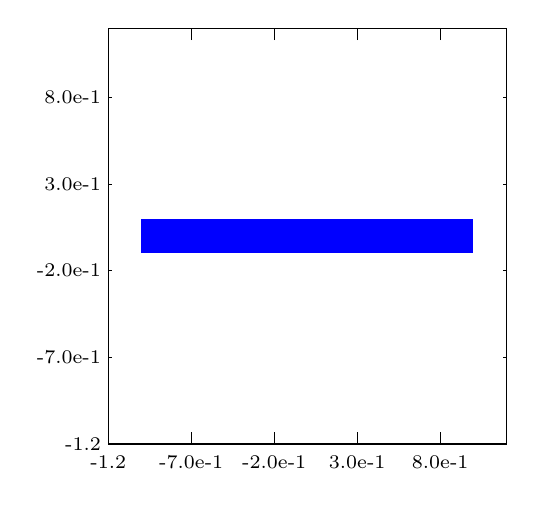
\begin{tikzpicture}[scale = 6,font=\scriptsize]
\draw (0.1148,0.085) rectangle (0.958,0.965);
\foreach \x/\label in {0.1148/-1.2,0.290466/-7.0e-1,0.466133/-2.0e-1,0.6418/3.0e-1,0.817466/8.0e-1} {
  \foreach \y in {0.94,0.085} \draw (\x,\y) -- (\x,\y+0.025);
  \node [below] at (\x,0.08) {\label};
}
\foreach \y/\label in {0.0849996/-1.2,0.268333/-7.0e-1,0.451666/-2.0e-1,0.635/3.0e-1,0.818333/8.0e-1} {
  \foreach \x in {0.951,0.1148} \draw (\x,\y) -- (\x+0.007,\y);
  \node [left] at (0.12,\y) {\label};
}
\fill [blue] (0.185067,0.488333) rectangle (0.887733,0.561667);
\end{tikzpicture}
\hspace{1cm}
% polygon
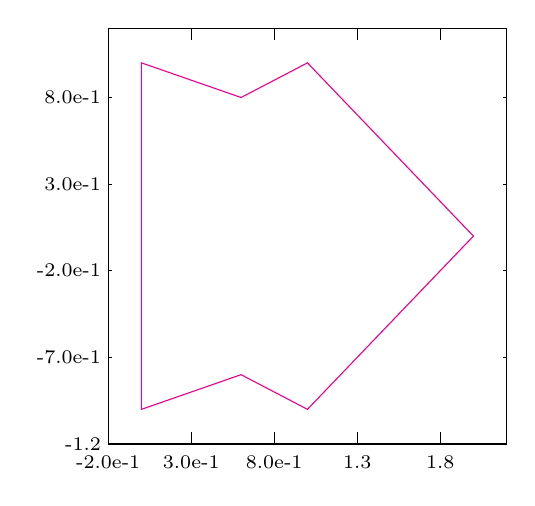
\begin{tikzpicture}[scale = 6,font=\scriptsize]
\draw (0.1148,0.085) rectangle (0.958,0.965);
\foreach \x/\label in {0.1148/-2.0e-1,0.290466/3.0e-1,0.466133/8.0e-1,0.6418/1.3,0.817466/1.8} {
  \foreach \y in {0.94,0.085} \draw (\x,\y) --(\x,\y+0.025);
  \node [below] at (\x,0.08) {\label};
}
\foreach \y/\label in {0.0849996/-1.2,0.268333/-7.0e-1,0.451666/-2.0e-1,0.635/3.0e-1,0.818333/8.0e-1} {
  \foreach \x in {0.951,0.1148} \draw (\x,\y) --(\x+0.007,\y);
  \node [left] at (0.12,\y) {\label};
}
\draw [magenta] (0.185067,0.891667) -- (0.185067,0.158333) -- (0.395867,0.231667) -- (0.5364,0.158333) -- (0.887733,0.525) -- (0.5364,0.891667) -- (0.395867,0.818333) -- cycle;
\end{tikzpicture}
\\[8mm]
% ellipse
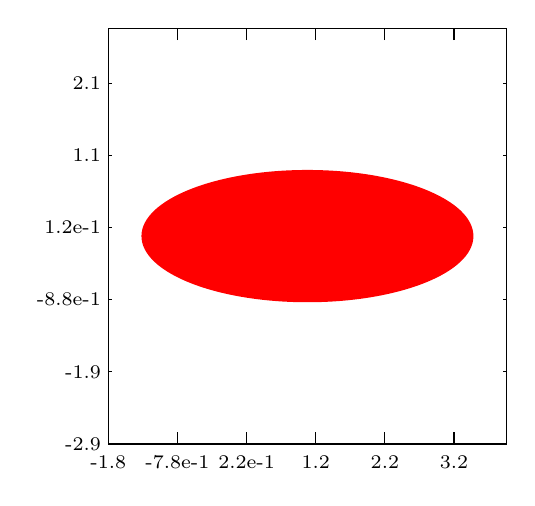
\begin{tikzpicture}[scale = 6,font=\scriptsize]
\draw (0.1148,0.085) rectangle (0.958,0.965);
\foreach \x/\label in {0.1148/-1.8,0.261189/-7.8e-1,0.407578/2.2e-1,0.553966/1.2,0.700355/2.2,0.846744/3.2} {
  \foreach \y in {0.94,0.085} \draw (\x,\y) --(\x,\y+0.025);
  \node [below] at (\x,0.08) {\label};
}
\foreach \y/\label in {0.0849996/-2.9,0.237777/-1.9,0.390555/-8.8e-1,0.543333/1.2e-1,0.696111/1.1,0.848888/2.1} {
  \foreach \x in {0.951,0.1148} \draw (\x,\y) --(\x+0.007,\y);
  \node [left] at (0.12,\y) {\label};
}
\fill [red] (0.5364,0.525) circle [x radius=0.351333,y radius=0.14];
\end{tikzpicture}
\hspace{1cm}
% ring
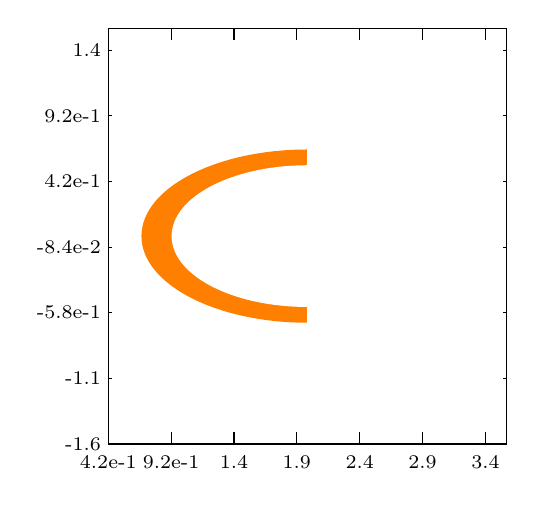
\begin{tikzpicture}[scale = 6,font=\scriptsize]
\draw (0.1148,0.085) rectangle (0.958,0.965);
\foreach \x/\label in {0.1148/4.2e-1,0.247881/9.2e-1,0.380962/1.4,0.514043/1.9,0.647123/2.4,0.780204/2.9,0.913285/3.4} {
  \foreach \y in {0.94,0.085} \draw (\x,\y) --(\x,\y+0.025);
  \node [below] at (\x,0.08) {\label};
}
\foreach \y/\label in {0.0849996/-1.6,0.223888/-1.1,0.362777/-5.8e-1,0.501666/-8.4e-2,0.640555/4.2e-1,0.779444/9.2e-1,0.918333/1.4} {
  \foreach \x in {0.951,0.1148} \draw (\x,\y) --(\x+0.007,\y);
  \node [left] at (0.12,\y) {\label};
}
\fill [color=orange] (0.5364,0.525) circle [x radius=0.351333,y radius=0.183333];
\fill [color=white] (0.5364,0.525) circle [x radius=0.287455,y radius=0.15];
\fill [color=white] (0.5364,0.158333) rectangle (0.9,0.784272);
\end{tikzpicture}
\caption{\label{fig:rg}Sample regions defined via the \ident{RG} class: interval (top left), polygon (top right), ellipse (bottom left), and ring (bottom right). These plots can be generated at run time by adding the command-line option \texttt{-rg\_view draw}.}
\end{figure}

Sometimes it is useful to specify the complement of a certain region, e.g., the part of the complex plane outside an ellipse. This can be achieved with
	\findex{RGSetComplement}
	\begin{Verbatim}[fontsize=\small]
        RGSetComplement(RG rg,PetscBool flg)
	\end{Verbatim}
or in the command line with \Verb!-rg_complement!.

By default, a newly created \ident{RG} object that is not set a type nor parameters must represent the whole complex plane (the same as \texttt{RGINTERVAL} with values $[-\infty,+\infty]\times[-\infty,+\infty]$). We call this the \emph{trivial} region, and provide a function to test this situation:
	\findex{RGIsTrivial}
	\begin{Verbatim}[fontsize=\small]
        RGIsTrivial(RG rg,PetscBool *trivial)
	\end{Verbatim}

Another useful operation is to check whether a given point of the complex plane is inside the region or not:
	\findex{RGCheckInside}
	\begin{Verbatim}[fontsize=\small]
        RGCheckInside(RG rg,PetscInt n,PetscScalar *ar,PetscScalar *ai,PetscInt *inside)
	\end{Verbatim}
Note that the point is represented as two \texttt{PetscScalar}'s, similarly to eigenvalues in \slepc.

\begin{table}
\centering
{\small \begin{tabular}{lll}
                       &                     & {\footnotesize Options} \\
Region Type            & \ident{RGType}      & {\footnotesize Database Name}\\\hline
(Generalized) Interval & \texttt{RGINTERVAL} & \texttt{interval} \\
Polygon                & \texttt{RGPOLYGON}  & \texttt{polygon} \\
Ellipse                & \texttt{RGELLIPSE}  & \texttt{ellipse} \\
Ring                   & \texttt{RGRING}     & \texttt{ring} \\\hline
\end{tabular} }
\caption{\label{tab:rg}Regions available as \ident{RG} objects.}
\end{table}

%---------------------------------------------------
\section{Directory Structure}

	The directory structure of the \slepc software is very similar to that in \petsc. The root directory of \slepc contains the following directories:
\begin{description}
\item[\texttt{lib/slepc/conf}] - Directory containing the base \slepc makefile, to be included in application makefiles.
\item[\texttt{config}] - \slepc configuration scripts.
\item[\texttt{docs}] - All documentation for \slepc, including this manual. The subdirectory \texttt{manualpages} contains the on-line manual pages of each \slepc routine.
\item[\texttt{include}] - All include files for \slepc. The following subdirectories exist:
\begin{description}
\setlength{\itemsep}{0mm}
\item[\texttt{slepc/finclude}] - include files for Fortran programmers.
\item[\texttt{slepc/private}] - include files containing implementation details, for developer use only.
\end{description}
\item[\texttt{share/slepc}] - Common files, including:
\begin{description}
\setlength{\itemsep}{0mm}
\item[\texttt{datafiles}] - data files used by some examples.
%\item[\texttt{matlab}] - Matlab interface and examples.
\end{description}
\item[\texttt{src}] - The source code for all \slepc components, which currently includes:
\begin{description}
\setlength{\itemsep}{0mm}
\item[\texttt{sys}] - system-related routines and auxiliary classes \texttt{bv}, \texttt{ds}, \texttt{fn}, \texttt{rg}, \texttt{st}.
\item[\texttt{eps}] - eigenvalue problem solver.
\item[\texttt{svd}] - singular value decomposition solver.
\item[\texttt{pep}] - polynomial eigenvalue problem solver.
\item[\texttt{nep}] - nonlinear eigenvalue problem solver.
\item[\texttt{mfn}] - matrix function.
\end{description}
\item[\texttt{\$PETSC\_ARCH}] - For each value of \ident{PETSC\_ARCH}, a directory exists containing files generated during installation of that particular configuration. The following subdirectories exist:
\begin{description}
\setlength{\itemsep}{0mm}
\item[\texttt{lib}] - all the generated libraries.
\item[\texttt{lib/slepc/conf}] - configuration parameters and log files.
\item[\texttt{include}] - automatically generated include files, such as Fortran 90 \texttt{*.mod} files.
\end{description}
\end{description}

Each \slepc source code component directory has the following subdirectories:
\begin{description}
\item[\texttt{interface}] - The calling sequences for the abstract interface to the components. Code here does not know about particular implementations.
\item[\texttt{impls}] - Source code for the different implementations.
\item[\texttt{examples}] - Example programs, classified in:
\begin{description}
\setlength{\itemsep}{0mm}
\item[\texttt{tutorials}] - examples intended for learning to use \slepc.
\item[\texttt{tests}] - examples used by testing scripts.
\end{description}
\end{description}

%---------------------------------------------------
%\section{Auxiliary Components}
%\label{sec:aux}

%The previous section includes a list of subdirectories, each of them representing a \slepc component. Most of these components have been treated in previous chapters. Here we include a brief report about two auxiliary components, \ident{BV} and \ident{DS}, that are not normally required by final users, but provide important operations to high level solvers such \ident{EPS}.

%\subsection{BV: Basis Vectors}

%\subsection{DS: Direct Solver (or Dense System)}

%---------------------------------------------------
\section{Wrappers to External Libraries}
\label{sec:wrap}

	\slepc interfaces to several external libraries for the solution of eigenvalue problems. This section provides a short description of each of these packages as well as some hints for using them with \slepc, including pointers to the respective websites from which the software can be downloaded. The description may also include method-specific parameters, that can be set in the same way as other \slepc options, either procedurally or via the command-line.

	In order to use \slepc together with an external library such as \arpack, one needs to do the following.
	\begin{enumerate}
	\item Install the external software, with the same compilers and MPI that will be used for \petsc/\slepc.
	\item Enable the utilization of the external software from \slepc by specifying configure options as explained in \S\ref{sec:opt-inst}.
 	\item Build the \slepc libraries.
	\item Use the runtime option \Verb!-eps_type <type>! to select the solver.
	\end{enumerate}

	Exceptions to the above rule are \lapack, which should be enabled during \petsc's configuration, and \blopex, that must be installed with \Verb!--download-blopex! in \slepc's configure. Other packages also support the download option.

\subsection*{\underline{\lapack}}
	\begin{description}
	\setlength{\itemsep}{0pt}
	\item[References.]\citep{Anderson:1992:LUG}.
	\item[Website.] \url{http://www.netlib.org/lapack}.
	\item[Version.] 3.0 or later.
	\item[Summary.] \lapack\ (Linear Algebra PACKage) is a software package for the solution of many different dense linear algebra problems, including various types of eigenvalue problems and singular value decompositions.

	\slepc explicitly creates the operator matrix in dense form and then the appropriate \lapack driver routine is invoked. Therefore, this interface should be used only for testing and validation purposes and not in a production code. The operator matrix is created by applying the operator to the columns of the identity matrix.

	\item[Installation.]
	The \slepc interface to \lapack can be used directly. If \slepc's configure script complains about missing \lapack functions, then configure \petsc with option \texttt{-{}-download-f2cblaslapack}.
	\end{description}

\subsection*{\underline{\arpack}}
	\begin{description}
	\setlength{\itemsep}{0pt}
	\item[References.]\citep{Lehoucq:1998:AUG}, \citep{Maschhoff:1996:PEP}.
	\item[Website.] \url{http://www.caam.rice.edu/software/ARPACK}.
	\item[Version.] Release 2 (plus patches).
	\item[Summary.] \arpack\ (ARnoldi PACKage) is a software package for the computation of a few eigenvalues and corresponding eigenvectors of a general $n\times n$ matrix $A$. It is most appropriate for large sparse or structured matrices, where structured means that a matrix-vector product $w \leftarrow Av$ requires order $n$ rather than the usual order $n^2$ floating point operations.
	
	\arpack\ is based upon an algorithmic variant of the Arnoldi process called the Implicitly Restarted Arnoldi Method (IRAM). When the matrix $A$ is symmetric it reduces to a variant of the Lanczos process called the Implicitly Restarted Lanczos Method (IRLM). These variants may be viewed as a synthesis of the Arnoldi/Lanczos process with the Implicitly Shifted QR technique that is suitable for large scale problems.

	It can be used for standard and generalized eigenvalue problems, both in real and complex arithmetic. It is implemented in Fortran 77 and it is based on the reverse communication interface. A parallel version, \parpack, is available with support for both MPI and BLACS.
	\item[Installation.]
	To install from the original website: first of all, unpack \texttt{arpack96.tar.gz} and also the patch file \texttt{patch.tar.gz}. If you plan to use the parallel version, extract also the contents of the file \texttt{parpack96.tar.gz} together with the patches \texttt{ppatch.tar.gz} (make sure you delete any \texttt{mpif.h} files that could exist in the directory tree). After setting all the directories, modify the \texttt{ARmake.inc} file and then compile the software with \texttt{make all}. It is recommended that \arpack is installed with its own \lapack version since it may give unexpected results with more recent versions of \lapack.

	Alternatively, one can use the \textsc{arpack-ng} distribution, available in \texttt{github.com}, that supports \texttt{configure}+\texttt{make} for installation. Also, \slepc's \texttt{configure} allows to download this version automatically via the \texttt{-{}-download-arpack} option.

	It is possible to configure \slepc with the serial version of \arpack. For this, you have to configure \petsc with the option \texttt{-{}-with-mpi=0}.
	\end{description}

\subsection*{\underline{\primme}}
	\begin{description}
	\setlength{\itemsep}{0pt}
	\item[References.]\citep{Stathopoulos:2010:PMS}.
	\item[Website.] \url{http://www.cs.wm.edu/~andreas/software}.
	\item[Version.] 2.1.
	\item[Summary.] \primme (PReconditioned Iterative MultiMethod Eigensolver) is a C library for finding a number of eigenvalues and their corresponding eigenvectors of a real symmetric (or complex Hermitian) matrix. This library provides a multimethod eigensolver, based on Davidson/Jacobi-Davidson. Particular methods include GD+1, JDQMR, and LOBPCG. It supports preconditioning as well as the computation of interior eigenvalues.
	\item[Installation.] Type \texttt{make lib} after customizing the file \texttt{Make\_flags} appropriately. Alternatively, the \texttt{-{}-download-primme} option is also available in \slepc's \texttt{configure}.
	\item[Specific options.] Since PRIMME contains preconditioned solvers, the \slepc interface uses \ident{STPRECOND}, as described in \ref{sec:precond}.

The \slepc interface to this package allows the user to specify the maximum allowed block size with the function \ident{EPSPRIMMESetBlockSize} or at run time with the option \Verb!-eps_primme_blocksize <size>!.
For changing the particular algorithm within \primme, use the function \ident{EPSPRIMMESetMethod}.

\primme also provides a solver for the singular value decomposition that is interfaced in \slepc's \ident{SVD}, see chapter \ref{cap:svd}.
	\end{description}

\subsection*{\underline{\blzpack}}
	\begin{description}
	\setlength{\itemsep}{0pt}
	\item[References.]\citep{Marques:1995:BDU}.
	\item[Website.] \url{http://crd.lbl.gov/\~osni/\#Software}.
	\item[Version.] 04/00.
	\item[Summary.] \blzpack\ (Block LancZos PACKage) is a standard Fortran 77 implementation of the block Lanczos algorithm intended for the solution of the standard eigenvalue problem $Ax=\mu x$ or the generalized eigenvalue problem $Ax=\mu Bx$, where A and B are real, sparse symmetric matrices. The development of this eigensolver was motivated by the need to solve large, sparse, generalized problems from free vibration analysis in structural engineering. Several upgrades were performed afterwards aiming at the solution of eigenvalue problems from a wider range of applications.

	\blzpack\ uses a combination of partial and selective re-orthogonalization strategies. It can be run in either sequential or parallel mode, by means of MPI or PVM interfaces, and it uses the reverse communication strategy.
	\item[Installation.] For the compilation of the \texttt{libblzpack.a} library, first check the appropriate architecture file in the directory \texttt{sys/MACROS} and then type \texttt{creator -mpi}.
	\item[Specific options.] The \slepc interface to this package allows the user to specify the block size with the function \ident{EPSBlzpackSetBlockSize} or at run time with the option \Verb!-eps_blzpack_! \Verb!blocksize <size>!. Also, the function \ident{EPSBlzpackSetNSteps} can be used to set the maximum number of steps per run (also with \Verb!-eps_blzpack_nsteps!).
	\end{description}

\subsection*{\underline{\trlan}}
	\begin{description}
	\setlength{\itemsep}{0pt}
	\item[References.]\citep{Wu:2000:TLM}.
	\item[Website.] \url{http://crd.lbl.gov/\~kewu/trlan.html}.
	\item[Version.] 201009.
	\item[Summary.] This package provides a Fortran 90 implementation of the dynamic thick-restart Lanczos algorithm. This is a specialized version of Lanczos that targets only the case in which one wants both eigenvalues and eigenvectors of a large real symmetric eigenvalue problem that cannot use the shift-and-invert scheme. In this case the standard non-restarted Lanczos algorithm requires to store a large number of Lanczos vectors, what can cause storage problems and make each iteration of the method very expensive.

	\trlan{} requires the user to provide a matrix-vector multiplication routine. The parallel version uses MPI as the message passing layer.
	\item[Installation.] To install this package, it is necessary to have access to a Fortran 90 compiler. The compiler name and the options used are specified in the file called \texttt{Make.inc}. To generate the library, type \texttt{make plib} in the \texttt{TRLan} directory. Alternatively, the \texttt{-{}-download-trlan} option is also available in \slepc's \texttt{configure}.

	It is possible to configure \slepc with the serial version of \trlan (built with \texttt{make lib}). For this, you have to configure \petsc with the option \texttt{-{}-with-mpi=0}.
	\end{description}

\subsection*{\underline{\blopex}}
	\begin{description}
	\setlength{\itemsep}{0pt}
	\item[References.]\citep{Knyazev:2007:BLO}.
	\item[Website.] \url{http://bitbucket.org/joseroman/blopex}.
	\item[Summary.] \blopex is a package that implements the Locally Optimal Block Preconditioned Conjugate Gradient (LOBPCG) method for computing several extreme eigenpairs of symmetric positive generalized eigenproblems. Numerical comparisons suggest that this method is a genuine analog for eigenproblems of the standard preconditioned conjugate gradient method for symmetric linear systems.
	\item[Installation.] In order to use \blopex from \slepc, it necessary to install it during \slepc's configuration: \Verb!./configure --download-blopex!.
	\item[Specific options.] Since BLOPEX contains preconditioned solvers, the \slepc interface uses \ident{STPRECOND}, as described in \ref{sec:precond}.
	\end{description}

\subsection*{\underline{\feast}}
	\begin{description}
	\setlength{\itemsep}{0pt}
	\item[References.]\citep{Polizzi:2009:DAS}.
	\item[Website.] \url{http://www.ecs.umass.edu/~polizzi/feast}.
	\item[Summary.] \feast is a numerical library for solving the standard or generalized symmetric eigenvalue problem, and obtaining all the eigenvalues and eigenvectors within a given search interval. It is based on an innovative fast and stable numerical algorithm which deviates fundamentally from the traditional Krylov subspace based iterations or Davidson-Jacobi techniques. The FEAST algorithm takes its inspiration from the density-matrix representation and contour integration technique in quantum mechanics.
	\item[Specific options.] The \slepc interface to \feast allows the user to specify the number of contour integration points with the function \ident{EPSFEASTSetNumPoints} or at run time with the option \Verb!-eps_feast_num_points <n>!.
	\end{description}

%---------------------------------------------------
\section{Fortran Interface}
\label{sec:fortran}

	\slepc provides an interface for Fortran programmers, very much like \petsc. As in the case of \petsc, there are slight differences between the C and Fortran \slepc interfaces, due to differences in Fortran syntax. For instance, the error checking variable is the final argument of all the routines in the Fortran interface, in contrast to the C convention of providing the error variable as the routine's return value.

	The following is a Fortran example with fixed-format source. It is the Fortran equivalent of the program given in \S\ref{sec:simpleex} and can be found in \Verb!${SLEPC_DIR}/src/eps/examples/tutorials! (file \texttt{ex1f.F}). It is also possible to use free-format source (see \texttt{ex1f90.F90}).
\MyVerbatimInput{ex1f.F}

%---------------------------------------------------
%\section{Matlab Interface}
%\label{sec:matlab}
%
%Since version 3.2, \slepc includes an interface intended to make most of \slepc's functionality available from Matlab. It is experimental and needs further development, so users planning to use it seriously are recommended to contact the authors. Below are some guidelines for using this interface.
%
%First of all, \petsc must have been configured with the Matlab interface enabled. This can be done as follows (check \petsc documentation for details):
%	\begin{Verbatim}[fontsize=\small]
%	$ ./configure --with-matlab --with-matlab-engine --with-shared-libraries
%	\end{Verbatim}
%
%Once the \petsc and \slepc libraries have been built, one has to set Matlab's path to point to the directories containing Matlab classes: \Verb!$SLEPC_DIR/share/slepc/matlab/classes! and \Verb!$PETSC_DIR/share/slepc/matlab/classes!. Below we show a simple Matlab example (included in \slepc's distribution) that does this, and then solves a simple eigenproblem.
%\MyVerbatimInput{exEPS.m}



%---------------------------------------------------
\cleardoublepage
\fancyhead{}\fancyhead[LO,RE]{\nouppercase{\scriptsize \sffamily Bibliography}}
\addcontentsline{toc}{chapter}{Bibliography}

%\bibliographystyle{engnat}
%\bibliography{slepc}
%%
%% This is file `slepc.cls',
%% 
%% This file is based on book.cls.
%% 
%% Copyright 1993 1994 1995 1996 1997 1998 1999
%% The LaTeX3 Project and any individual authors listed elsewhere
%% in this file.
%% 
%% This file is part of the LaTeX2e system.
%% ----------------------------------------
%% 
%% It may be distributed under the terms of the LaTeX Project Public
%% License, as described in lppl.txt in the base LaTeX distribution.
%% Either version 1.0 or, at your option, any later version.
%% \CharacterTable
%%  {Upper-case    \A\B\C\D\E\F\G\H\I\J\K\L\M\N\O\P\Q\R\S\T\U\V\W\X\Y\Z
%%   Lower-case    \a\b\c\d\e\f\g\h\i\j\k\l\m\n\o\p\q\r\s\t\u\v\w\x\y\z
%%   Digits        \0\1\2\3\4\5\6\7\8\9
%%   Exclamation   \!     Double quote  \"     Hash (number) \#
%%   Dollar        \$     Percent       \%     Ampersand     \&
%%   Acute accent  \'     Left paren    \(     Right paren   \)
%%   Asterisk      \*     Plus          \+     Comma         \,
%%   Minus         \-     Point         \.     Solidus       \/
%%   Colon         \:     Semicolon     \;     Less than     \<
%%   Equals        \=     Greater than  \>     Question mark \?
%%   Commercial at \@     Left bracket  \[     Backslash     \\
%%   Right bracket \]     Circumflex    \^     Underscore    \_
%%   Grave accent  \`     Left brace    \{     Vertical bar  \|
%%   Right brace   \}     Tilde         \~}
\NeedsTeXFormat{LaTeX2e}[1995/12/01]
\ProvidesClass{slepc}
              [1999/01/07 v1.4a
 Standard LaTeX document class]
\newcommand\@ptsize{}
\newif\if@restonecol
\newif\if@titlepage
\@titlepagetrue
\newif\if@openright
\newif\if@mainmatter \@mainmattertrue
\if@compatibility\else
\DeclareOption{a4paper}
   {\setlength\paperheight {297mm}%
    \setlength\paperwidth  {210mm}}
\DeclareOption{a5paper}
   {\setlength\paperheight {210mm}%
    \setlength\paperwidth  {148mm}}
\DeclareOption{b5paper}
   {\setlength\paperheight {250mm}%
    \setlength\paperwidth  {176mm}}
\DeclareOption{letterpaper}
   {\setlength\paperheight {11in}%
    \setlength\paperwidth  {8.5in}}
\DeclareOption{legalpaper}
   {\setlength\paperheight {14in}%
    \setlength\paperwidth  {8.5in}}
\DeclareOption{executivepaper}
   {\setlength\paperheight {10.5in}%
    \setlength\paperwidth  {7.25in}}
\DeclareOption{landscape}
   {\setlength\@tempdima   {\paperheight}%
    \setlength\paperheight {\paperwidth}%
    \setlength\paperwidth  {\@tempdima}}
\fi
\if@compatibility
  \renewcommand\@ptsize{0}
\else
\DeclareOption{10pt}{\renewcommand\@ptsize{0}}
\fi
\DeclareOption{11pt}{\renewcommand\@ptsize{1}}
\DeclareOption{12pt}{\renewcommand\@ptsize{2}}
\if@compatibility\else
\DeclareOption{oneside}{\@twosidefalse \@mparswitchfalse}
\fi
\DeclareOption{twoside}{\@twosidetrue  \@mparswitchtrue}
\DeclareOption{draft}{\setlength\overfullrule{5pt}}
\if@compatibility\else
\DeclareOption{final}{\setlength\overfullrule{0pt}}
\fi
\DeclareOption{titlepage}{\@titlepagetrue}
\if@compatibility\else
\DeclareOption{notitlepage}{\@titlepagefalse}
\fi
\if@compatibility
\@openrighttrue
\else
\DeclareOption{openright}{\@openrighttrue}
\DeclareOption{openany}{\@openrightfalse}
\fi
\if@compatibility\else
\DeclareOption{onecolumn}{\@twocolumnfalse}
\fi
\DeclareOption{twocolumn}{\@twocolumntrue}
\DeclareOption{leqno}{\input{leqno.clo}}
\DeclareOption{fleqn}{\input{fleqn.clo}}
\DeclareOption{openbib}{%
  \AtEndOfPackage{%
   \renewcommand\@openbib@code{%
      \advance\leftmargin\bibindent
      \itemindent -\bibindent
      \listparindent \itemindent
      \parsep \z@
      }%
   \renewcommand\newblock{\par}}%
}
\ExecuteOptions{letterpaper,10pt,twoside,onecolumn,final,openright}
\ProcessOptions
\input{bk1\@ptsize.clo}
\setlength\lineskip{1\p@}
\setlength\normallineskip{1\p@}
\renewcommand\baselinestretch{}
\setlength\parskip{0\p@ \@plus \p@}
\@lowpenalty   51
\@medpenalty  151
\@highpenalty 301
\setcounter{topnumber}{2}
\renewcommand\topfraction{.7}
\setcounter{bottomnumber}{1}
\renewcommand\bottomfraction{.3}
\setcounter{totalnumber}{3}
\renewcommand\textfraction{.2}
\renewcommand\floatpagefraction{.5}
\setcounter{dbltopnumber}{2}
\renewcommand\dbltopfraction{.7}
\renewcommand\dblfloatpagefraction{.5}
\if@twoside
  \def\ps@headings{%
      \let\@oddfoot\@empty\let\@evenfoot\@empty
      \def\@evenhead{\thepage\hfil\slshape\leftmark}%
      \def\@oddhead{{\slshape\rightmark}\hfil\thepage}%
      \let\@mkboth\markboth
    \def\chaptermark##1{%
      \markboth {\MakeUppercase{%
        \ifnum \c@secnumdepth >\m@ne
          \if@mainmatter
            \@chapapp\ \thechapter. \ %
          \fi
        \fi
        ##1}}{}}%
    \def\sectionmark##1{%
      \markright {\MakeUppercase{%
        \ifnum \c@secnumdepth >\z@
          \thesection. \ %
        \fi
        ##1}}}}
\else
  \def\ps@headings{%
    \let\@oddfoot\@empty
    \def\@oddhead{{\slshape\rightmark}\hfil\thepage}%
    \let\@mkboth\markboth
    \def\chaptermark##1{%
      \markright {\MakeUppercase{%
        \ifnum \c@secnumdepth >\m@ne
          \if@mainmatter
            \@chapapp\ \thechapter. \ %
          \fi
        \fi
        ##1}}}}
\fi
\def\ps@myheadings{%
    \let\@oddfoot\@empty\let\@evenfoot\@empty
    \def\@evenhead{\thepage\hfil\slshape\leftmark}%
    \def\@oddhead{{\slshape\rightmark}\hfil\thepage}%
    \let\@mkboth\@gobbletwo
    \let\chaptermark\@gobble
    \let\sectionmark\@gobble
    }
  \if@titlepage
  \newcommand\maketitle{\begin{titlepage}%
  \let\footnotesize\small
  \let\footnoterule\relax
  \let \footnote \thanks
  \null\vfil
  \vskip 60\p@
  \begin{center}%
    {\LARGE \@title \par}%
    \vskip 3em%
    {\large
     \lineskip .75em%
      \begin{tabular}[t]{c}%
        \@author
      \end{tabular}\par}%
      \vskip 1.5em%
    {\large \@date \par}%       % Set date in \large size.
  \end{center}\par
  \@thanks
  \vfil\null
  \end{titlepage}%
  \setcounter{footnote}{0}%
  \global\let\thanks\relax
  \global\let\maketitle\relax
  \global\let\@thanks\@empty
  \global\let\@author\@empty
  \global\let\@date\@empty
  \global\let\@title\@empty
  \global\let\title\relax
  \global\let\author\relax
  \global\let\date\relax
  \global\let\and\relax
}
\else
\newcommand\maketitle{\par
  \begingroup
    \renewcommand\thefootnote{\@fnsymbol\c@footnote}%
    \def\@makefnmark{\rlap{\@textsuperscript{\normalfont\@thefnmark}}}%
    \long\def\@makefntext##1{\parindent 1em\noindent
            \hb@xt@1.8em{%
                \hss\@textsuperscript{\normalfont\@thefnmark}}##1}%
    \if@twocolumn
      \ifnum \col@number=\@ne
        \@maketitle
      \else
        \twocolumn[\@maketitle]%
      \fi
    \else
      \newpage
      \global\@topnum\z@   % Prevents figures from going at top of page.
      \@maketitle
    \fi
    \thispagestyle{plain}\@thanks
  \endgroup
  \setcounter{footnote}{0}%
  \global\let\thanks\relax
  \global\let\maketitle\relax
  \global\let\@maketitle\relax
  \global\let\@thanks\@empty
  \global\let\@author\@empty
  \global\let\@date\@empty
  \global\let\@title\@empty
  \global\let\title\relax
  \global\let\author\relax
  \global\let\date\relax
  \global\let\and\relax
}
\def\@maketitle{%
  \newpage
  \null
  \vskip 2em%
  \begin{center}%
  \let \footnote \thanks
    {\LARGE \@title \par}%
    \vskip 1.5em%
    {\large
      \lineskip .5em%
      \begin{tabular}[t]{c}%
        \@author
      \end{tabular}\par}%
    \vskip 1em%
    {\large \@date}%
  \end{center}%
  \par
  \vskip 1.5em}
\fi
\newcommand*\chaptermark[1]{}
\setcounter{secnumdepth}{2}
\newcounter {part}
\newcounter {chapter}
\newcounter {section}[chapter]
\newcounter {subsection}[section]
\newcounter {subsubsection}[subsection]
\newcounter {paragraph}[subsubsection]
\newcounter {subparagraph}[paragraph]
\renewcommand \thepart {\@Roman\c@part}
\renewcommand \thechapter {\@arabic\c@chapter}
\renewcommand \thesection {\thechapter.\@arabic\c@section}
\renewcommand\thesubsection   {\thesection.\@arabic\c@subsection}
\renewcommand\thesubsubsection{\thesubsection .\@arabic\c@subsubsection}
\renewcommand\theparagraph    {\thesubsubsection.\@arabic\c@paragraph}
\renewcommand\thesubparagraph {\theparagraph.\@arabic\c@subparagraph}
\newcommand\@chapapp{\chaptername}
\newcommand\frontmatter{%
    \cleardoublepage
  \@mainmatterfalse
  \pagenumbering{roman}}
\newcommand\mainmatter{%
    \cleardoublepage
  \@mainmattertrue
  \pagenumbering{arabic}}
\newcommand\backmatter{%
  \if@openright
    \cleardoublepage
  \else
    \clearpage
  \fi
  \@mainmatterfalse}
\newcommand\part{%
  \if@openright
    \cleardoublepage
  \else
    \clearpage
  \fi
  \thispagestyle{plain}%
  \if@twocolumn
    \onecolumn
    \@tempswatrue
  \else
    \@tempswafalse
  \fi
  \null\vfil
  \secdef\@part\@spart}

\def\@part[#1]#2{%
    \ifnum \c@secnumdepth >-2\relax
      \refstepcounter{part}%
      \addcontentsline{toc}{part}{\thepart\hspace{1em}#1}%
    \else
      \addcontentsline{toc}{part}{#1}%
    \fi
    \markboth{}{}%
    {\centering
     \interlinepenalty \@M
     \normalfont
     \ifnum \c@secnumdepth >-2\relax
       \huge\bfseries \partname~\thepart
       \par
       \vskip 20\p@
     \fi
     \Huge \bfseries #2\par}%
    \@endpart}
\def\@spart#1{%
    {\centering
     \interlinepenalty \@M
     \normalfont
     \Huge \bfseries #1\par}%
    \@endpart}
\def\@endpart{\vfil\newpage
              \if@twoside
                \null
                \thispagestyle{empty}%
                \newpage
              \fi
              \if@tempswa
                \twocolumn
              \fi}
\newcommand\chapter{\if@openright\cleardoublepage\else\clearpage\fi
                    \thispagestyle{plain}%
                    \global\@topnum\z@
                    \@afterindentfalse
                    \secdef\@chapter\@schapter}
\def\@chapter[#1]#2{\ifnum \c@secnumdepth >\m@ne
                       \if@mainmatter
                         \refstepcounter{chapter}%
%                         \typeout{\@chapapp\space\thechapter.}%
\typeout{--------------\space Capitulo\space\thechapter\space--------------}
                         \addcontentsline{toc}{chapter}%
                                   {\protect\numberline{\thechapter}#1}%
                       \else
                         \addcontentsline{toc}{chapter}{#1}%
                       \fi
                    \else
                      \addcontentsline{toc}{chapter}{#1}%
                    \fi
                    \chaptermark{#1}%
                    \addtocontents{lof}{\protect\addvspace{10\p@}}%
                    \addtocontents{lot}{\protect\addvspace{10\p@}}%
                    \if@twocolumn
                      \@topnewpage[\@makechapterhead{#2}]%
                    \else
                      \@makechapterhead{#2}%
                      \@afterheading
                    \fi}
\def\@makechapterhead#1{%
  \vspace*{50\p@}%
%  {\parindent \z@ \raggedright \normalfont
  {\parindent \z@ \raggedleft \normalfont
    \ifnum \c@secnumdepth >\m@ne
      \if@mainmatter
%        \huge\bfseries \@chapapp\space \thechapter
%        \par\nobreak
%        \vskip 20\p@
\setlength{\fboxsep}{2mm}\fbox{\large\sc\@chapapp}\hspace*{-1.5mm}
\setlength{\fboxsep}{4mm}\setlength{\fboxrule}{.5mm}\fbox{\Huge\bfseries\thechapter} \par \raggedright
        \vskip 40\p@
      \fi
    \fi
    \interlinepenalty\@M
%    \Huge \bfseries #1\par\nobreak
%    \vskip 40\p@
    \huge\bf\sffamily #1\par\nobreak
    \hfill\rule{10cm}{1pt}
    \vskip 30\p@
  }}
\def\@schapter#1{\if@twocolumn
                   \@topnewpage[\@makeschapterhead{#1}]%
                 \else
                   \@makeschapterhead{#1}%
                   \@afterheading
                 \fi}
\def\@makeschapterhead#1{%
  \vspace*{50\p@}%
  {\parindent \z@ \raggedright
    \normalfont
    \interlinepenalty\@M
    \Huge \bfseries  #1\par\nobreak
    \vskip 40\p@
  }}
\newcommand\section{\@startsection {section}{1}{\z@}%
                                   {-3.5ex \@plus -1ex \@minus -.2ex}%
                                   {2.3ex \@plus.2ex}%
                                   {\normalfont\Large\bfseries}}
\newcommand\subsection{\@startsection{subsection}{2}{\z@}%
                                     {-3.25ex\@plus -1ex \@minus -.2ex}%
                                     {1.5ex \@plus .2ex}%
                                     {\normalfont\large\bfseries}}
\newcommand\subsubsection{\@startsection{subsubsection}{3}{\z@}%
                                     {-3.25ex\@plus -1ex \@minus -.2ex}%
                                     {1.5ex \@plus .2ex}%
                                     {\normalfont\normalsize\bfseries}}
\newcommand\paragraph{\@startsection{paragraph}{4}{\z@}%
                                    {3.25ex \@plus1ex \@minus.2ex}%
                                    {-1em}%
                                    {\normalfont\normalsize\bfseries}}
\newcommand\subparagraph{\@startsection{subparagraph}{5}{\parindent}%
                                       {3.25ex \@plus1ex \@minus .2ex}%
                                       {-1em}%
                                      {\normalfont\normalsize\bfseries}}
\if@twocolumn
  \setlength\leftmargini  {2em}
\else
  \setlength\leftmargini  {2.5em}
\fi
\leftmargin  \leftmargini
\setlength\leftmarginii  {2.2em}
\setlength\leftmarginiii {1.87em}
\setlength\leftmarginiv  {1.7em}
\if@twocolumn
  \setlength\leftmarginv  {.5em}
  \setlength\leftmarginvi {.5em}
\else
  \setlength\leftmarginv  {1em}
  \setlength\leftmarginvi {1em}
\fi
\setlength  \labelsep  {.5em}
\setlength  \labelwidth{\leftmargini}
\addtolength\labelwidth{-\labelsep}
\@beginparpenalty -\@lowpenalty
\@endparpenalty   -\@lowpenalty
\@itempenalty     -\@lowpenalty
\renewcommand\theenumi{\@arabic\c@enumi}
\renewcommand\theenumii{\@alph\c@enumii}
\renewcommand\theenumiii{\@roman\c@enumiii}
\renewcommand\theenumiv{\@Alph\c@enumiv}
\newcommand\labelenumi{\theenumi.}
\newcommand\labelenumii{(\theenumii)}
\newcommand\labelenumiii{\theenumiii.}
\newcommand\labelenumiv{\theenumiv.}
\renewcommand\p@enumii{\theenumi}
\renewcommand\p@enumiii{\theenumi(\theenumii)}
\renewcommand\p@enumiv{\p@enumiii\theenumiii}
\newcommand\labelitemi{\textbullet}
\newcommand\labelitemii{\normalfont\bfseries \textendash}
\newcommand\labelitemiii{\textasteriskcentered}
\newcommand\labelitemiv{\textperiodcentered}
\newenvironment{description}
               {\list{}{\labelwidth\z@ \itemindent-\leftmargin
                        \let\makelabel\descriptionlabel}}
               {\endlist}
\newcommand*\descriptionlabel[1]{\hspace\labelsep
                                \normalfont\bfseries #1}
\newenvironment{verse}
               {\let\\\@centercr
                \list{}{\itemsep      \z@
                        \itemindent   -1.5em%
                        \listparindent\itemindent
                        \rightmargin  \leftmargin
                        \advance\leftmargin 1.5em}%
                \item\relax}
               {\endlist}
\newenvironment{quotation}
               {\list{}{\listparindent 1.5em%
                        \itemindent    \listparindent
                        \rightmargin   \leftmargin
                        \parsep        \z@ \@plus\p@}%
                \item\relax}
               {\endlist}
\newenvironment{quote}
               {\list{}{\rightmargin\leftmargin}%
                \item\relax}
               {\endlist}
\if@compatibility
\newenvironment{titlepage}
    {%
      \cleardoublepage
      \if@twocolumn
        \@restonecoltrue\onecolumn
      \else
        \@restonecolfalse\newpage
      \fi
      \thispagestyle{empty}%
      \setcounter{page}\z@
    }%
    {\if@restonecol\twocolumn \else \newpage \fi
    }
\else
\newenvironment{titlepage}
    {%
      \cleardoublepage
      \if@twocolumn
        \@restonecoltrue\onecolumn
      \else
        \@restonecolfalse\newpage
      \fi
      \thispagestyle{empty}%
      \setcounter{page}\@ne
    }%
    {\if@restonecol\twocolumn \else \newpage \fi
     \if@twoside\else
        \setcounter{page}\@ne
     \fi
    }
\fi
\newcommand\appendix{\par
  \setcounter{chapter}{0}%
  \setcounter{section}{0}%
  \gdef\@chapapp{\appendixname}%
  \gdef\thechapter{\@Alph\c@chapter}}
\setlength\arraycolsep{5\p@}
\setlength\tabcolsep{6\p@}
\setlength\arrayrulewidth{.4\p@}
\setlength\doublerulesep{2\p@}
\setlength\tabbingsep{\labelsep}
\skip\@mpfootins = \skip\footins
\setlength\fboxsep{3\p@}
\setlength\fboxrule{.4\p@}
\@addtoreset {equation}{chapter}
\renewcommand\theequation
  {\ifnum \c@chapter>\z@ \thechapter.\fi \@arabic\c@equation}
\newcounter{figure}[chapter]
\renewcommand \thefigure
     {\ifnum \c@chapter>\z@ \thechapter.\fi \@arabic\c@figure}
\def\fps@figure{tbp}
\def\ftype@figure{1}
\def\ext@figure{lof}
\def\fnum@figure{\figurename~\thefigure}
\newenvironment{figure}
               {\@float{figure}}
               {\end@float}
\newenvironment{figure*}
               {\@dblfloat{figure}}
               {\end@dblfloat}
\newcounter{table}[chapter]
\renewcommand \thetable
     {\ifnum \c@chapter>\z@ \thechapter.\fi \@arabic\c@table}
\def\fps@table{tbp}
\def\ftype@table{2}
\def\ext@table{lot}
\def\fnum@table{\tablename~\thetable}
\newenvironment{table}
               {\@float{table}}
               {\end@float}
\newenvironment{table*}
               {\@dblfloat{table}}
               {\end@dblfloat}
\newlength\abovecaptionskip
\newlength\belowcaptionskip
\setlength\abovecaptionskip{10\p@}
\setlength\belowcaptionskip{0\p@}
\long\def\@makecaption#1#2{%
  \vskip\abovecaptionskip
  \sbox\@tempboxa{#1: #2}%
  \ifdim \wd\@tempboxa >\hsize
    #1: #2\par
  \else
    \global \@minipagefalse
    \hb@xt@\hsize{\hfil\box\@tempboxa\hfil}%
  \fi
  \vskip\belowcaptionskip}
\DeclareOldFontCommand{\rm}{\normalfont\rmfamily}{\mathrm}
\DeclareOldFontCommand{\sf}{\normalfont\sffamily}{\mathsf}
\DeclareOldFontCommand{\tt}{\normalfont\ttfamily}{\mathtt}
\DeclareOldFontCommand{\bf}{\normalfont\bfseries}{\mathbf}
\DeclareOldFontCommand{\it}{\normalfont\itshape}{\mathit}
\DeclareOldFontCommand{\sl}{\normalfont\slshape}{\@nomath\sl}
\DeclareOldFontCommand{\sc}{\normalfont\scshape}{\@nomath\sc}
\DeclareRobustCommand*\cal{\@fontswitch\relax\mathcal}
\DeclareRobustCommand*\mit{\@fontswitch\relax\mathnormal}
\newcommand\@pnumwidth{1.55em}
\newcommand\@tocrmarg{2.55em}
\newcommand\@dotsep{4.5}
\setcounter{tocdepth}{2}
\newcommand\tableofcontents{%
    \if@twocolumn
      \@restonecoltrue\onecolumn
    \else
      \@restonecolfalse
    \fi
    \chapter*{\contentsname
        \@mkboth{%
           \MakeUppercase\contentsname}{\MakeUppercase\contentsname}}%
    \@starttoc{toc}%
    \if@restonecol\twocolumn\fi
    }
\newcommand*\l@part[2]{%
  \ifnum \c@tocdepth >-2\relax
    \addpenalty{-\@highpenalty}%
    \addvspace{2.25em \@plus\p@}%
    \begingroup
      \parindent \z@ \rightskip \@pnumwidth
      \parfillskip -\@pnumwidth
      {\leavevmode
       \large \bfseries #1\hfil \hb@xt@\@pnumwidth{\hss #2}}\par
       \nobreak
         \global\@nobreaktrue
         \everypar{\global\@nobreakfalse\everypar{}}%
    \endgroup
  \fi}
\newcommand*\l@chapter[2]{%
  \ifnum \c@tocdepth >\m@ne
    \addpenalty{-\@highpenalty}%
    \vskip 1.0em \@plus\p@
    \setlength\@tempdima{1.5em}%
    \begingroup
      \parindent \z@ \rightskip \@pnumwidth
      \parfillskip -\@pnumwidth
      \leavevmode \bfseries
      \advance\leftskip\@tempdima
      \hskip -\leftskip
      #1\nobreak\hfil \nobreak\hb@xt@\@pnumwidth{\hss #2}\par
      \penalty\@highpenalty
    \endgroup
  \fi}
\newcommand*\l@section{\@dottedtocline{1}{1.5em}{2.3em}}
\newcommand*\l@subsection{\@dottedtocline{2}{3.8em}{3.2em}}
\newcommand*\l@subsubsection{\@dottedtocline{3}{7.0em}{4.1em}}
\newcommand*\l@paragraph{\@dottedtocline{4}{10em}{5em}}
\newcommand*\l@subparagraph{\@dottedtocline{5}{12em}{6em}}
\newcommand\listoffigures{%
    \if@twocolumn
      \@restonecoltrue\onecolumn
    \else
      \@restonecolfalse
    \fi
    \chapter*{\listfigurename
      \@mkboth{\MakeUppercase\listfigurename}%
              {\MakeUppercase\listfigurename}}%
    \@starttoc{lof}%
    \if@restonecol\twocolumn\fi
    }
\newcommand*\l@figure{\@dottedtocline{1}{1.5em}{2.3em}}
\newcommand\listoftables{%
    \if@twocolumn
      \@restonecoltrue\onecolumn
    \else
      \@restonecolfalse
    \fi
    \chapter*{\listtablename
      \@mkboth{%
          \MakeUppercase\listtablename}{\MakeUppercase\listtablename}}%
    \@starttoc{lot}%
    \if@restonecol\twocolumn\fi
    }
\let\l@table\l@figure
\newdimen\bibindent
\setlength\bibindent{1.5em}
\newenvironment{thebibliography}[1]
     {\chapter*{\bibname
        \@mkboth{\MakeUppercase\bibname}{\MakeUppercase\bibname}}%
      \list{\@biblabel{\@arabic\c@enumiv}}%
           {\settowidth\labelwidth{\@biblabel{#1}}%
            \leftmargin\labelwidth
            \advance\leftmargin\labelsep
            \@openbib@code
            \usecounter{enumiv}%
            \let\p@enumiv\@empty
            \renewcommand\theenumiv{\@arabic\c@enumiv}}%
      \sloppy
      \clubpenalty4000
      \@clubpenalty \clubpenalty
      \widowpenalty4000%
      \sfcode`\.\@m}
     {\def\@noitemerr
       {\@latex@warning{Empty `thebibliography' environment}}%
      \endlist}
\newcommand\newblock{\hskip .11em\@plus.33em\@minus.07em}
\let\@openbib@code\@empty
\newenvironment{theindex}
               {\if@twocolumn
                  \@restonecolfalse
                \else
                  \@restonecoltrue
                \fi
                \columnseprule \z@
                \columnsep 35\p@
                \twocolumn[\@makeschapterhead{\indexname}]%
                \@mkboth{\MakeUppercase\indexname}%
                        {\MakeUppercase\indexname}%
                \thispagestyle{plain}\parindent\z@
                \parskip\z@ \@plus .3\p@\relax
                \let\item\@idxitem}
               {\if@restonecol\onecolumn\else\clearpage\fi}
\newcommand\@idxitem{\par\hangindent 40\p@}
\newcommand\subitem{\@idxitem \hspace*{20\p@}}
\newcommand\subsubitem{\@idxitem \hspace*{30\p@}}
\newcommand\indexspace{\par \vskip 10\p@ \@plus5\p@ \@minus3\p@\relax}
\renewcommand\footnoterule{%
  \kern-3\p@
  \hrule\@width.4\columnwidth
  \kern2.6\p@}
\@addtoreset{footnote}{chapter}
\newcommand\@makefntext[1]{%
    \parindent 1em%
    \noindent
    \hb@xt@1.8em{\hss\@makefnmark}#1}
\newcommand\contentsname{Contents}
\newcommand\listfigurename{List of Figures}
\newcommand\listtablename{List of Tables}
\newcommand\bibname{Bibliography}
\newcommand\indexname{Index}
\newcommand\figurename{Figure}
\newcommand\tablename{Table}
\newcommand\partname{Part}
\newcommand\chaptername{Chapter}
\newcommand\appendixname{Appendix}
\def\today{\ifcase\month\or
  January\or February\or March\or April\or May\or June\or
  July\or August\or September\or October\or November\or December\fi
  \space\number\day, \number\year}
\setlength\columnsep{10\p@}
\setlength\columnseprule{0\p@}
\pagestyle{headings}
\pagenumbering{arabic}
\if@twoside
\else
  \raggedbottom
\fi
\if@twocolumn
  \twocolumn
  \sloppy
  \flushbottom
\else
  \onecolumn
\fi
\endinput
%%
%% End of file `slepc.cls'.


{\bibfont
\paragraph{SLEPc Technical Reports}
\hypertarget{str}{}
(Note: these reports are available through the \href{http://slepc.upv.es}{\slepc web site}.)
\begin{list}{}{\setlength{\labelwidth}{3cm}\setlength{\leftmargin}{12.5mm}}
\item[\textrm{\sffamily[STR-1]}] V. Hern\'andez, J. E. Rom\'an, A. Tom\'as, V. Vidal. ``Orthogonalization Routines in \slepc.'' 
\item[\textrm{\sffamily[STR-2]}] V. Hern\'andez, J. E. Rom\'an, A. Tom\'as, V. Vidal. ``Single Vector Iteration Methods in \slepc.'' 
\item[\textrm{\sffamily[STR-3]}] V. Hern\'andez, J. E. Rom\'an, A. Tom\'as, V. Vidal. ``Subspace Iteration in \slepc.'' 
\item[\textrm{\sffamily[STR-4]}] V. Hern\'andez, J. E. Rom\'an, A. Tom\'as, V. Vidal. ``Arnoldi Methods in \slepc.'' 
\item[\textrm{\sffamily[STR-5]}] V. Hern\'andez, J. E. Rom\'an, A. Tom\'as, V. Vidal. ``Lanczos Methods in \slepc.'' 
\item[\textrm{\sffamily[STR-6]}] V. Hern\'andez, J. E. Rom\'an, A. Tom\'as, V. Vidal. ``A Survey of Software for Sparse Eigenvalue Problems.'' 
\item[\textrm{\sffamily[STR-7]}] V. Hern\'andez, J. E. Rom\'an, A. Tom\'as, V. Vidal. ``Krylov-Schur Methods in \slepc.'' 
\item[\textrm{\sffamily[STR-8]}] V. Hern\'andez, J. E. Rom\'an, A. Tom\'as. ``Restarted Lanczos Bidiagonalization for the SVD in \slepc.'' 
\item[\textrm{\sffamily[STR-9]}] J. E. Rom\'an. ``Practical Implementation of Harmonic Krylov-Schur.'' 
\item[\textrm{\sffamily[STR-10]}] M. E. Hochstenbach, E. Romero, J. E. Roman. ``Davidson Type Subspace Expansions for the Linear Eigenvalue Problem.'' 
\end{list}
}

\cleardoublepage
\fancyhead{}\fancyhead[LO,RE]{\nouppercase{\scriptsize \sffamily Index}}
\addcontentsline{toc}{chapter}{Index}
%%
%% This is file `slepc.cls',
%% 
%% This file is based on book.cls.
%% 
%% Copyright 1993 1994 1995 1996 1997 1998 1999
%% The LaTeX3 Project and any individual authors listed elsewhere
%% in this file.
%% 
%% This file is part of the LaTeX2e system.
%% ----------------------------------------
%% 
%% It may be distributed under the terms of the LaTeX Project Public
%% License, as described in lppl.txt in the base LaTeX distribution.
%% Either version 1.0 or, at your option, any later version.
%% \CharacterTable
%%  {Upper-case    \A\B\C\D\E\F\G\H\I\J\K\L\M\N\O\P\Q\R\S\T\U\V\W\X\Y\Z
%%   Lower-case    \a\b\c\d\e\f\g\h\i\j\k\l\m\n\o\p\q\r\s\t\u\v\w\x\y\z
%%   Digits        \0\1\2\3\4\5\6\7\8\9
%%   Exclamation   \!     Double quote  \"     Hash (number) \#
%%   Dollar        \$     Percent       \%     Ampersand     \&
%%   Acute accent  \'     Left paren    \(     Right paren   \)
%%   Asterisk      \*     Plus          \+     Comma         \,
%%   Minus         \-     Point         \.     Solidus       \/
%%   Colon         \:     Semicolon     \;     Less than     \<
%%   Equals        \=     Greater than  \>     Question mark \?
%%   Commercial at \@     Left bracket  \[     Backslash     \\
%%   Right bracket \]     Circumflex    \^     Underscore    \_
%%   Grave accent  \`     Left brace    \{     Vertical bar  \|
%%   Right brace   \}     Tilde         \~}
\NeedsTeXFormat{LaTeX2e}[1995/12/01]
\ProvidesClass{slepc}
              [1999/01/07 v1.4a
 Standard LaTeX document class]
\newcommand\@ptsize{}
\newif\if@restonecol
\newif\if@titlepage
\@titlepagetrue
\newif\if@openright
\newif\if@mainmatter \@mainmattertrue
\if@compatibility\else
\DeclareOption{a4paper}
   {\setlength\paperheight {297mm}%
    \setlength\paperwidth  {210mm}}
\DeclareOption{a5paper}
   {\setlength\paperheight {210mm}%
    \setlength\paperwidth  {148mm}}
\DeclareOption{b5paper}
   {\setlength\paperheight {250mm}%
    \setlength\paperwidth  {176mm}}
\DeclareOption{letterpaper}
   {\setlength\paperheight {11in}%
    \setlength\paperwidth  {8.5in}}
\DeclareOption{legalpaper}
   {\setlength\paperheight {14in}%
    \setlength\paperwidth  {8.5in}}
\DeclareOption{executivepaper}
   {\setlength\paperheight {10.5in}%
    \setlength\paperwidth  {7.25in}}
\DeclareOption{landscape}
   {\setlength\@tempdima   {\paperheight}%
    \setlength\paperheight {\paperwidth}%
    \setlength\paperwidth  {\@tempdima}}
\fi
\if@compatibility
  \renewcommand\@ptsize{0}
\else
\DeclareOption{10pt}{\renewcommand\@ptsize{0}}
\fi
\DeclareOption{11pt}{\renewcommand\@ptsize{1}}
\DeclareOption{12pt}{\renewcommand\@ptsize{2}}
\if@compatibility\else
\DeclareOption{oneside}{\@twosidefalse \@mparswitchfalse}
\fi
\DeclareOption{twoside}{\@twosidetrue  \@mparswitchtrue}
\DeclareOption{draft}{\setlength\overfullrule{5pt}}
\if@compatibility\else
\DeclareOption{final}{\setlength\overfullrule{0pt}}
\fi
\DeclareOption{titlepage}{\@titlepagetrue}
\if@compatibility\else
\DeclareOption{notitlepage}{\@titlepagefalse}
\fi
\if@compatibility
\@openrighttrue
\else
\DeclareOption{openright}{\@openrighttrue}
\DeclareOption{openany}{\@openrightfalse}
\fi
\if@compatibility\else
\DeclareOption{onecolumn}{\@twocolumnfalse}
\fi
\DeclareOption{twocolumn}{\@twocolumntrue}
\DeclareOption{leqno}{\input{leqno.clo}}
\DeclareOption{fleqn}{\input{fleqn.clo}}
\DeclareOption{openbib}{%
  \AtEndOfPackage{%
   \renewcommand\@openbib@code{%
      \advance\leftmargin\bibindent
      \itemindent -\bibindent
      \listparindent \itemindent
      \parsep \z@
      }%
   \renewcommand\newblock{\par}}%
}
\ExecuteOptions{letterpaper,10pt,twoside,onecolumn,final,openright}
\ProcessOptions
\input{bk1\@ptsize.clo}
\setlength\lineskip{1\p@}
\setlength\normallineskip{1\p@}
\renewcommand\baselinestretch{}
\setlength\parskip{0\p@ \@plus \p@}
\@lowpenalty   51
\@medpenalty  151
\@highpenalty 301
\setcounter{topnumber}{2}
\renewcommand\topfraction{.7}
\setcounter{bottomnumber}{1}
\renewcommand\bottomfraction{.3}
\setcounter{totalnumber}{3}
\renewcommand\textfraction{.2}
\renewcommand\floatpagefraction{.5}
\setcounter{dbltopnumber}{2}
\renewcommand\dbltopfraction{.7}
\renewcommand\dblfloatpagefraction{.5}
\if@twoside
  \def\ps@headings{%
      \let\@oddfoot\@empty\let\@evenfoot\@empty
      \def\@evenhead{\thepage\hfil\slshape\leftmark}%
      \def\@oddhead{{\slshape\rightmark}\hfil\thepage}%
      \let\@mkboth\markboth
    \def\chaptermark##1{%
      \markboth {\MakeUppercase{%
        \ifnum \c@secnumdepth >\m@ne
          \if@mainmatter
            \@chapapp\ \thechapter. \ %
          \fi
        \fi
        ##1}}{}}%
    \def\sectionmark##1{%
      \markright {\MakeUppercase{%
        \ifnum \c@secnumdepth >\z@
          \thesection. \ %
        \fi
        ##1}}}}
\else
  \def\ps@headings{%
    \let\@oddfoot\@empty
    \def\@oddhead{{\slshape\rightmark}\hfil\thepage}%
    \let\@mkboth\markboth
    \def\chaptermark##1{%
      \markright {\MakeUppercase{%
        \ifnum \c@secnumdepth >\m@ne
          \if@mainmatter
            \@chapapp\ \thechapter. \ %
          \fi
        \fi
        ##1}}}}
\fi
\def\ps@myheadings{%
    \let\@oddfoot\@empty\let\@evenfoot\@empty
    \def\@evenhead{\thepage\hfil\slshape\leftmark}%
    \def\@oddhead{{\slshape\rightmark}\hfil\thepage}%
    \let\@mkboth\@gobbletwo
    \let\chaptermark\@gobble
    \let\sectionmark\@gobble
    }
  \if@titlepage
  \newcommand\maketitle{\begin{titlepage}%
  \let\footnotesize\small
  \let\footnoterule\relax
  \let \footnote \thanks
  \null\vfil
  \vskip 60\p@
  \begin{center}%
    {\LARGE \@title \par}%
    \vskip 3em%
    {\large
     \lineskip .75em%
      \begin{tabular}[t]{c}%
        \@author
      \end{tabular}\par}%
      \vskip 1.5em%
    {\large \@date \par}%       % Set date in \large size.
  \end{center}\par
  \@thanks
  \vfil\null
  \end{titlepage}%
  \setcounter{footnote}{0}%
  \global\let\thanks\relax
  \global\let\maketitle\relax
  \global\let\@thanks\@empty
  \global\let\@author\@empty
  \global\let\@date\@empty
  \global\let\@title\@empty
  \global\let\title\relax
  \global\let\author\relax
  \global\let\date\relax
  \global\let\and\relax
}
\else
\newcommand\maketitle{\par
  \begingroup
    \renewcommand\thefootnote{\@fnsymbol\c@footnote}%
    \def\@makefnmark{\rlap{\@textsuperscript{\normalfont\@thefnmark}}}%
    \long\def\@makefntext##1{\parindent 1em\noindent
            \hb@xt@1.8em{%
                \hss\@textsuperscript{\normalfont\@thefnmark}}##1}%
    \if@twocolumn
      \ifnum \col@number=\@ne
        \@maketitle
      \else
        \twocolumn[\@maketitle]%
      \fi
    \else
      \newpage
      \global\@topnum\z@   % Prevents figures from going at top of page.
      \@maketitle
    \fi
    \thispagestyle{plain}\@thanks
  \endgroup
  \setcounter{footnote}{0}%
  \global\let\thanks\relax
  \global\let\maketitle\relax
  \global\let\@maketitle\relax
  \global\let\@thanks\@empty
  \global\let\@author\@empty
  \global\let\@date\@empty
  \global\let\@title\@empty
  \global\let\title\relax
  \global\let\author\relax
  \global\let\date\relax
  \global\let\and\relax
}
\def\@maketitle{%
  \newpage
  \null
  \vskip 2em%
  \begin{center}%
  \let \footnote \thanks
    {\LARGE \@title \par}%
    \vskip 1.5em%
    {\large
      \lineskip .5em%
      \begin{tabular}[t]{c}%
        \@author
      \end{tabular}\par}%
    \vskip 1em%
    {\large \@date}%
  \end{center}%
  \par
  \vskip 1.5em}
\fi
\newcommand*\chaptermark[1]{}
\setcounter{secnumdepth}{2}
\newcounter {part}
\newcounter {chapter}
\newcounter {section}[chapter]
\newcounter {subsection}[section]
\newcounter {subsubsection}[subsection]
\newcounter {paragraph}[subsubsection]
\newcounter {subparagraph}[paragraph]
\renewcommand \thepart {\@Roman\c@part}
\renewcommand \thechapter {\@arabic\c@chapter}
\renewcommand \thesection {\thechapter.\@arabic\c@section}
\renewcommand\thesubsection   {\thesection.\@arabic\c@subsection}
\renewcommand\thesubsubsection{\thesubsection .\@arabic\c@subsubsection}
\renewcommand\theparagraph    {\thesubsubsection.\@arabic\c@paragraph}
\renewcommand\thesubparagraph {\theparagraph.\@arabic\c@subparagraph}
\newcommand\@chapapp{\chaptername}
\newcommand\frontmatter{%
    \cleardoublepage
  \@mainmatterfalse
  \pagenumbering{roman}}
\newcommand\mainmatter{%
    \cleardoublepage
  \@mainmattertrue
  \pagenumbering{arabic}}
\newcommand\backmatter{%
  \if@openright
    \cleardoublepage
  \else
    \clearpage
  \fi
  \@mainmatterfalse}
\newcommand\part{%
  \if@openright
    \cleardoublepage
  \else
    \clearpage
  \fi
  \thispagestyle{plain}%
  \if@twocolumn
    \onecolumn
    \@tempswatrue
  \else
    \@tempswafalse
  \fi
  \null\vfil
  \secdef\@part\@spart}

\def\@part[#1]#2{%
    \ifnum \c@secnumdepth >-2\relax
      \refstepcounter{part}%
      \addcontentsline{toc}{part}{\thepart\hspace{1em}#1}%
    \else
      \addcontentsline{toc}{part}{#1}%
    \fi
    \markboth{}{}%
    {\centering
     \interlinepenalty \@M
     \normalfont
     \ifnum \c@secnumdepth >-2\relax
       \huge\bfseries \partname~\thepart
       \par
       \vskip 20\p@
     \fi
     \Huge \bfseries #2\par}%
    \@endpart}
\def\@spart#1{%
    {\centering
     \interlinepenalty \@M
     \normalfont
     \Huge \bfseries #1\par}%
    \@endpart}
\def\@endpart{\vfil\newpage
              \if@twoside
                \null
                \thispagestyle{empty}%
                \newpage
              \fi
              \if@tempswa
                \twocolumn
              \fi}
\newcommand\chapter{\if@openright\cleardoublepage\else\clearpage\fi
                    \thispagestyle{plain}%
                    \global\@topnum\z@
                    \@afterindentfalse
                    \secdef\@chapter\@schapter}
\def\@chapter[#1]#2{\ifnum \c@secnumdepth >\m@ne
                       \if@mainmatter
                         \refstepcounter{chapter}%
%                         \typeout{\@chapapp\space\thechapter.}%
\typeout{--------------\space Capitulo\space\thechapter\space--------------}
                         \addcontentsline{toc}{chapter}%
                                   {\protect\numberline{\thechapter}#1}%
                       \else
                         \addcontentsline{toc}{chapter}{#1}%
                       \fi
                    \else
                      \addcontentsline{toc}{chapter}{#1}%
                    \fi
                    \chaptermark{#1}%
                    \addtocontents{lof}{\protect\addvspace{10\p@}}%
                    \addtocontents{lot}{\protect\addvspace{10\p@}}%
                    \if@twocolumn
                      \@topnewpage[\@makechapterhead{#2}]%
                    \else
                      \@makechapterhead{#2}%
                      \@afterheading
                    \fi}
\def\@makechapterhead#1{%
  \vspace*{50\p@}%
%  {\parindent \z@ \raggedright \normalfont
  {\parindent \z@ \raggedleft \normalfont
    \ifnum \c@secnumdepth >\m@ne
      \if@mainmatter
%        \huge\bfseries \@chapapp\space \thechapter
%        \par\nobreak
%        \vskip 20\p@
\setlength{\fboxsep}{2mm}\fbox{\large\sc\@chapapp}\hspace*{-1.5mm}
\setlength{\fboxsep}{4mm}\setlength{\fboxrule}{.5mm}\fbox{\Huge\bfseries\thechapter} \par \raggedright
        \vskip 40\p@
      \fi
    \fi
    \interlinepenalty\@M
%    \Huge \bfseries #1\par\nobreak
%    \vskip 40\p@
    \huge\bf\sffamily #1\par\nobreak
    \hfill\rule{10cm}{1pt}
    \vskip 30\p@
  }}
\def\@schapter#1{\if@twocolumn
                   \@topnewpage[\@makeschapterhead{#1}]%
                 \else
                   \@makeschapterhead{#1}%
                   \@afterheading
                 \fi}
\def\@makeschapterhead#1{%
  \vspace*{50\p@}%
  {\parindent \z@ \raggedright
    \normalfont
    \interlinepenalty\@M
    \Huge \bfseries  #1\par\nobreak
    \vskip 40\p@
  }}
\newcommand\section{\@startsection {section}{1}{\z@}%
                                   {-3.5ex \@plus -1ex \@minus -.2ex}%
                                   {2.3ex \@plus.2ex}%
                                   {\normalfont\Large\bfseries}}
\newcommand\subsection{\@startsection{subsection}{2}{\z@}%
                                     {-3.25ex\@plus -1ex \@minus -.2ex}%
                                     {1.5ex \@plus .2ex}%
                                     {\normalfont\large\bfseries}}
\newcommand\subsubsection{\@startsection{subsubsection}{3}{\z@}%
                                     {-3.25ex\@plus -1ex \@minus -.2ex}%
                                     {1.5ex \@plus .2ex}%
                                     {\normalfont\normalsize\bfseries}}
\newcommand\paragraph{\@startsection{paragraph}{4}{\z@}%
                                    {3.25ex \@plus1ex \@minus.2ex}%
                                    {-1em}%
                                    {\normalfont\normalsize\bfseries}}
\newcommand\subparagraph{\@startsection{subparagraph}{5}{\parindent}%
                                       {3.25ex \@plus1ex \@minus .2ex}%
                                       {-1em}%
                                      {\normalfont\normalsize\bfseries}}
\if@twocolumn
  \setlength\leftmargini  {2em}
\else
  \setlength\leftmargini  {2.5em}
\fi
\leftmargin  \leftmargini
\setlength\leftmarginii  {2.2em}
\setlength\leftmarginiii {1.87em}
\setlength\leftmarginiv  {1.7em}
\if@twocolumn
  \setlength\leftmarginv  {.5em}
  \setlength\leftmarginvi {.5em}
\else
  \setlength\leftmarginv  {1em}
  \setlength\leftmarginvi {1em}
\fi
\setlength  \labelsep  {.5em}
\setlength  \labelwidth{\leftmargini}
\addtolength\labelwidth{-\labelsep}
\@beginparpenalty -\@lowpenalty
\@endparpenalty   -\@lowpenalty
\@itempenalty     -\@lowpenalty
\renewcommand\theenumi{\@arabic\c@enumi}
\renewcommand\theenumii{\@alph\c@enumii}
\renewcommand\theenumiii{\@roman\c@enumiii}
\renewcommand\theenumiv{\@Alph\c@enumiv}
\newcommand\labelenumi{\theenumi.}
\newcommand\labelenumii{(\theenumii)}
\newcommand\labelenumiii{\theenumiii.}
\newcommand\labelenumiv{\theenumiv.}
\renewcommand\p@enumii{\theenumi}
\renewcommand\p@enumiii{\theenumi(\theenumii)}
\renewcommand\p@enumiv{\p@enumiii\theenumiii}
\newcommand\labelitemi{\textbullet}
\newcommand\labelitemii{\normalfont\bfseries \textendash}
\newcommand\labelitemiii{\textasteriskcentered}
\newcommand\labelitemiv{\textperiodcentered}
\newenvironment{description}
               {\list{}{\labelwidth\z@ \itemindent-\leftmargin
                        \let\makelabel\descriptionlabel}}
               {\endlist}
\newcommand*\descriptionlabel[1]{\hspace\labelsep
                                \normalfont\bfseries #1}
\newenvironment{verse}
               {\let\\\@centercr
                \list{}{\itemsep      \z@
                        \itemindent   -1.5em%
                        \listparindent\itemindent
                        \rightmargin  \leftmargin
                        \advance\leftmargin 1.5em}%
                \item\relax}
               {\endlist}
\newenvironment{quotation}
               {\list{}{\listparindent 1.5em%
                        \itemindent    \listparindent
                        \rightmargin   \leftmargin
                        \parsep        \z@ \@plus\p@}%
                \item\relax}
               {\endlist}
\newenvironment{quote}
               {\list{}{\rightmargin\leftmargin}%
                \item\relax}
               {\endlist}
\if@compatibility
\newenvironment{titlepage}
    {%
      \cleardoublepage
      \if@twocolumn
        \@restonecoltrue\onecolumn
      \else
        \@restonecolfalse\newpage
      \fi
      \thispagestyle{empty}%
      \setcounter{page}\z@
    }%
    {\if@restonecol\twocolumn \else \newpage \fi
    }
\else
\newenvironment{titlepage}
    {%
      \cleardoublepage
      \if@twocolumn
        \@restonecoltrue\onecolumn
      \else
        \@restonecolfalse\newpage
      \fi
      \thispagestyle{empty}%
      \setcounter{page}\@ne
    }%
    {\if@restonecol\twocolumn \else \newpage \fi
     \if@twoside\else
        \setcounter{page}\@ne
     \fi
    }
\fi
\newcommand\appendix{\par
  \setcounter{chapter}{0}%
  \setcounter{section}{0}%
  \gdef\@chapapp{\appendixname}%
  \gdef\thechapter{\@Alph\c@chapter}}
\setlength\arraycolsep{5\p@}
\setlength\tabcolsep{6\p@}
\setlength\arrayrulewidth{.4\p@}
\setlength\doublerulesep{2\p@}
\setlength\tabbingsep{\labelsep}
\skip\@mpfootins = \skip\footins
\setlength\fboxsep{3\p@}
\setlength\fboxrule{.4\p@}
\@addtoreset {equation}{chapter}
\renewcommand\theequation
  {\ifnum \c@chapter>\z@ \thechapter.\fi \@arabic\c@equation}
\newcounter{figure}[chapter]
\renewcommand \thefigure
     {\ifnum \c@chapter>\z@ \thechapter.\fi \@arabic\c@figure}
\def\fps@figure{tbp}
\def\ftype@figure{1}
\def\ext@figure{lof}
\def\fnum@figure{\figurename~\thefigure}
\newenvironment{figure}
               {\@float{figure}}
               {\end@float}
\newenvironment{figure*}
               {\@dblfloat{figure}}
               {\end@dblfloat}
\newcounter{table}[chapter]
\renewcommand \thetable
     {\ifnum \c@chapter>\z@ \thechapter.\fi \@arabic\c@table}
\def\fps@table{tbp}
\def\ftype@table{2}
\def\ext@table{lot}
\def\fnum@table{\tablename~\thetable}
\newenvironment{table}
               {\@float{table}}
               {\end@float}
\newenvironment{table*}
               {\@dblfloat{table}}
               {\end@dblfloat}
\newlength\abovecaptionskip
\newlength\belowcaptionskip
\setlength\abovecaptionskip{10\p@}
\setlength\belowcaptionskip{0\p@}
\long\def\@makecaption#1#2{%
  \vskip\abovecaptionskip
  \sbox\@tempboxa{#1: #2}%
  \ifdim \wd\@tempboxa >\hsize
    #1: #2\par
  \else
    \global \@minipagefalse
    \hb@xt@\hsize{\hfil\box\@tempboxa\hfil}%
  \fi
  \vskip\belowcaptionskip}
\DeclareOldFontCommand{\rm}{\normalfont\rmfamily}{\mathrm}
\DeclareOldFontCommand{\sf}{\normalfont\sffamily}{\mathsf}
\DeclareOldFontCommand{\tt}{\normalfont\ttfamily}{\mathtt}
\DeclareOldFontCommand{\bf}{\normalfont\bfseries}{\mathbf}
\DeclareOldFontCommand{\it}{\normalfont\itshape}{\mathit}
\DeclareOldFontCommand{\sl}{\normalfont\slshape}{\@nomath\sl}
\DeclareOldFontCommand{\sc}{\normalfont\scshape}{\@nomath\sc}
\DeclareRobustCommand*\cal{\@fontswitch\relax\mathcal}
\DeclareRobustCommand*\mit{\@fontswitch\relax\mathnormal}
\newcommand\@pnumwidth{1.55em}
\newcommand\@tocrmarg{2.55em}
\newcommand\@dotsep{4.5}
\setcounter{tocdepth}{2}
\newcommand\tableofcontents{%
    \if@twocolumn
      \@restonecoltrue\onecolumn
    \else
      \@restonecolfalse
    \fi
    \chapter*{\contentsname
        \@mkboth{%
           \MakeUppercase\contentsname}{\MakeUppercase\contentsname}}%
    \@starttoc{toc}%
    \if@restonecol\twocolumn\fi
    }
\newcommand*\l@part[2]{%
  \ifnum \c@tocdepth >-2\relax
    \addpenalty{-\@highpenalty}%
    \addvspace{2.25em \@plus\p@}%
    \begingroup
      \parindent \z@ \rightskip \@pnumwidth
      \parfillskip -\@pnumwidth
      {\leavevmode
       \large \bfseries #1\hfil \hb@xt@\@pnumwidth{\hss #2}}\par
       \nobreak
         \global\@nobreaktrue
         \everypar{\global\@nobreakfalse\everypar{}}%
    \endgroup
  \fi}
\newcommand*\l@chapter[2]{%
  \ifnum \c@tocdepth >\m@ne
    \addpenalty{-\@highpenalty}%
    \vskip 1.0em \@plus\p@
    \setlength\@tempdima{1.5em}%
    \begingroup
      \parindent \z@ \rightskip \@pnumwidth
      \parfillskip -\@pnumwidth
      \leavevmode \bfseries
      \advance\leftskip\@tempdima
      \hskip -\leftskip
      #1\nobreak\hfil \nobreak\hb@xt@\@pnumwidth{\hss #2}\par
      \penalty\@highpenalty
    \endgroup
  \fi}
\newcommand*\l@section{\@dottedtocline{1}{1.5em}{2.3em}}
\newcommand*\l@subsection{\@dottedtocline{2}{3.8em}{3.2em}}
\newcommand*\l@subsubsection{\@dottedtocline{3}{7.0em}{4.1em}}
\newcommand*\l@paragraph{\@dottedtocline{4}{10em}{5em}}
\newcommand*\l@subparagraph{\@dottedtocline{5}{12em}{6em}}
\newcommand\listoffigures{%
    \if@twocolumn
      \@restonecoltrue\onecolumn
    \else
      \@restonecolfalse
    \fi
    \chapter*{\listfigurename
      \@mkboth{\MakeUppercase\listfigurename}%
              {\MakeUppercase\listfigurename}}%
    \@starttoc{lof}%
    \if@restonecol\twocolumn\fi
    }
\newcommand*\l@figure{\@dottedtocline{1}{1.5em}{2.3em}}
\newcommand\listoftables{%
    \if@twocolumn
      \@restonecoltrue\onecolumn
    \else
      \@restonecolfalse
    \fi
    \chapter*{\listtablename
      \@mkboth{%
          \MakeUppercase\listtablename}{\MakeUppercase\listtablename}}%
    \@starttoc{lot}%
    \if@restonecol\twocolumn\fi
    }
\let\l@table\l@figure
\newdimen\bibindent
\setlength\bibindent{1.5em}
\newenvironment{thebibliography}[1]
     {\chapter*{\bibname
        \@mkboth{\MakeUppercase\bibname}{\MakeUppercase\bibname}}%
      \list{\@biblabel{\@arabic\c@enumiv}}%
           {\settowidth\labelwidth{\@biblabel{#1}}%
            \leftmargin\labelwidth
            \advance\leftmargin\labelsep
            \@openbib@code
            \usecounter{enumiv}%
            \let\p@enumiv\@empty
            \renewcommand\theenumiv{\@arabic\c@enumiv}}%
      \sloppy
      \clubpenalty4000
      \@clubpenalty \clubpenalty
      \widowpenalty4000%
      \sfcode`\.\@m}
     {\def\@noitemerr
       {\@latex@warning{Empty `thebibliography' environment}}%
      \endlist}
\newcommand\newblock{\hskip .11em\@plus.33em\@minus.07em}
\let\@openbib@code\@empty
\newenvironment{theindex}
               {\if@twocolumn
                  \@restonecolfalse
                \else
                  \@restonecoltrue
                \fi
                \columnseprule \z@
                \columnsep 35\p@
                \twocolumn[\@makeschapterhead{\indexname}]%
                \@mkboth{\MakeUppercase\indexname}%
                        {\MakeUppercase\indexname}%
                \thispagestyle{plain}\parindent\z@
                \parskip\z@ \@plus .3\p@\relax
                \let\item\@idxitem}
               {\if@restonecol\onecolumn\else\clearpage\fi}
\newcommand\@idxitem{\par\hangindent 40\p@}
\newcommand\subitem{\@idxitem \hspace*{20\p@}}
\newcommand\subsubitem{\@idxitem \hspace*{30\p@}}
\newcommand\indexspace{\par \vskip 10\p@ \@plus5\p@ \@minus3\p@\relax}
\renewcommand\footnoterule{%
  \kern-3\p@
  \hrule\@width.4\columnwidth
  \kern2.6\p@}
\@addtoreset{footnote}{chapter}
\newcommand\@makefntext[1]{%
    \parindent 1em%
    \noindent
    \hb@xt@1.8em{\hss\@makefnmark}#1}
\newcommand\contentsname{Contents}
\newcommand\listfigurename{List of Figures}
\newcommand\listtablename{List of Tables}
\newcommand\bibname{Bibliography}
\newcommand\indexname{Index}
\newcommand\figurename{Figure}
\newcommand\tablename{Table}
\newcommand\partname{Part}
\newcommand\chaptername{Chapter}
\newcommand\appendixname{Appendix}
\def\today{\ifcase\month\or
  January\or February\or March\or April\or May\or June\or
  July\or August\or September\or October\or November\or December\fi
  \space\number\day, \number\year}
\setlength\columnsep{10\p@}
\setlength\columnseprule{0\p@}
\pagestyle{headings}
\pagenumbering{arabic}
\if@twoside
\else
  \raggedbottom
\fi
\if@twocolumn
  \twocolumn
  \sloppy
  \flushbottom
\else
  \onecolumn
\fi
\endinput
%%
%% End of file `slepc.cls'.

\cleardoublepage

\end{document}

